\chapter{Results}
\label{ch:results}
\graphicspath{{Chapter-Results/figures/}}

This chapter shows examples of one- and three-dimensional fits to correlation functions, then presents results for extracted invariant and 3D source radii.
The results are shown as a function of \kt, which can illustrate the time-dependence of the source size.
They are also shown as a function of \kys, showing any variations in source size along the collision axis, and against several quantities related to multiplicity and centrality.
These results show the freeze-out density and the evolution of the source with the size of the initial geometry.
Comparisons to hydrodynamic models are made for central events, showing good agreement with theory.
Finally, HBT radii are shown as a function of azimuthal angle with respect to the second-order event plane.
The second-order Fourier components are extracted and shown as a function of $|\qt|$ and \kt.

\section{Same- and mixed-event distributions}
\todo{possibly add some raw distributions of $A(q)$ and $B(q)$ here}

\section{Correlation function fits}
\begin{figure}[t]
\centering
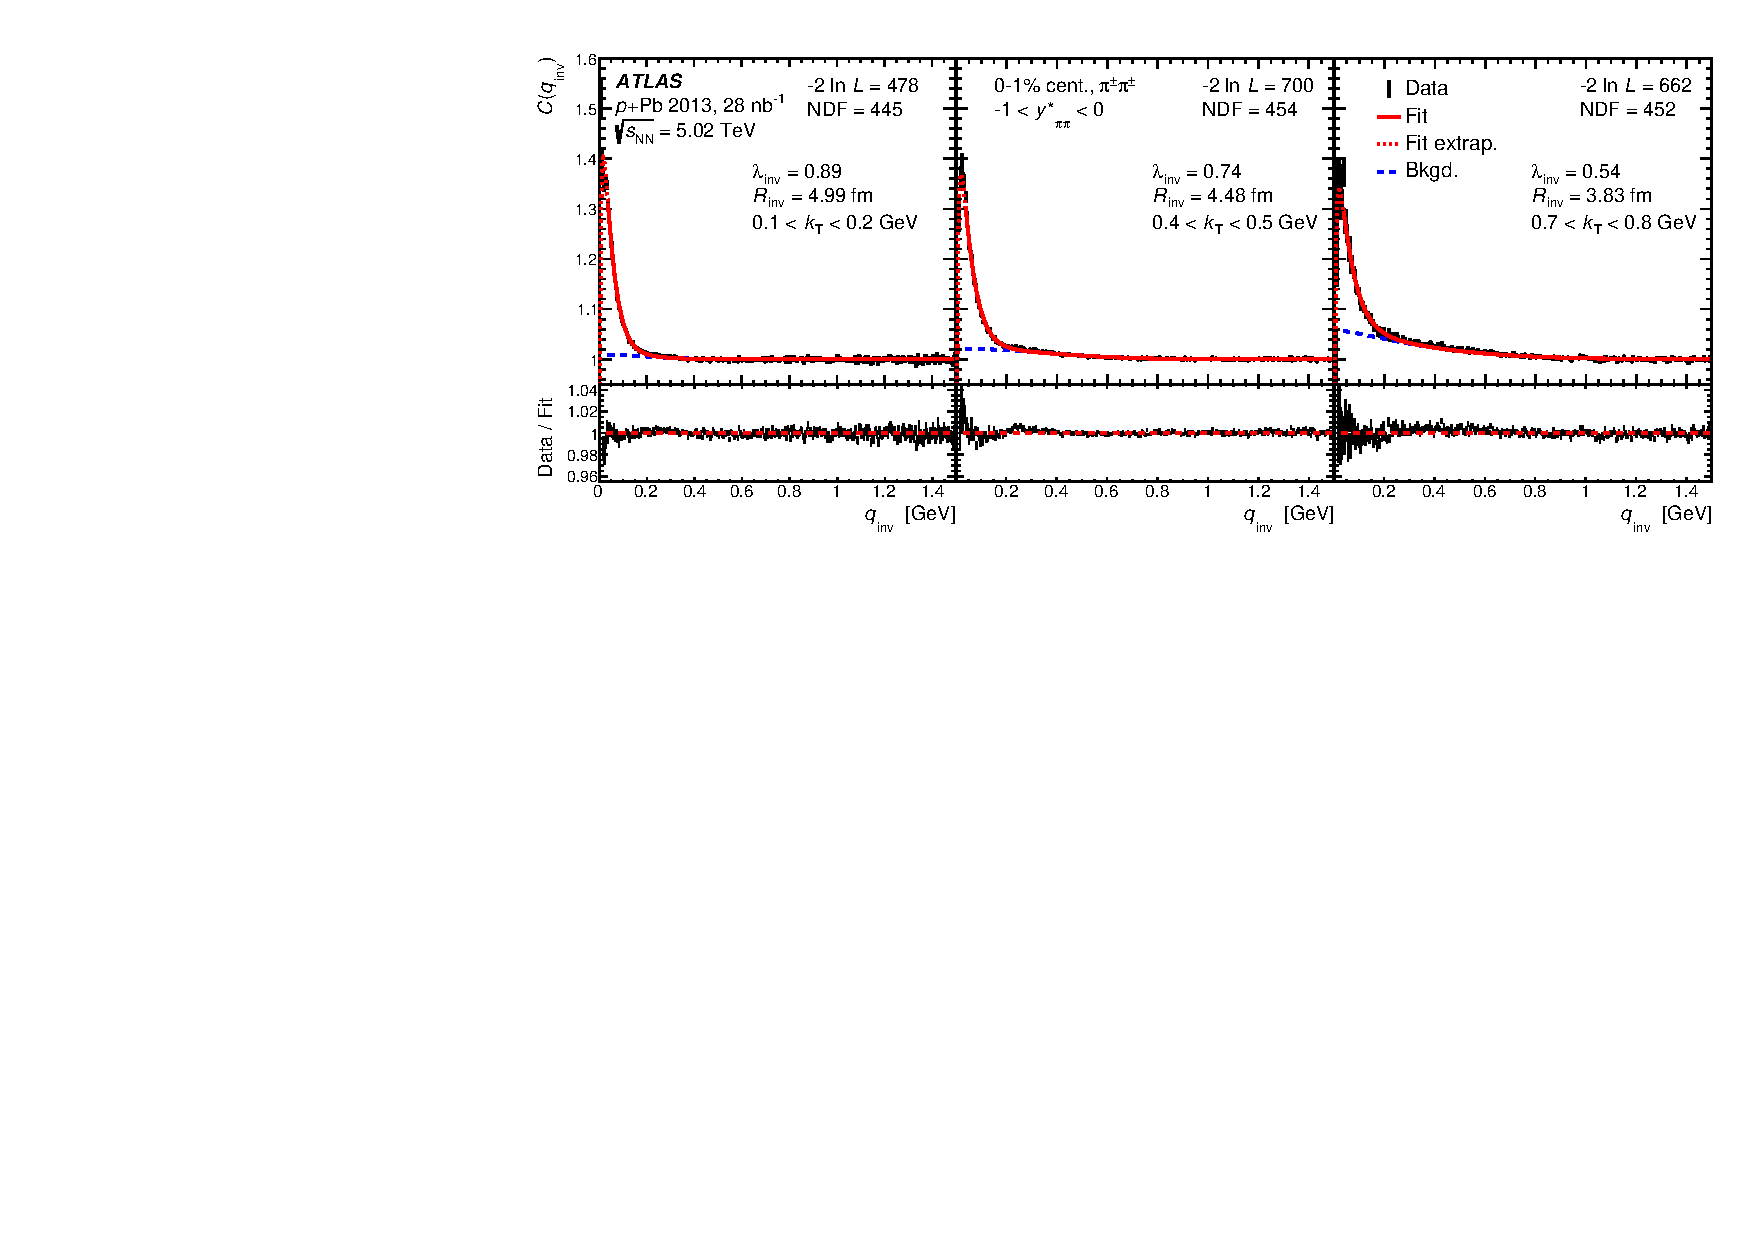
\includegraphics[width=\linewidth]{Cqinv_kt_cent0_e3_kys1.pdf}
\caption{Results of the fit to the one-dimensional correlation function in very central (0--1\%) events in three \kt intervals.
The dashed blue line indicates the description of the contribution from jet fragmentation and the red line shows the full correlation function fit.
The dotted red line indicates the extrapolation of the fit function beyond the interval over which the fit is performed.
}
\label{fig:cqinv_cent0}
\end{figure}

\begin{figure}[t]
\centering
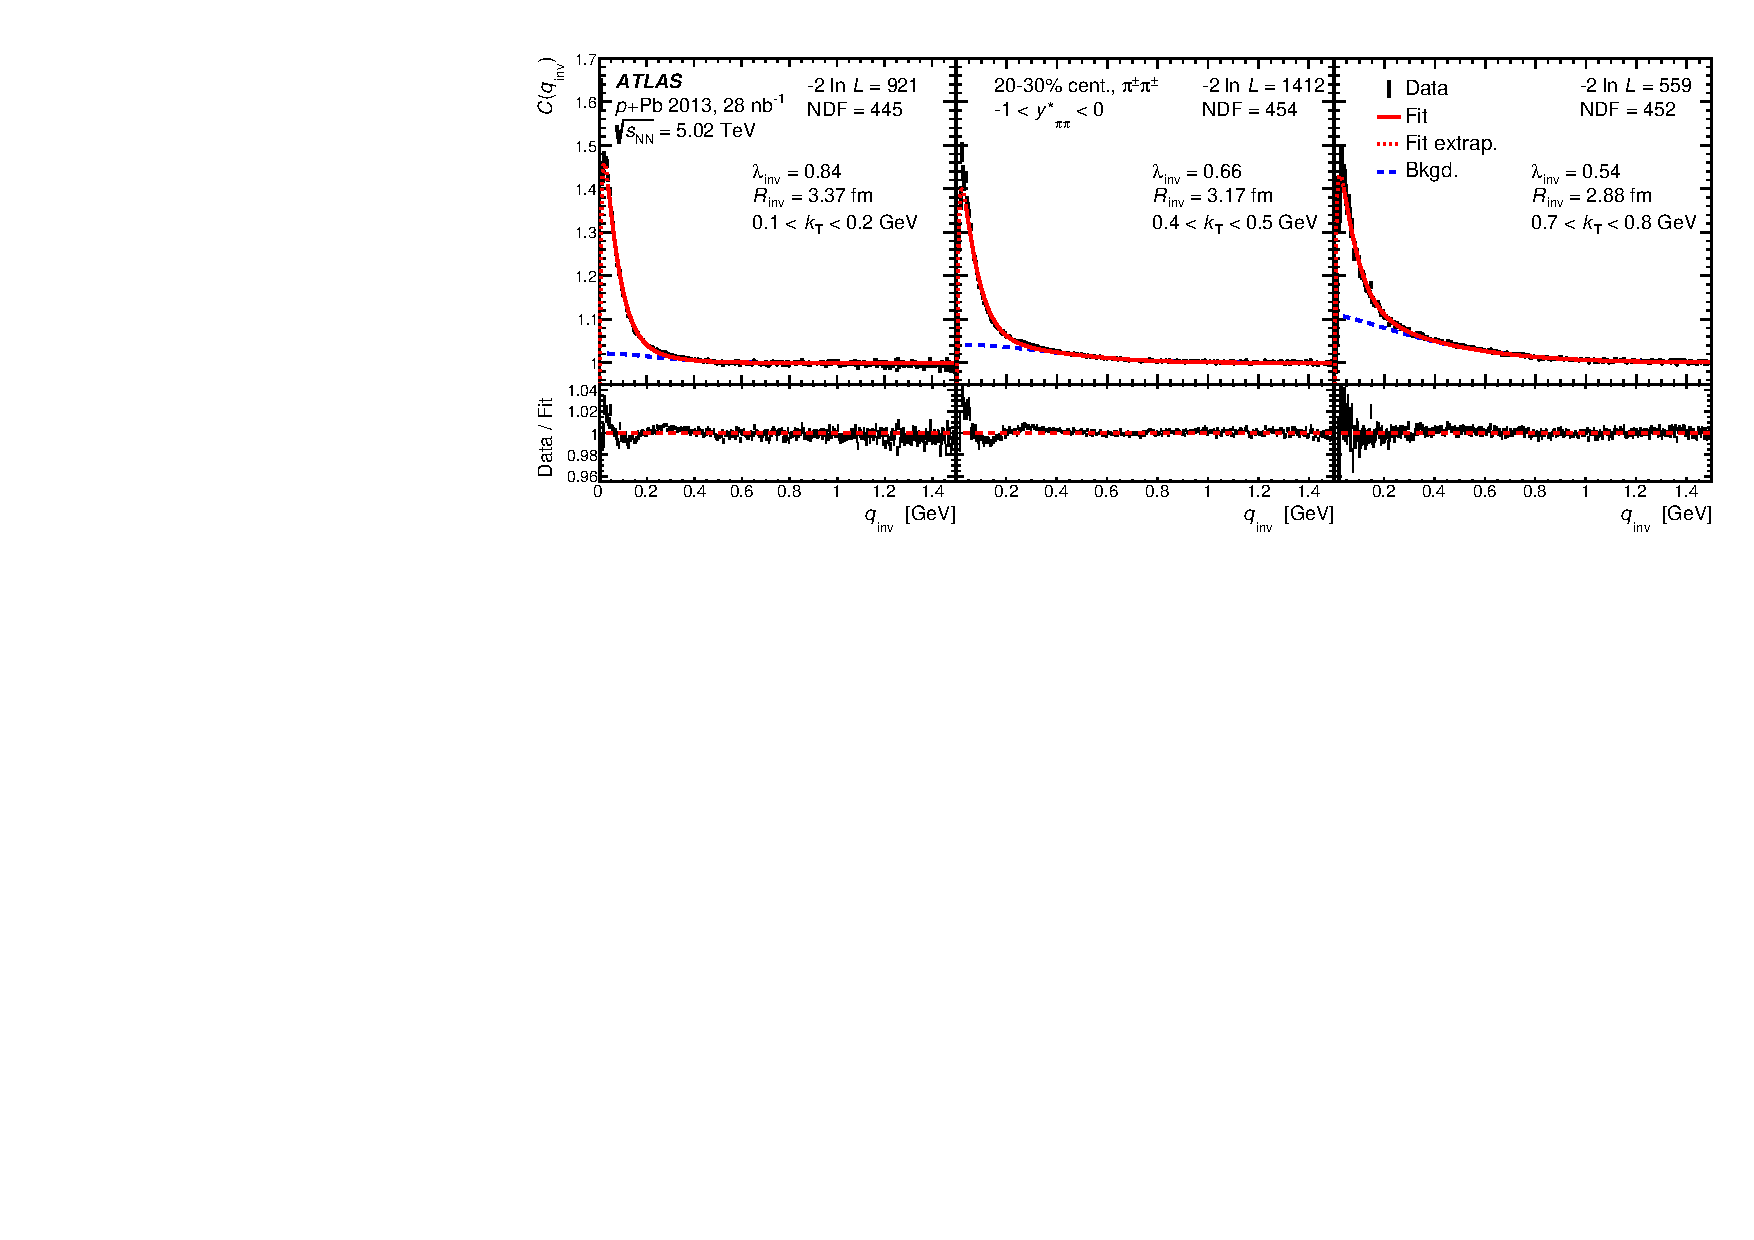
\includegraphics[width=\linewidth]{Cqinv_kt_cent4_e3_kys1.pdf}
\caption{Results of the fit to the one-dimensional correlation function in semi-central (20--30\%) events in three \kt intervals.
The dashed blue line indicates the description of the contribution from jet fragmentation and the red line shows the full correlation function fit.
The dotted red line indicates the extrapolation of the fit function beyond the interval over which the fit is performed.
}
\label{fig:cqinv_cent4}
\end{figure}
\begin{figure}[t]
\centering
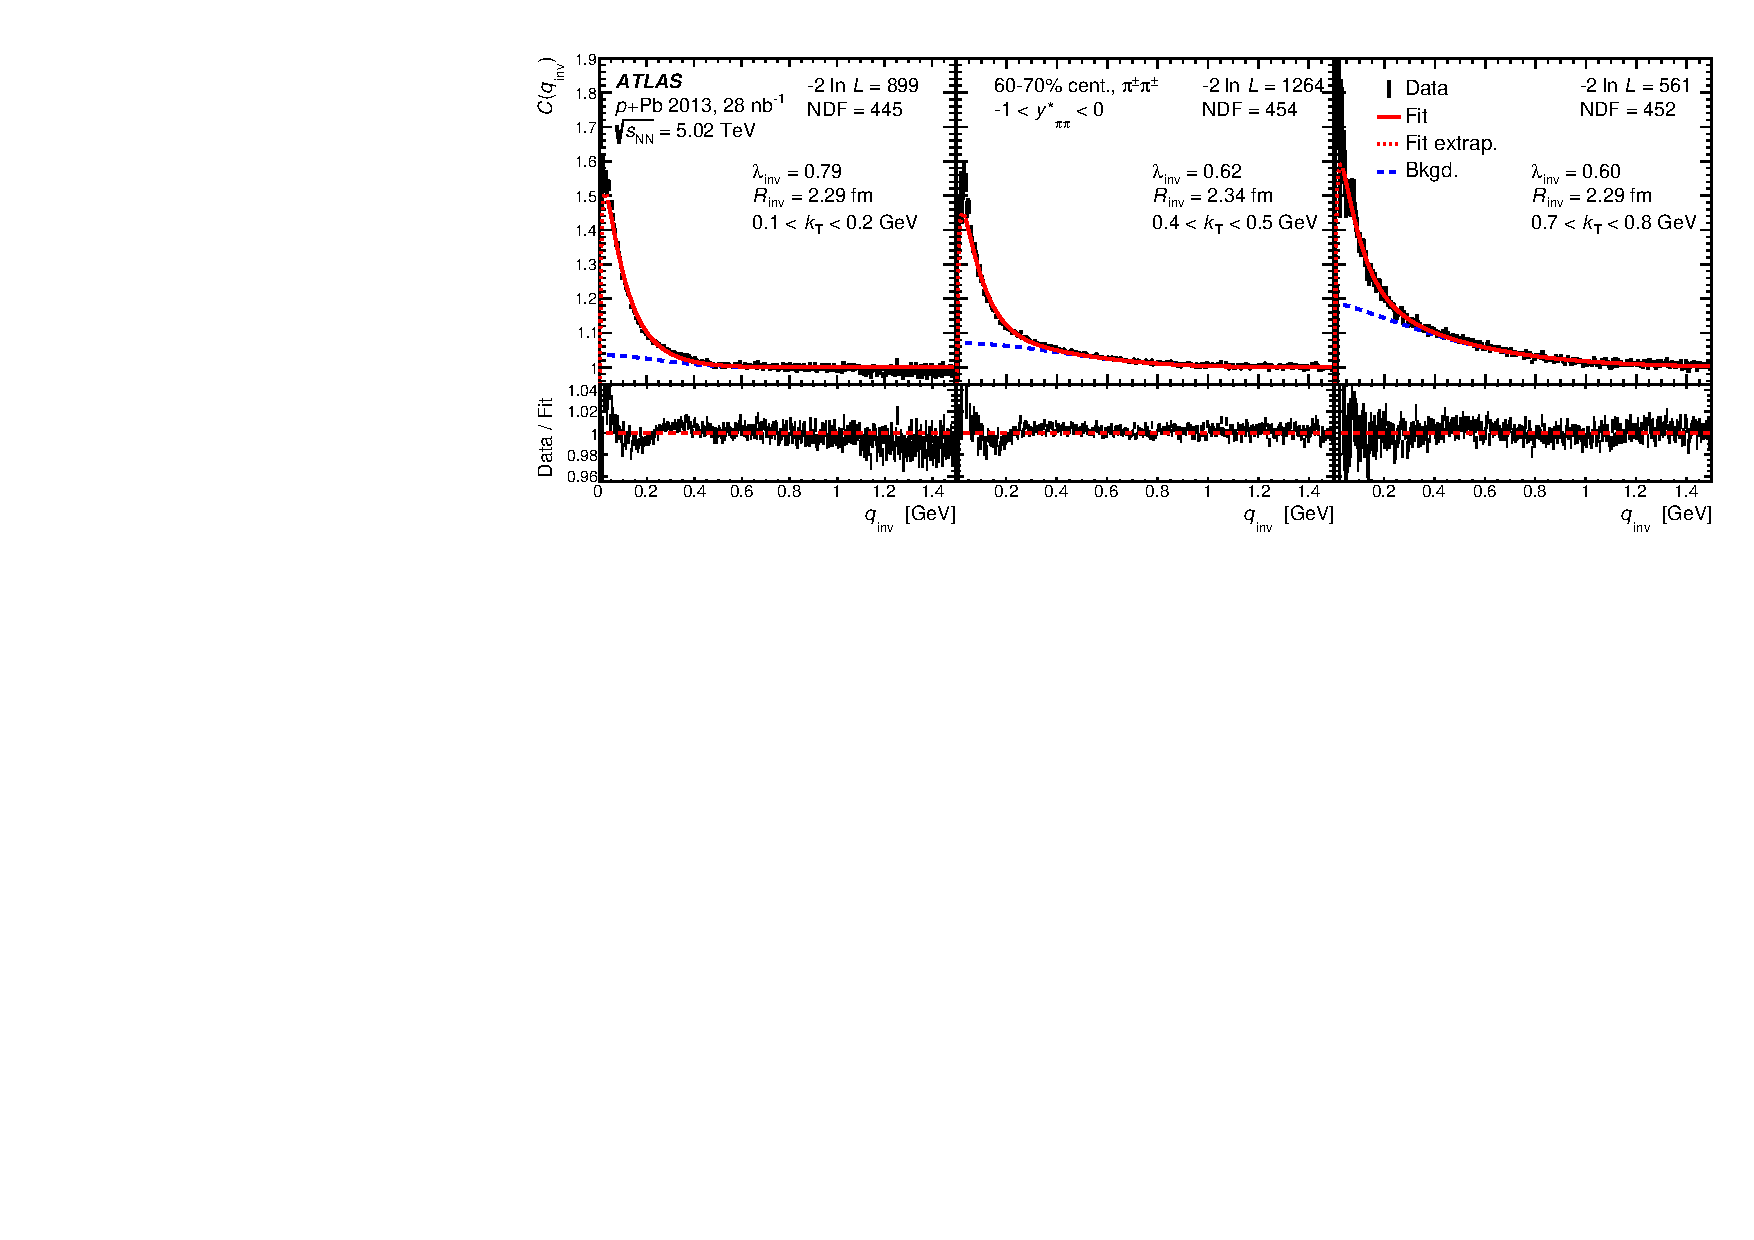
\includegraphics[width=\linewidth]{Cqinv_kt_cent8_e3_kys1.pdf}
\caption{Results of the fit to the one-dimensional correlation function in relatively peripheral (60--70\%) events in three \kt intervals.
The dashed blue line indicates the description of the contribution from jet fragmentation and the red line shows the full correlation function fit.
The dotted red line indicates the extrapolation of the fit function beyond the interval over which the fit is performed.
}
\label{fig:cqinv_cent8}
\end{figure}

An example of a one-dimensional fit to $C(\qinv)$ using the functional form of \cref{eq:correlation_function_full} is included in \cref{fig:hp_example}.
Additional examples of one-dimensional fits for different \kt intervals are shown in \cref{fig:cqinv_cent0,fig:cqinv_cent4,fig:cqinv_cent8} for very central (0--1\%), semi-central (20--30\%), and peripheral (60--70\%) centrality intervals, respectively.
The fits to the same-charge correlation functions generally describe the data well, with only small departures from an exponential description.


\begin{figure}[h]
\centering
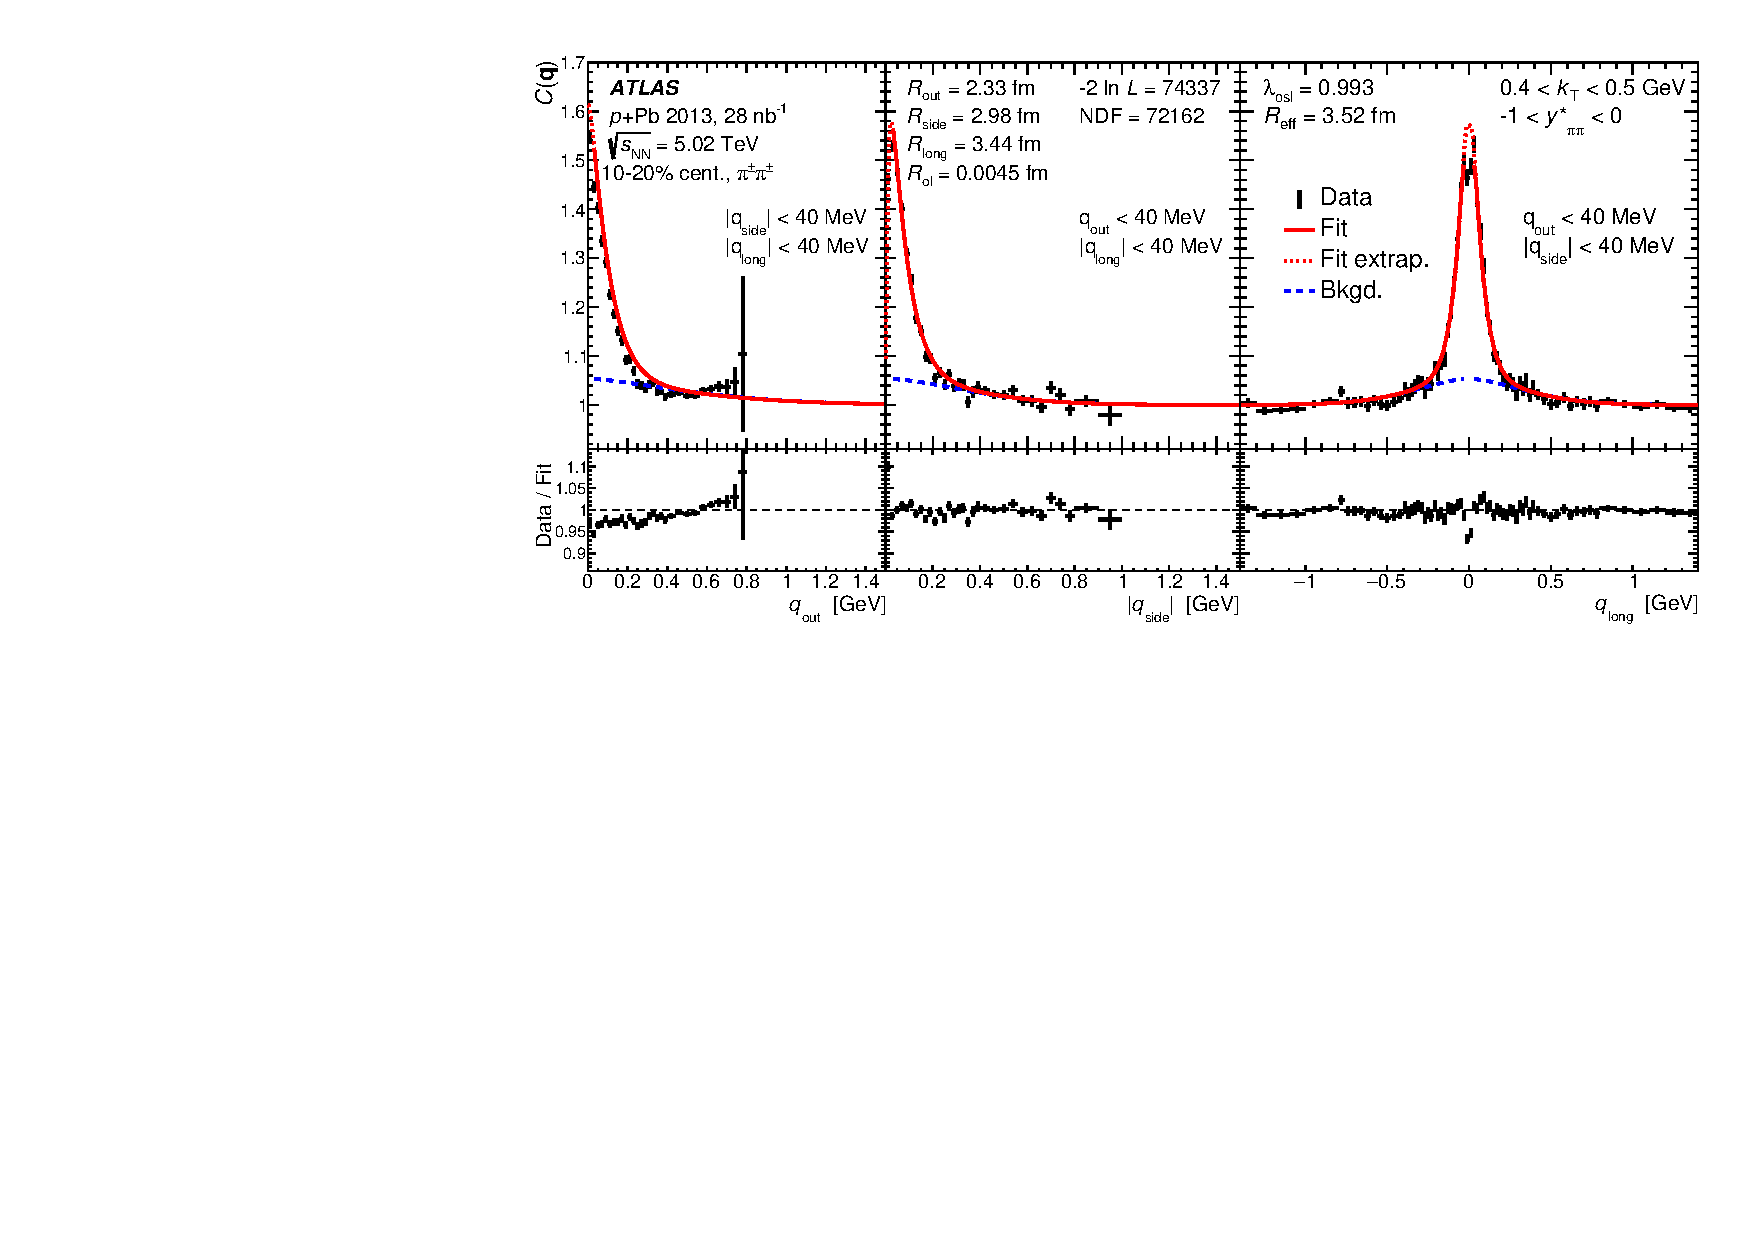
\includegraphics[width=0.97\linewidth]{Cqosl_slices_cent3_e3_kt3_ys1.pdf}
\caption{Results of the 3D fit to the correlation function in the $0.4 < \kt < 0.5$~\GeV, $-1 < \kys < 0$ kinematic intervals and for the 10--20\% centrality interval.
The left, middle, and right panels show the distributions versus \qout, \qside, and \qlong, respectively, with limits on the other two components of $\mathbf{q}$ such that $|q_i| < 40~\MeV$.
The dashed blue line indicates the description of the contribution from hard processes and the red line shows the full correlation function fit.
The dotted red line indicates the extrapolation of the fit function beyond the interval over which the fit is performed.
}
\label{fig:cqosl_slices}
\end{figure}


Slices of a three-dimensional fit of $C(\mathbf{q})$ to the three-dimensional variant of \cref{eq:correlation_function_full} are shown in \cref{fig:cqosl_slices}.
The apparently imperfect fit along the \qout axis is characteristic of $\qside \approx \qlong \approx 0$, and away from this slice the  fit agrees better with the data (the test statistic per degree of freedom is 1.03 for the fit shown). 



\FloatBarrier
\section{HBT radii}
\subsection{Lorentz invariant results}
\label{subsec:invariant_results}

\begin{figure}[t]
\centering
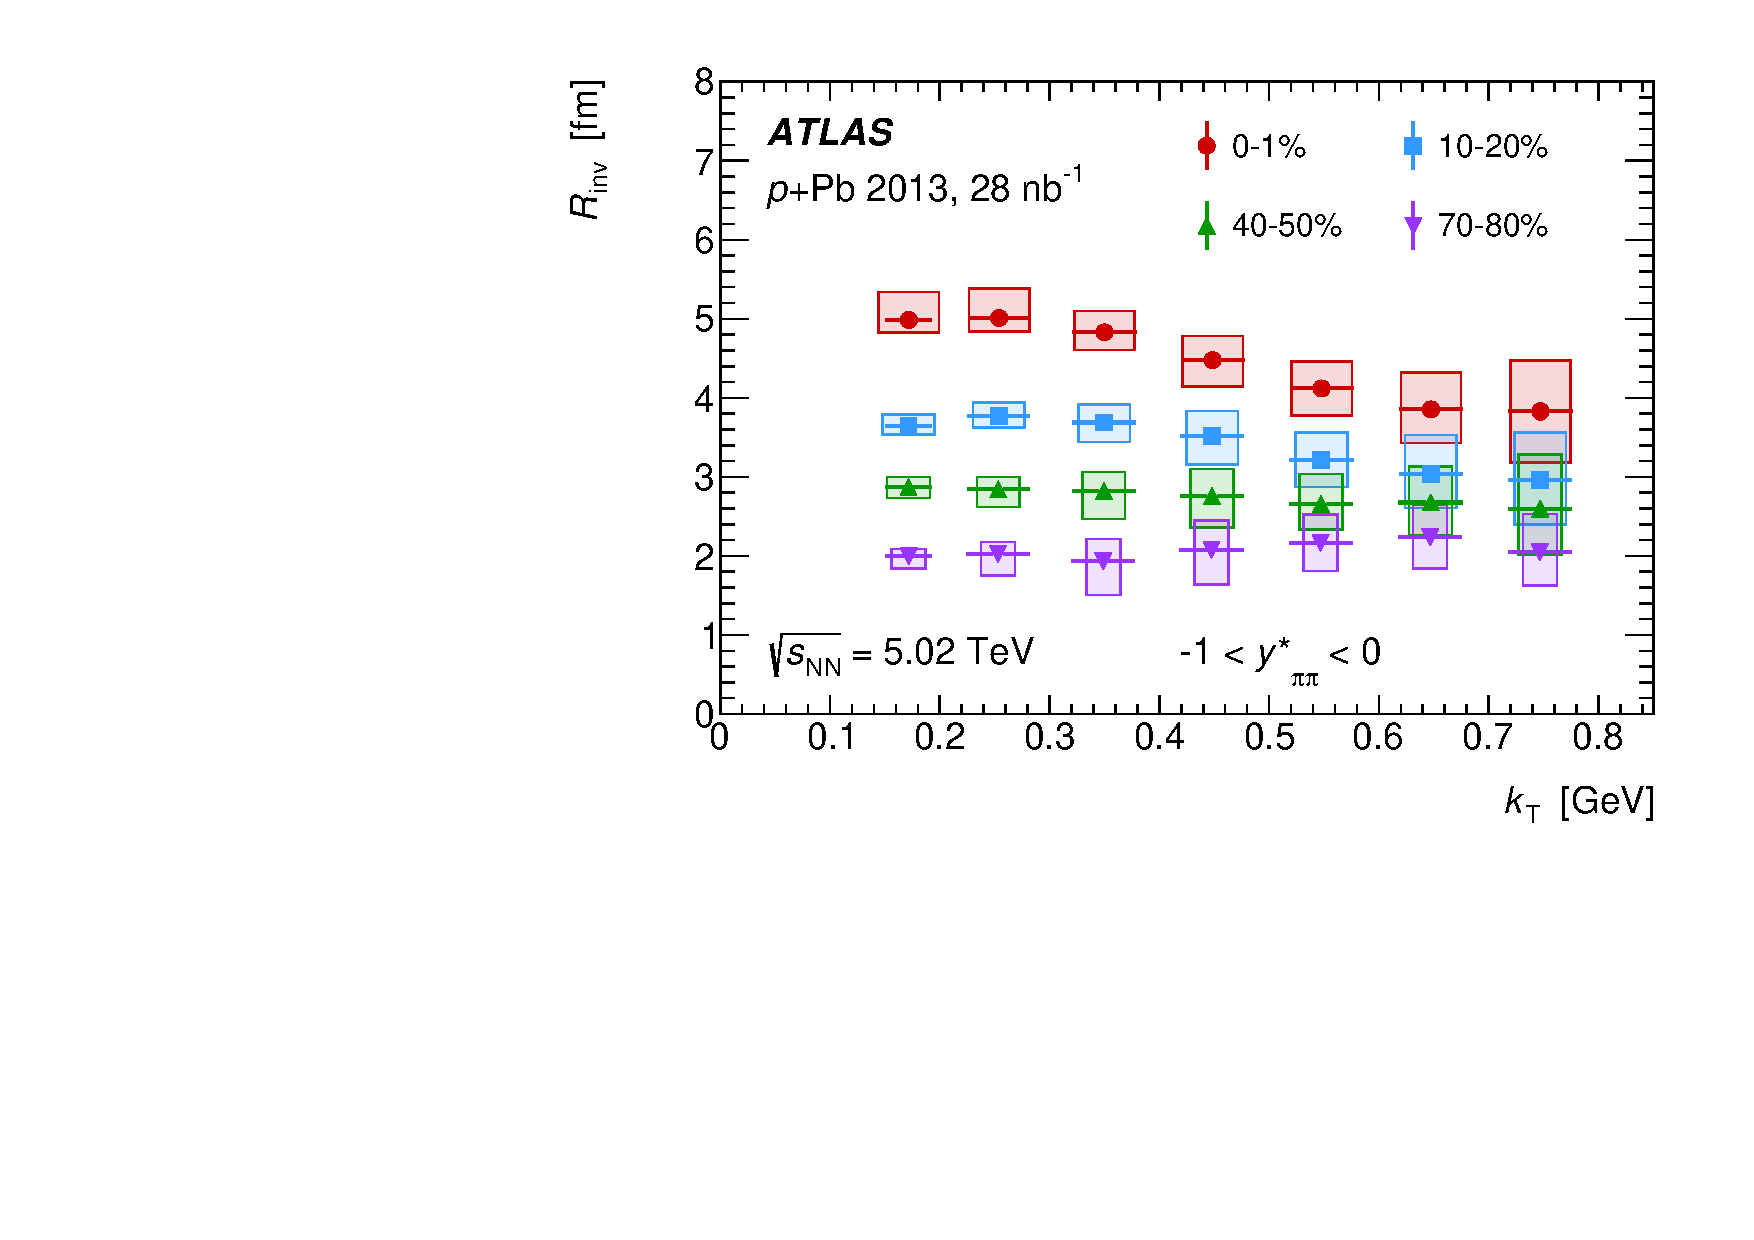
\includegraphics[width=0.49\linewidth]{canqinv_R_vs_kt.pdf}
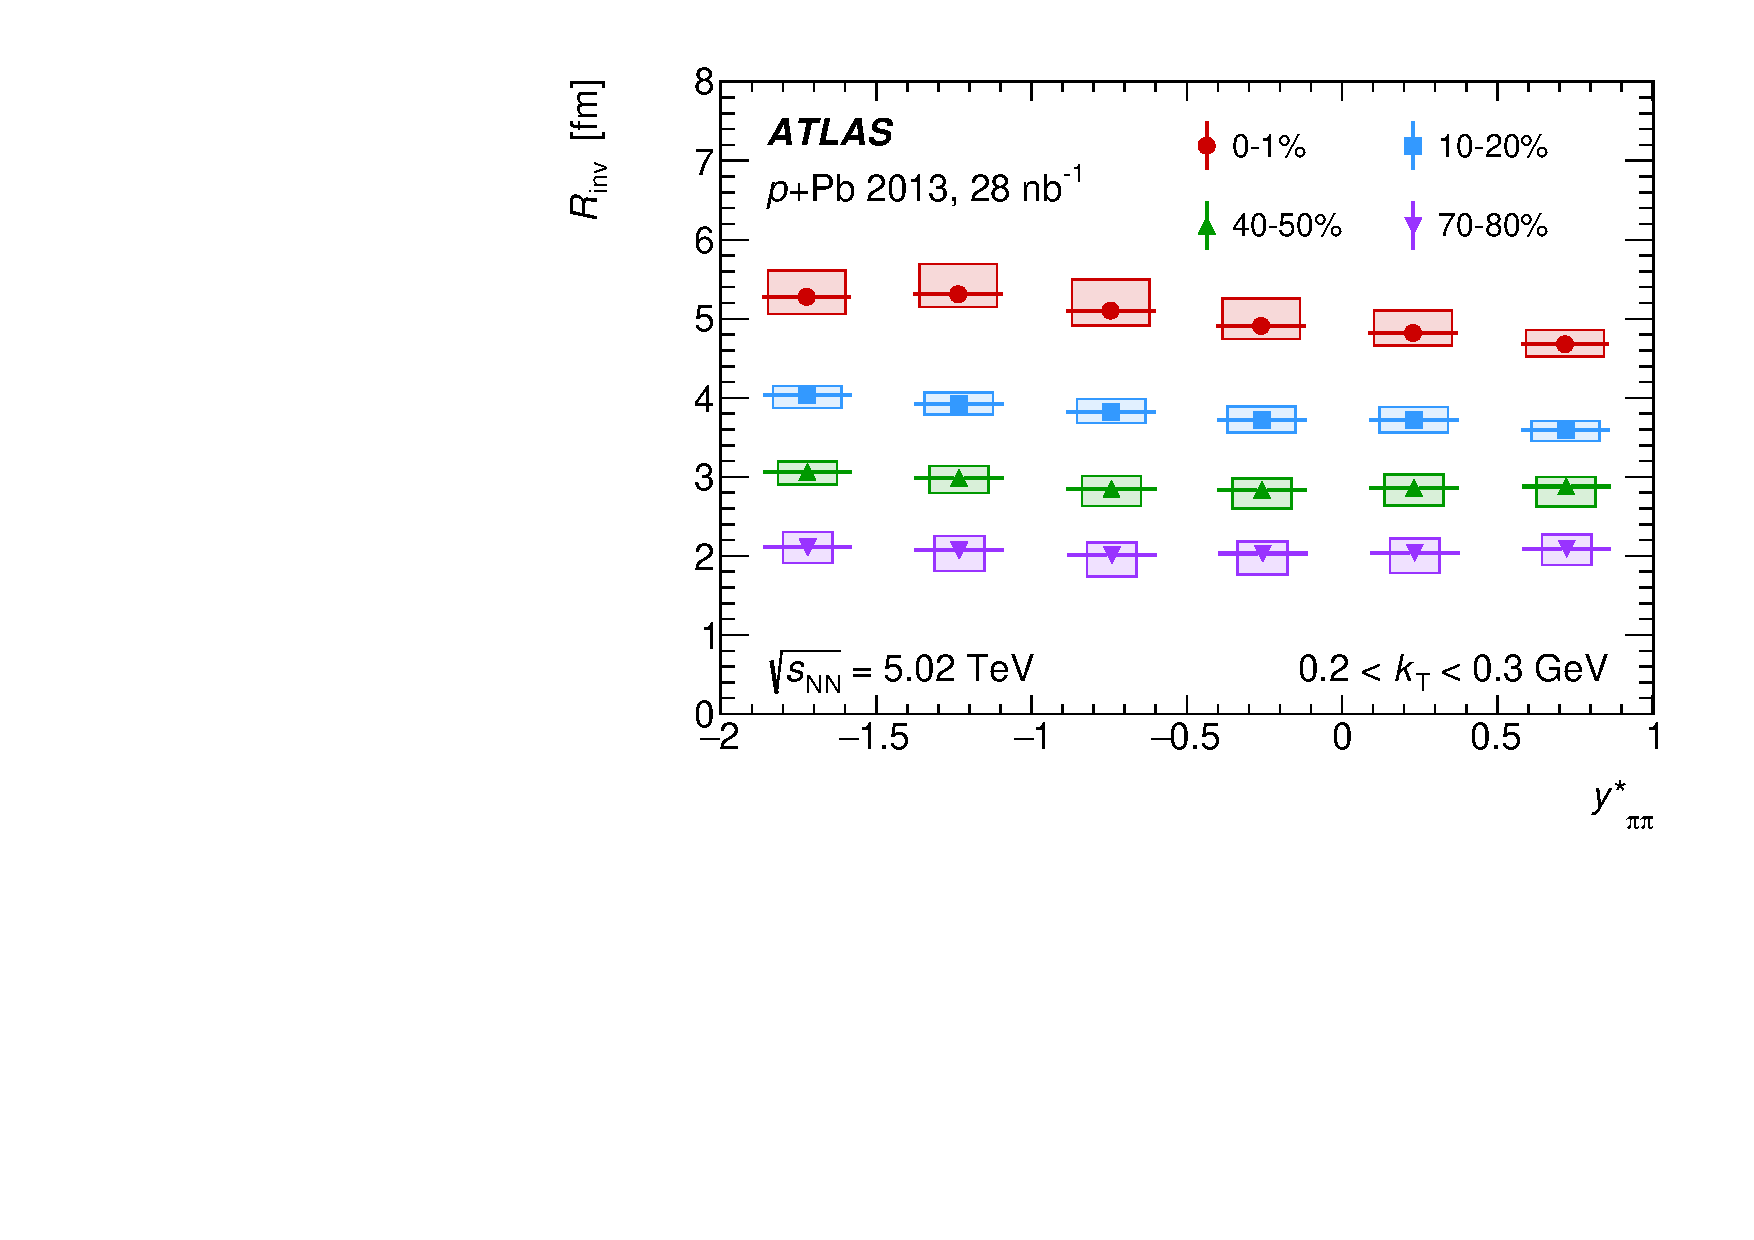
\includegraphics[width=0.49\linewidth]{canqinv_R_vs_kys.pdf}
\caption{The exponential invariant radii, \Rinv, obtained from one-dimensional fits to
the \qinv\ correlation functions shown as a function of pair transverse momentum, \kt, (left) and rapidity, \kys (right). Four non-adjacent centrality intervals are shown. The vertical size of each box represents the quadrature sum of the systematic uncertainties described in \cref{sec:systematics}, and statistical uncertainties are shown with vertical lines. The horizontal positions of the points are the average \kt or \kys in each interval, and the horizontal lines indicate the standard deviation of \kt or \kys. The widths of the boxes differ among centrality intervals only for visual clarity.}
\label{fig:results_Rinv_kt}
\end{figure}
\begin{figure}[t]
\centering
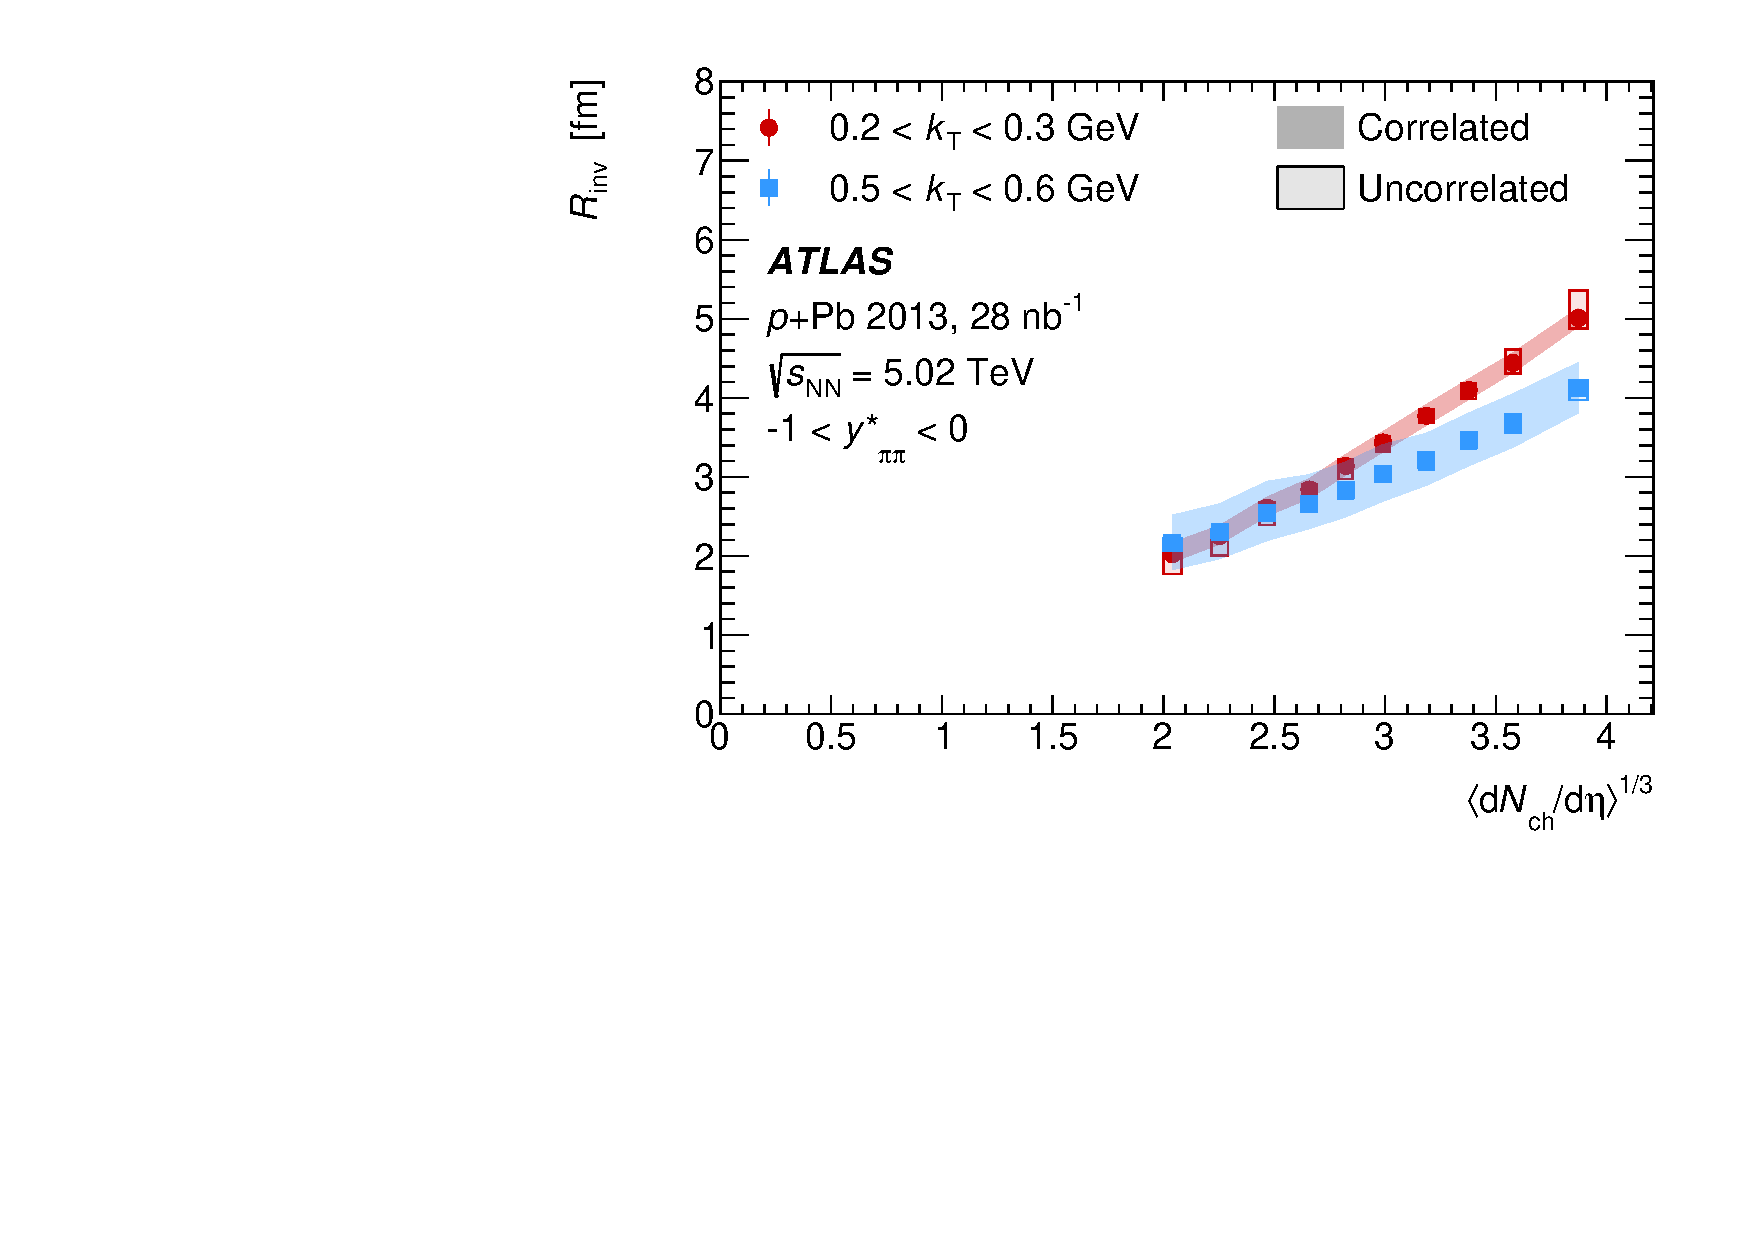
\includegraphics[width=0.49\linewidth]{canqinv_R_vs_avg_mult.pdf}
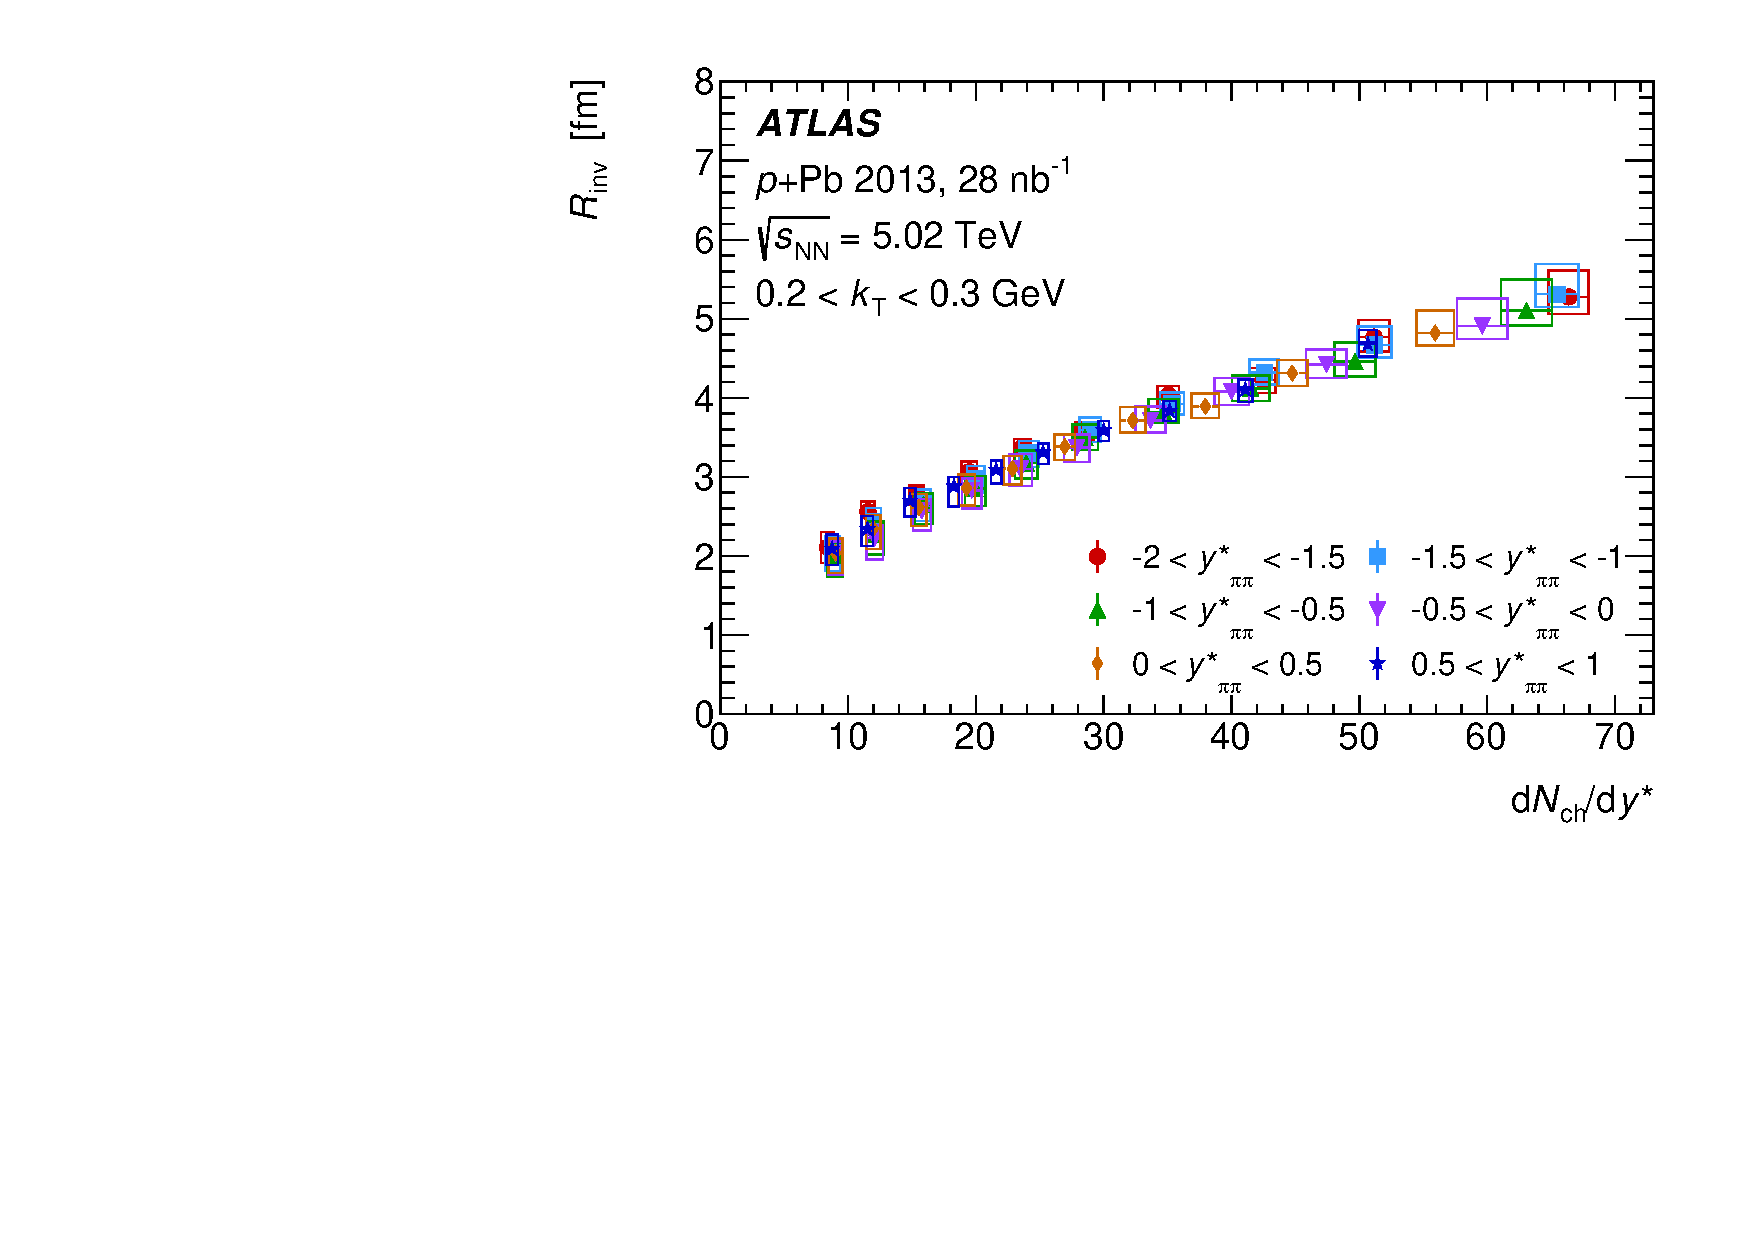
\includegraphics[width=0.49\linewidth]{canqinv_R_kt1_vs_mult.pdf}
\caption{Exponential fit results for $\Rinv$ as a function of the cube root of average charged-particle multiplicity $\avgdNdeta^{1/3}$ (left), where the average is taken over $|\eta| < 1.5$, and as a function of the local density, \dNdy, over several centrality and rapidity intervals (right). In the left plot the systematic uncertainties from pion identification and from the generator and collision system components of the background amplitude are treated as correlated and shown as error bands, and the systematic uncertainties from charge asymmetry, \Reff, the rapidity variation of the jet fragmentation description, and two-particle reconstruction are treated as uncorrelated and indicated by the height of the boxes. The horizontal error bars indicate the systematic uncertainty from \avgdNdeta or \dNdy.}
\label{fig:results_Rinv_dndeta}
\end{figure}

The results from fits of $C(\qinv)$ to \cref{eq:correlation_function_full} for the invariant radius, \Rinv, are shown in \cref{fig:results_Rinv_kt} in four selected centrality intervals.
Only an intermediate rapidity interval $-1 < \kys < 0$ is shown for these and similar results as a function of \kt, as the qualitative behavior is consistent in forward and backward rapidities.
The clear decrease in size with increasing \kt that is observed in central events is not observed in peripheral events.
This is consistent with the interpretation that central events undergo transverse expansion, since in hydrodynamic models higher-\pt particles are more likely to freeze out earlier in the event.
Another way of understanding this trend as evidence for transverse expansion is that there is a smaller homogeneity region for particles with higher \pt \cite{Kolb:2003dz}.
At low \kt, ultra-central (0--1\%) events have an invariant radius significantly greater than peripheral (70--80\%) events by a factor of about 2.6.
This difference becomes less prominent at high \kt.
In central events \Rinv is larger on the lead-going side than on the proton-going side, while in peripheral events the rapidity dependence of the radius becomes constant.

Invariant radii are shown for several centralities in \cref{fig:results_Rinv_dndeta} (left) as a function of the cube root of average \dNdeta. 
For both \kt intervals shown, the scaling of \Rinv with $\avgdNdeta^{1/3}$ is close to linear but with a slightly increasing slope at higher multiplicities.
The invariant radius, \Rinv, has a steeper trend versus multiplicity at lower \kt.
\cref{fig:results_Rinv_dndeta} (right) shows \Rinv in several centrality and rapidity intervals as a function of the local particle density, \dNdy, which is evaluated by taking the average over the same interval used for the pair's rapidity.
The extracted radius and the local particle density are seen to be tightly correlated, such that the radius can be predicted, within uncertainties, by the local density alone.

\begin{figure}[t]
\centering
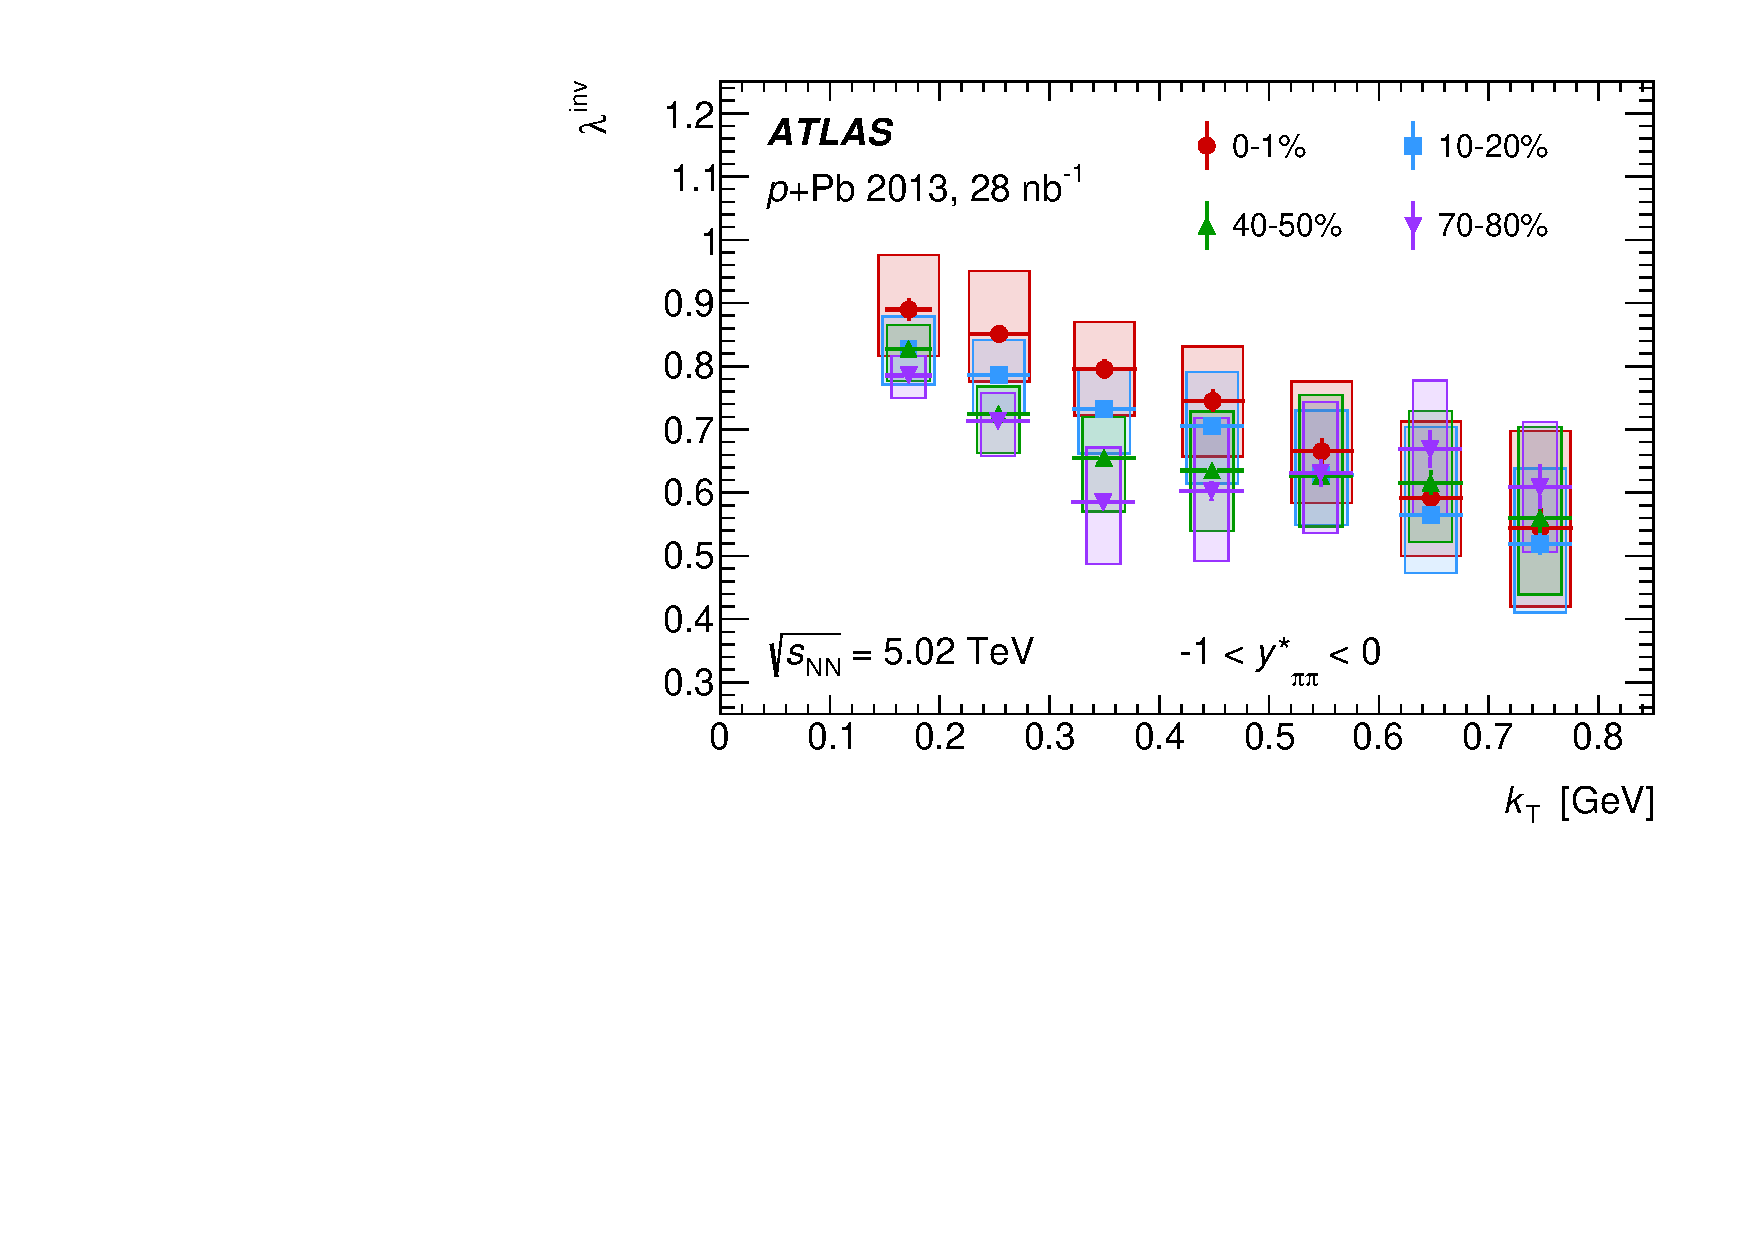
\includegraphics[width=0.49\linewidth]{canqinv_x_vs_kt.pdf}
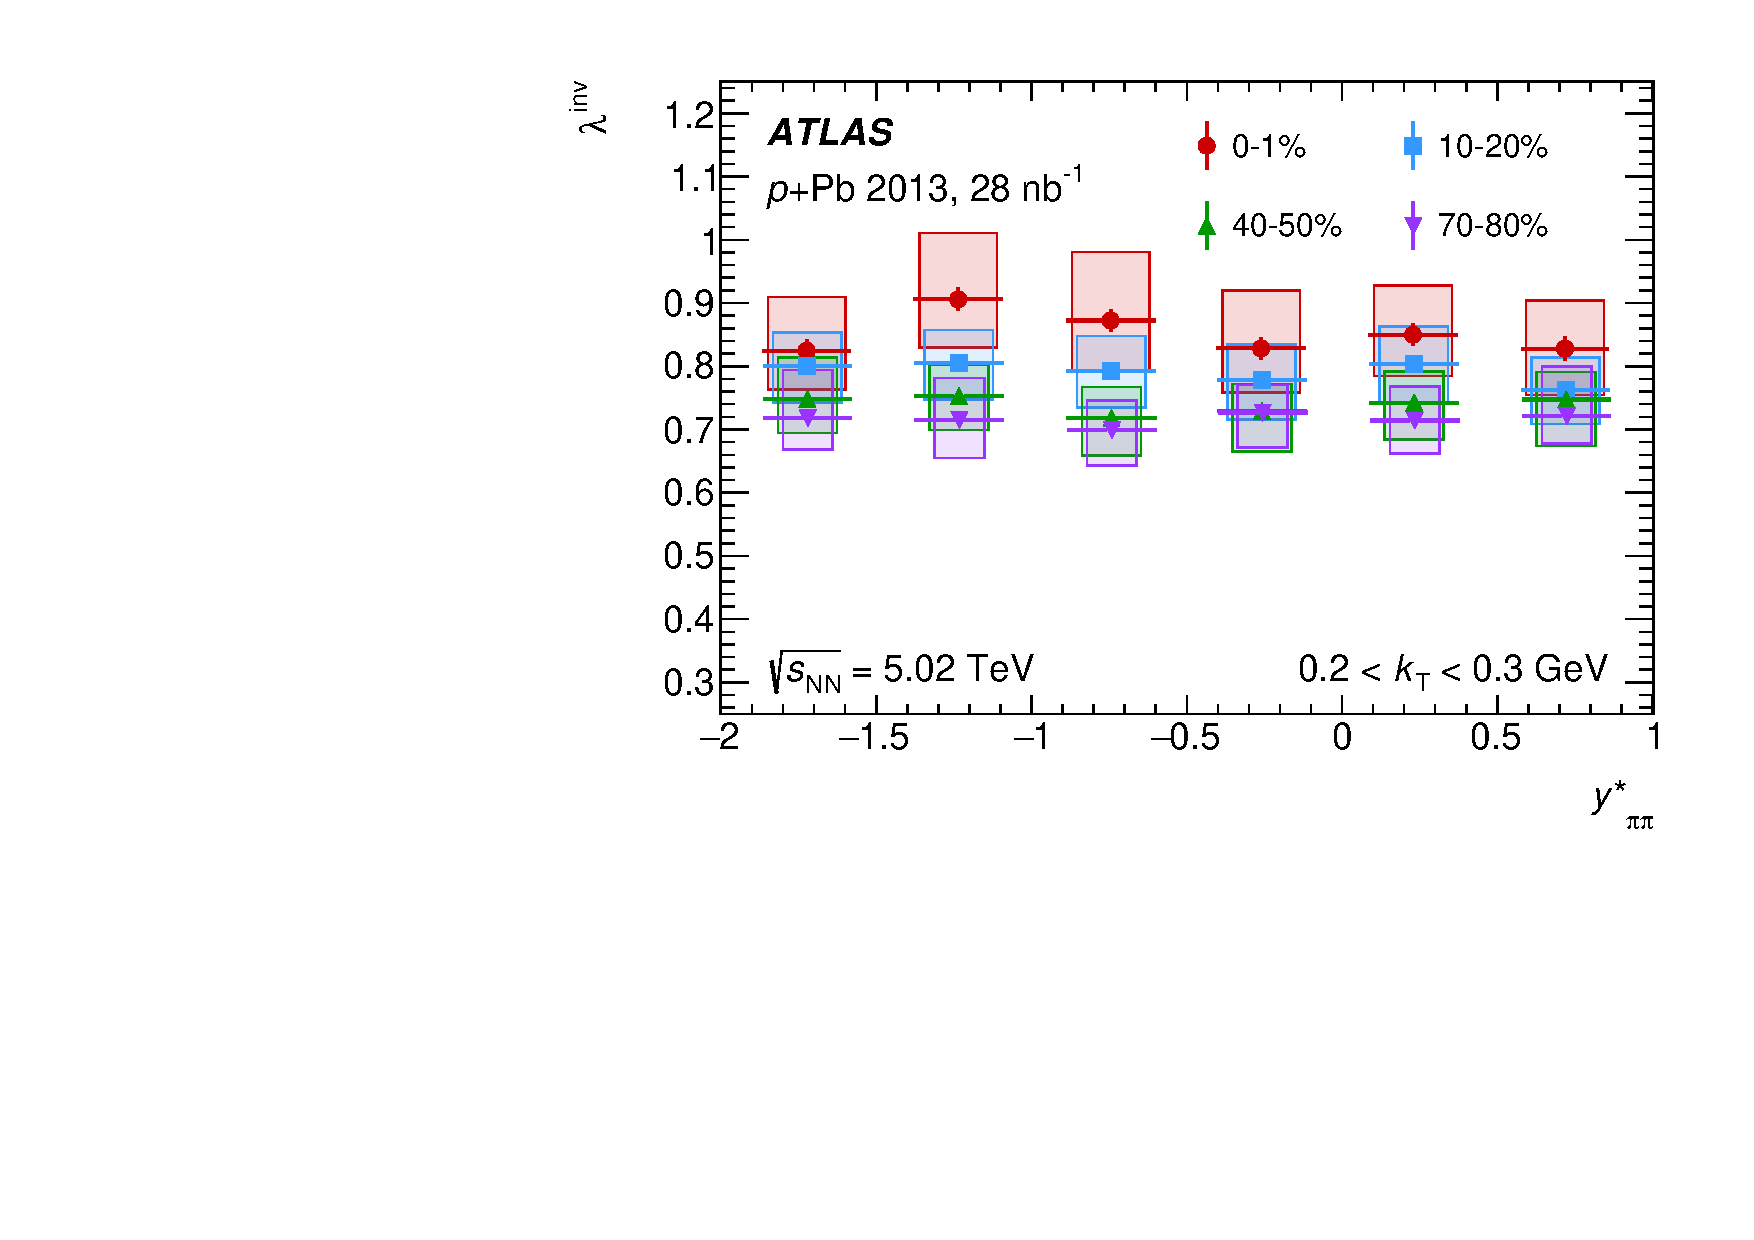
\includegraphics[width=0.49\linewidth]{canqinv_x_vs_kys.pdf}
\caption{The Bose-Einstein amplitude, \linv, obtained from one-dimensional fits to the \qinv\ correlation functions shown as a function of pair transverse momentum, \kt, (left) and rapidity, \kys (right). Four non-adjacent centrality intervals are shown. The vertical size of each box represents the quadrature sum of the systematic uncertainties described in \cref{sec:systematics}, and statistical uncertainties are shown with vertical lines. The horizontal positions of the points are the average \kt or \kys in each interval, and the horizontal lines indicate the standard deviation of \kt or \kys. The widths of the boxes differ among centrality intervals only for visual clarity.}
\label{fig:results_qinv_x}
\end{figure}

The Bose-Einstein amplitude of the invariant fits, \linv, is shown in \cref{fig:results_qinv_x} as a function of \kt and \kys.
At low \kt, \linv has values near unity, and it decreases with rising \kt.
In the lower \kt intervals a systematic difference is observed between centrality intervals, with \linv having larger values in central events.
In contrast, at larger \kt the amplitudes are indistinguishable between different centralities.
The amplitude exhibits no significant variation over rapidity.

\FloatBarrier
\subsection{Three-dimensional radii}
\label{subsec:3d_results}

\begin{figure}[ht]
\centering
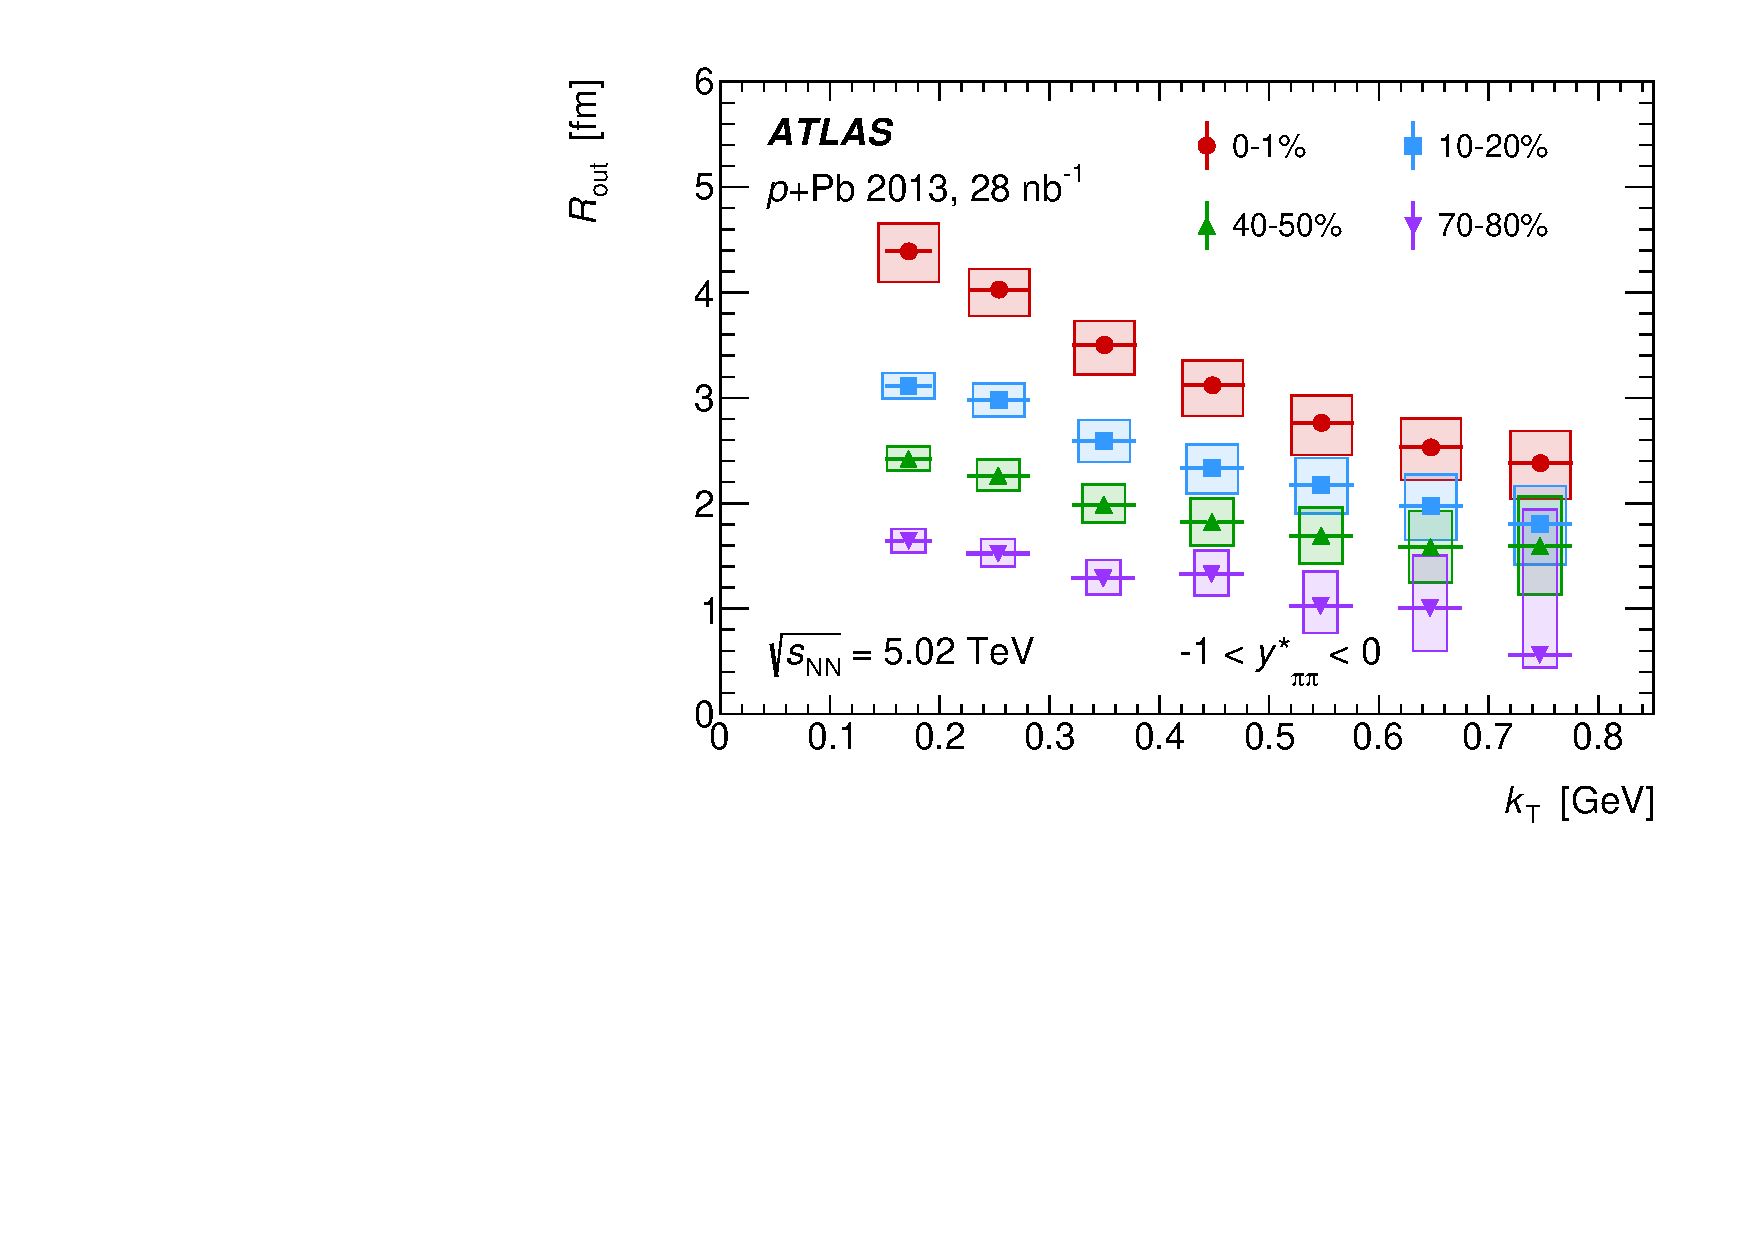
\includegraphics[width=.49\linewidth]{canqosl_Rout_vs_kt.pdf}
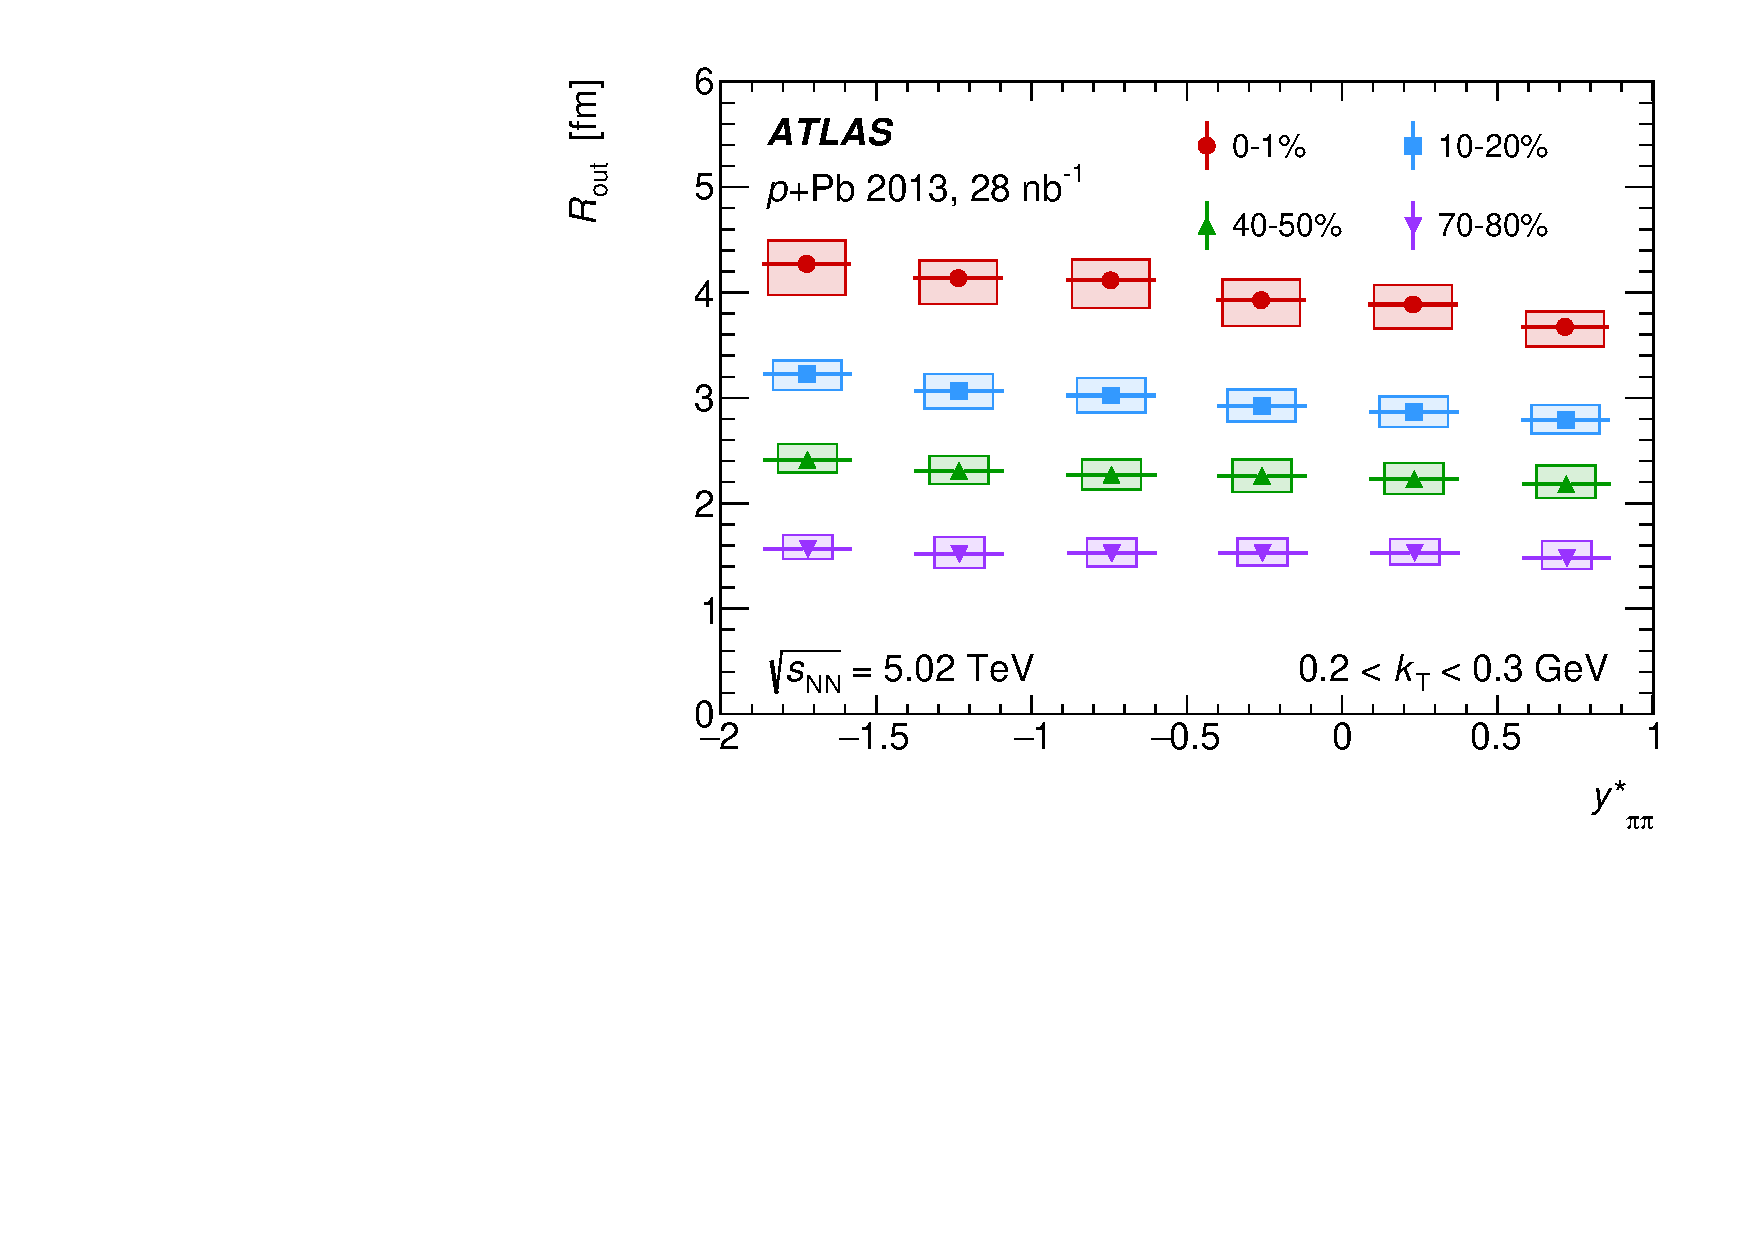
\includegraphics[width=.49\linewidth]{canqosl_Rout_vs_kys.pdf}
\caption{Exponential fit results for the 3D source radius, \Rout, as a function of pair transverse momentum, \kt, (left) and rapidity, \kys (right). Four non-adjacent centrality intervals are shown. The vertical size of each box represents the quadrature sum of the systematic uncertainties described in \cref{sec:systematics}, and statistical uncertainties are shown with vertical lines. The horizontal positions of the points are the average \kt or \kys in each interval, and the horizontal lines indicate the standard deviation of \kt or \kys. The widths of the boxes differ among centrality intervals only for visual clarity.}
\label{fig:results_Rout}
\end{figure}

\begin{figure}[ht]
\centering
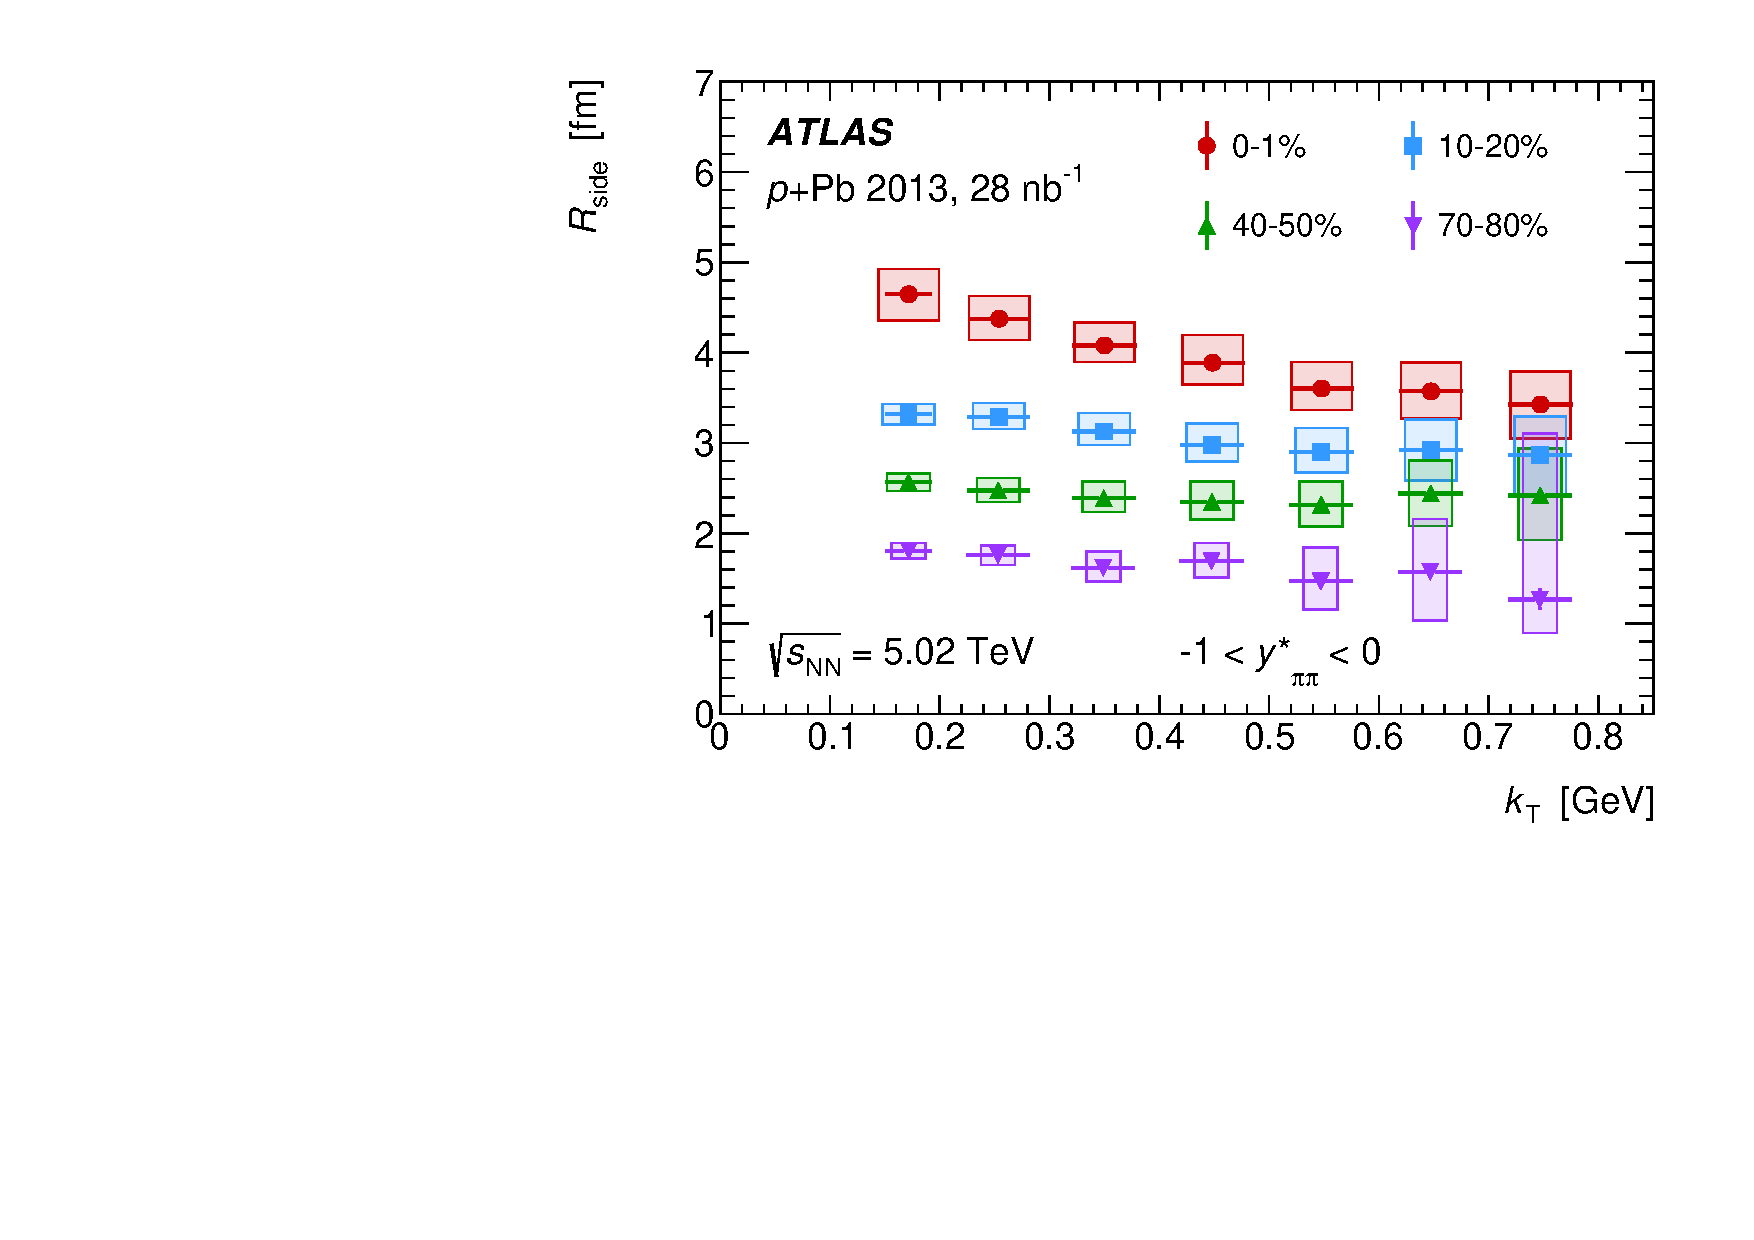
\includegraphics[width=.49\linewidth]{canqosl_Rside_vs_kt.pdf}
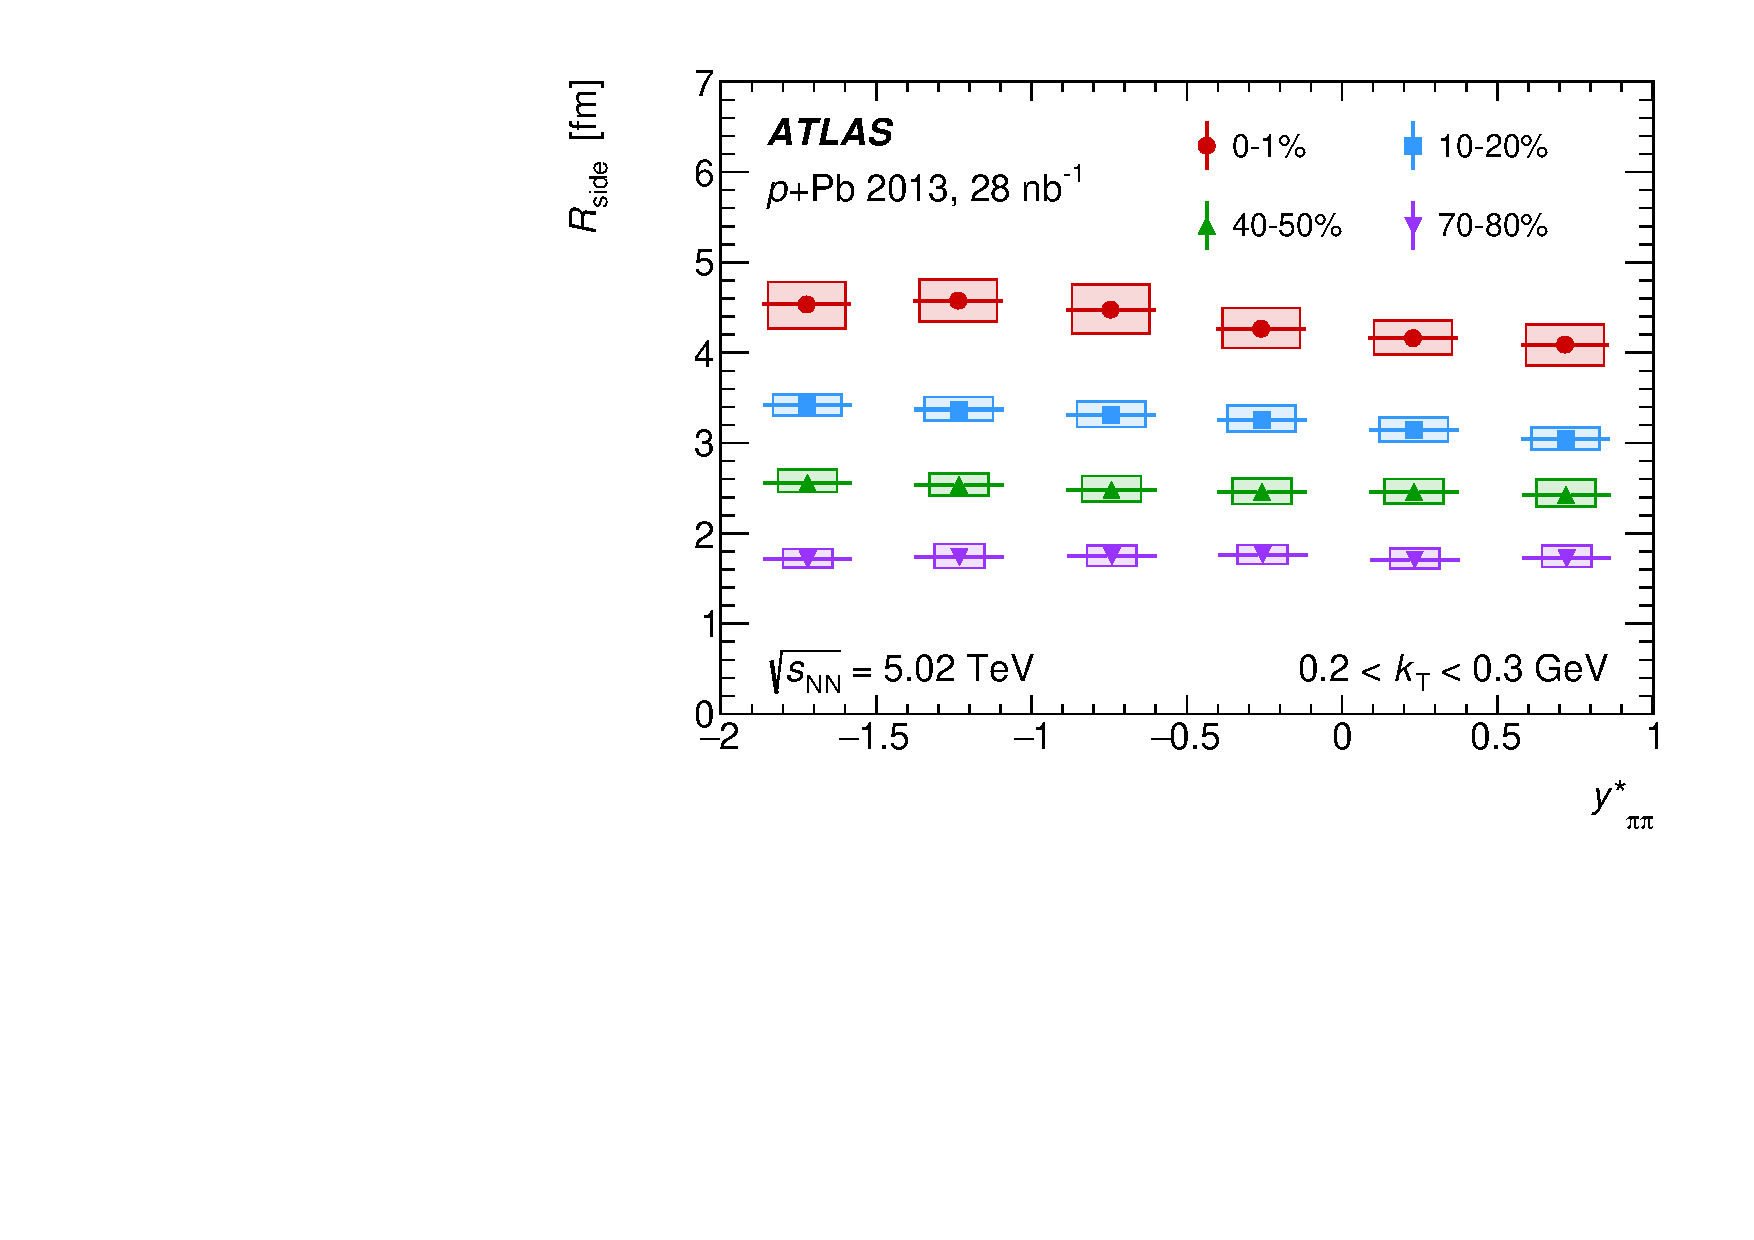
\includegraphics[width=.49\linewidth]{canqosl_Rside_vs_kys.pdf}
\caption{Exponential fit results for the 3D source radius, \Rside, as a function of pair transverse momentum, \kt, (left) and rapidity, \kys (right). Four non-adjacent centrality intervals are shown. The vertical size of each box represents the quadrature sum of the systematic uncertainties described in \cref{sec:systematics}, and statistical uncertainties are shown with vertical lines. The horizontal positions of the points are the average \kt or \kys in each interval, and the horizontal lines indicate the standard deviation of \kt or \kys. The widths of the boxes differ among centrality intervals only for visual clarity.}
\label{fig:results_Rside}
\end{figure}


The three-dimensional radii \Rout, \Rside, and \Rlong are shown as a function of \kt and \kys in four selected centrality intervals in \cref{fig:results_Rout,fig:results_Rside,fig:results_Rlong}.
In central collisions, the 3D radii exhibit an even steeper decrease with increasing \kt relative to that observed for the invariant radii in \cref{fig:results_Rinv_kt}.
A similar, but weaker trend is present in peripheral events.
Central collisions exhibit larger radii on the backward (Pb-going) side of the event, while peripheral events show no distinguishable variation of the radii with rapidity.

\begin{figure}[ht]
\centering
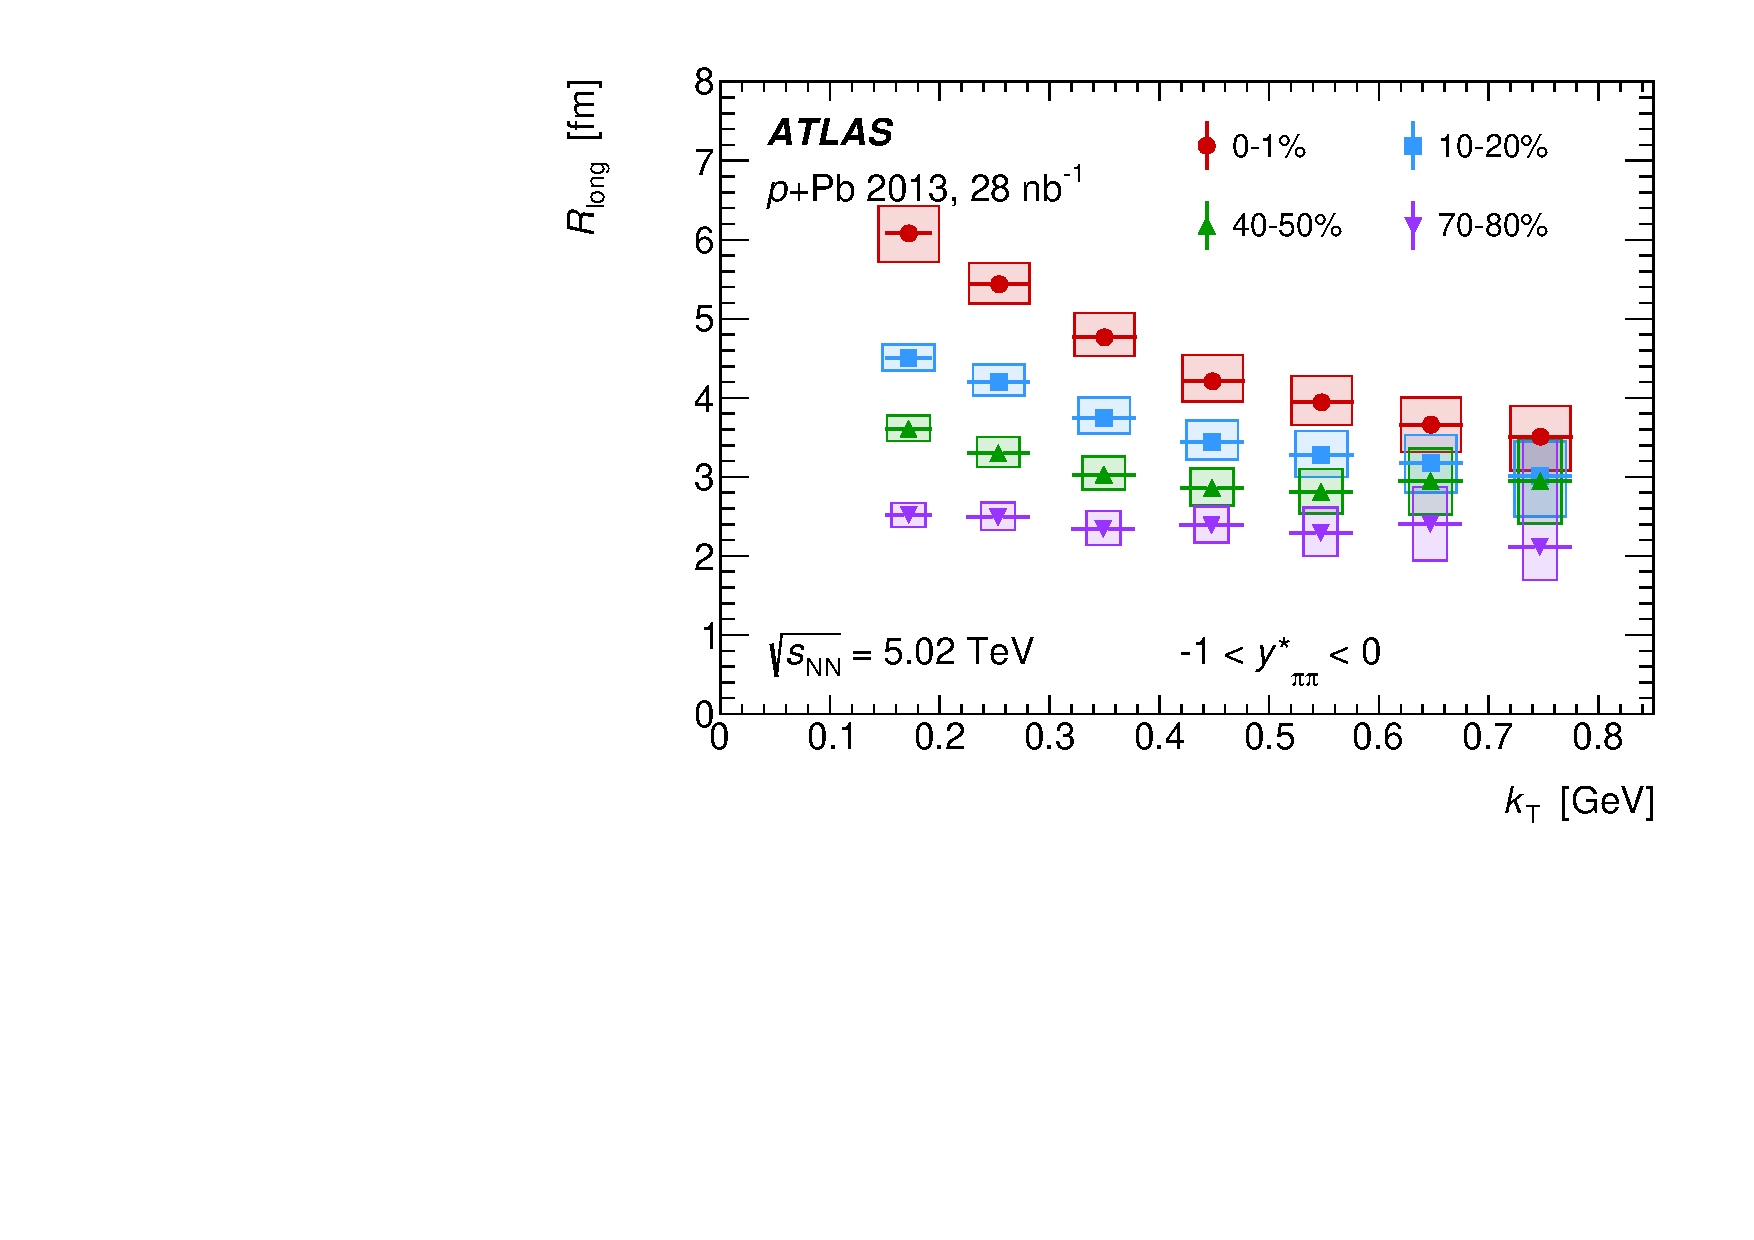
\includegraphics[width=.49\linewidth]{canqosl_Rlong_vs_kt.pdf}
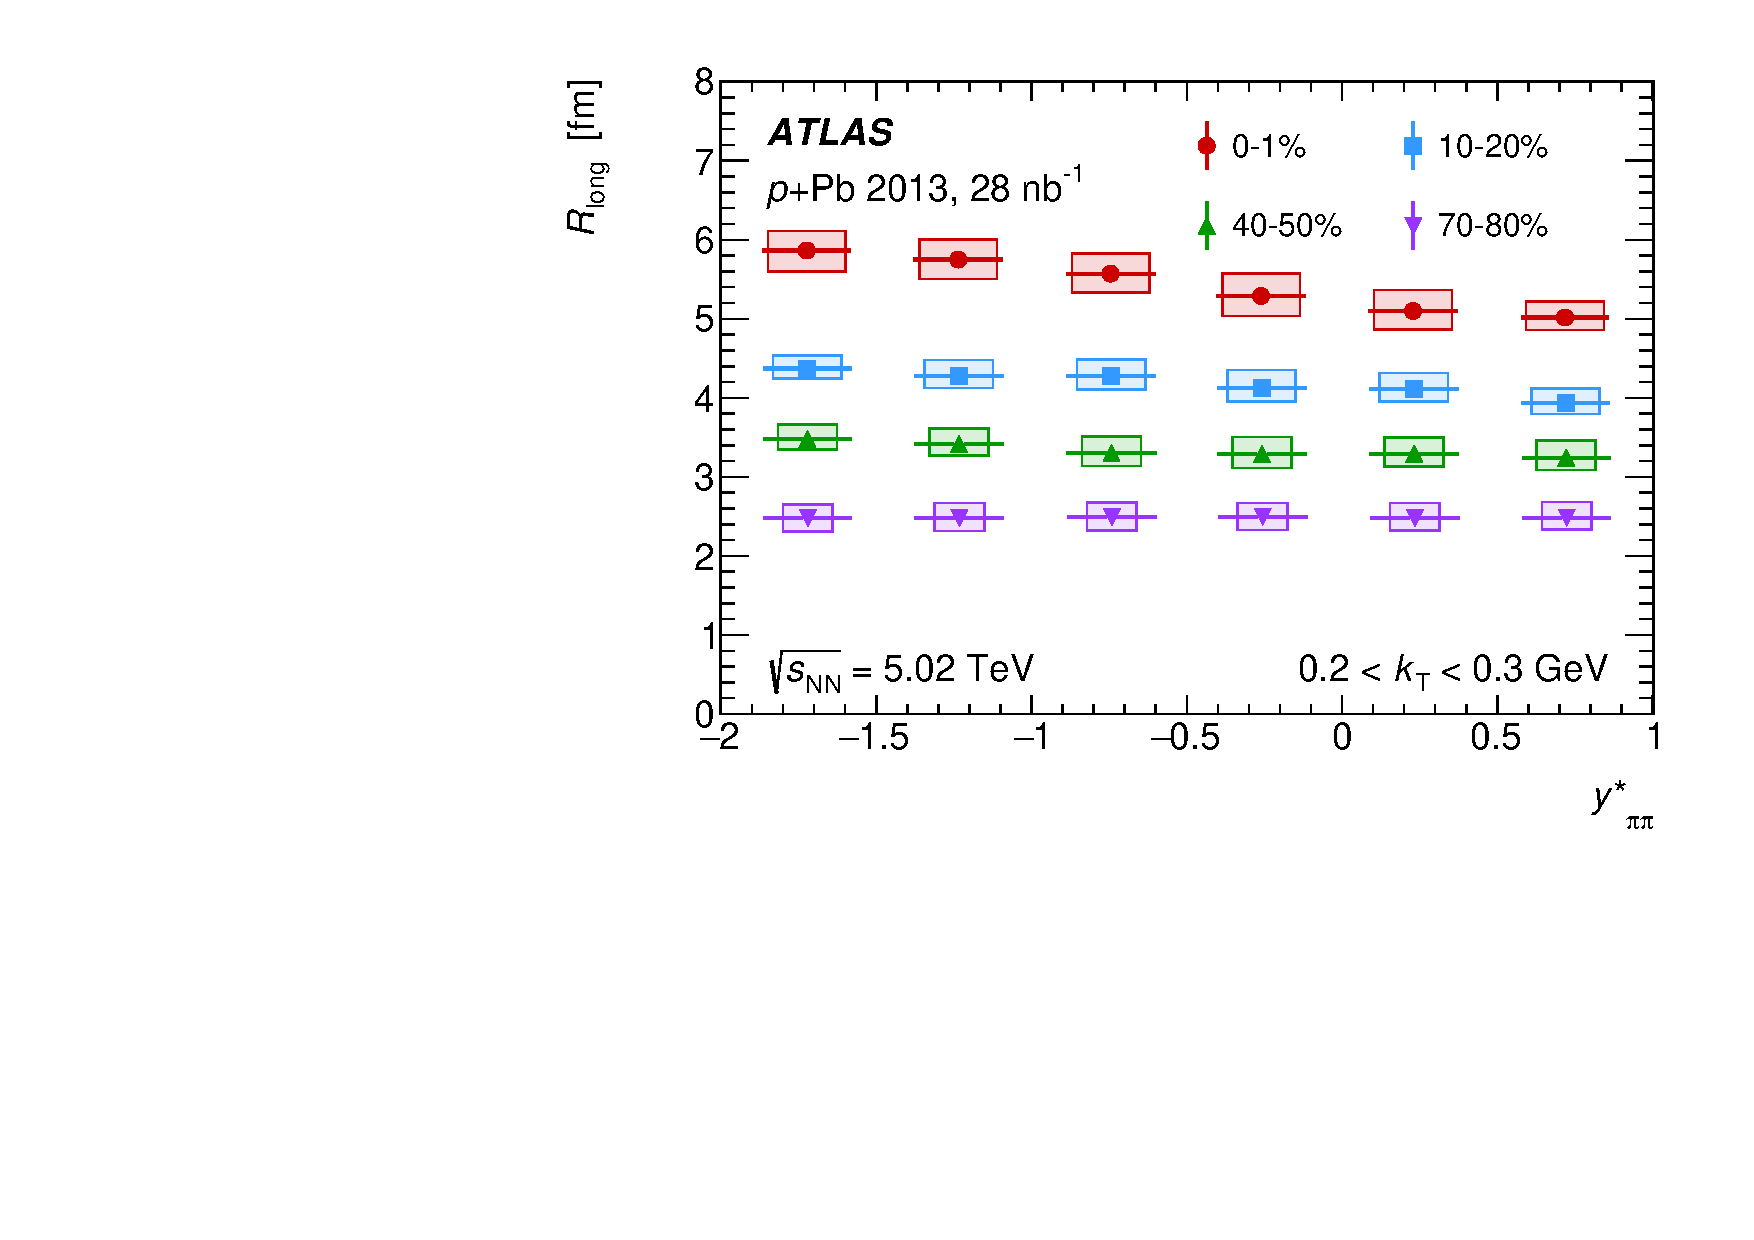
\includegraphics[width=.49\linewidth]{canqosl_Rlong_vs_kys.pdf}
\caption{Exponential fit results for 3D source radius, \Rlong, as a function of pair transverse momentum, \kt, (left) and rapidity, \kys (right). Four non-adjacent centrality intervals are shown. The vertical size of each box represents the quadrature sum of the systematic uncertainties described in \cref{sec:systematics}, and statistical uncertainties are shown with vertical lines. The horizontal positions of the points are the average \kt or \kys in each interval, and the horizontal lines indicate the standard deviation of \kt or \kys. The widths of the boxes differ among centrality intervals only for visual clarity.}
\label{fig:results_Rlong}
\end{figure}

The 3D radii are also shown as a function of the cube root of both average event multiplicity and local density
in \cref{fig:results_Rout_mult,fig:results_Rside_mult,fig:results_Rlong_mult}.
These plots demonstrate the relationship between the size and the density of the source at freeze-out.
All of the radii are seen to be very strongly correlated with the local density.
The scaling of the radii is not far from being linear with the cube root of multiplicity.
This behavior is qualitatively similar to the scaling of \Rinv with \avgdNdeta in \cref{fig:results_Rinv_dndeta}.


\begin{figure}[ht]
\centering
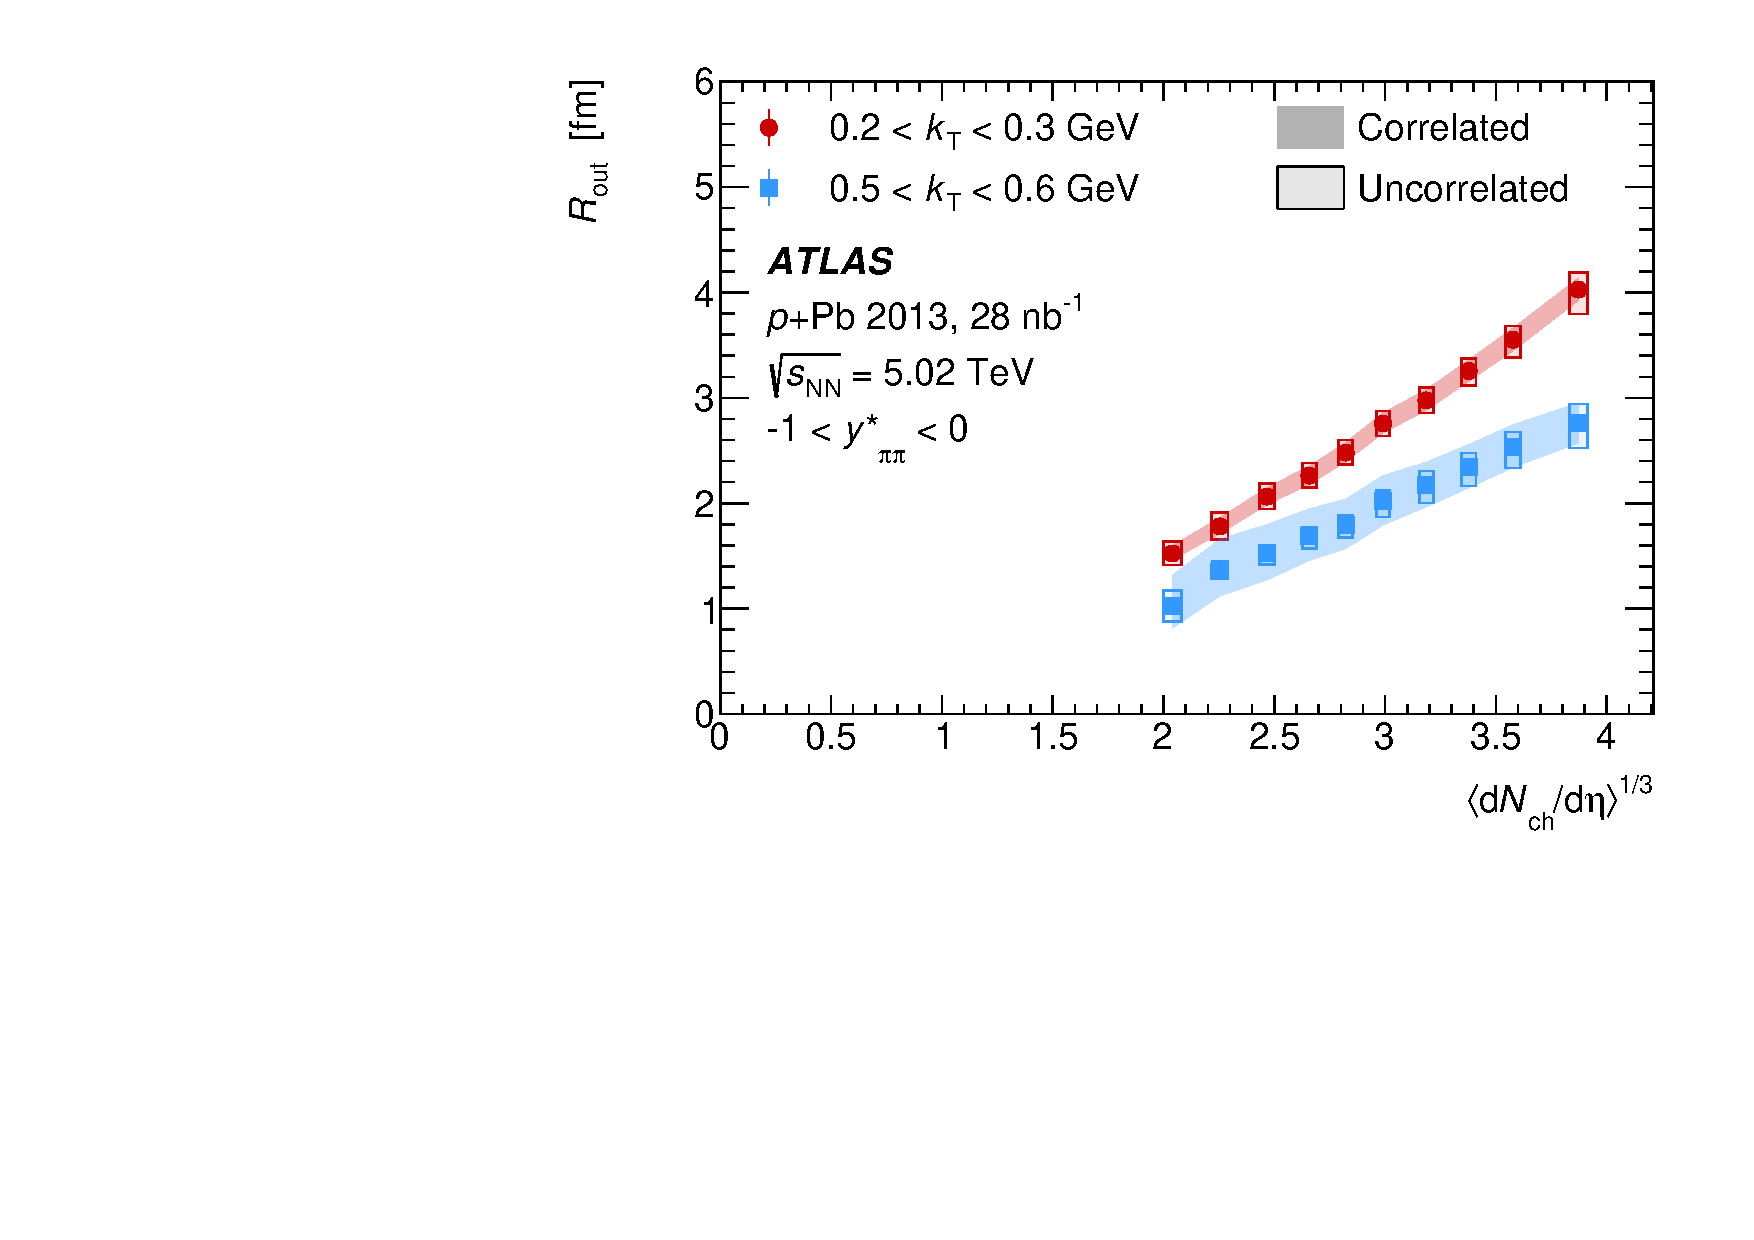
\includegraphics[width=0.49\linewidth]{canqosl_Rout_vs_avg_mult.pdf}
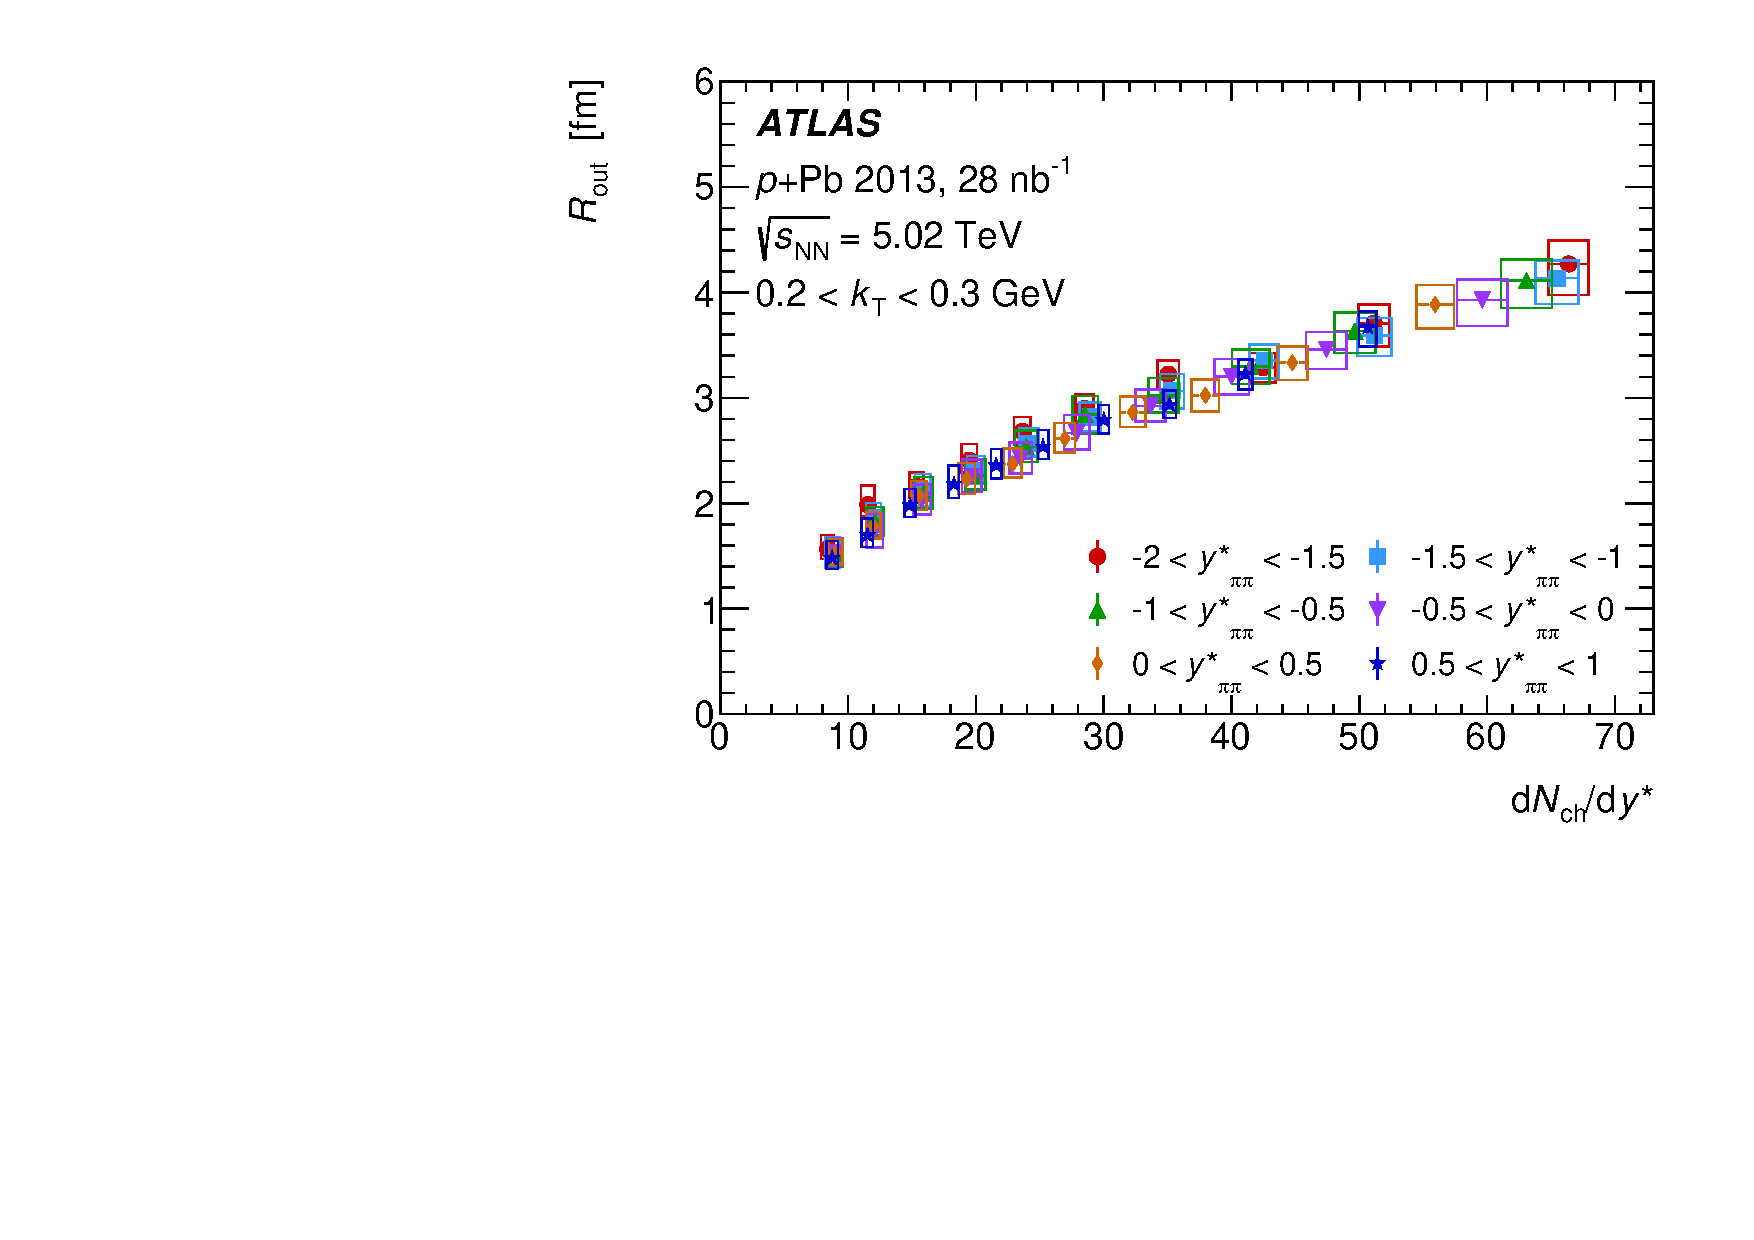
\includegraphics[width=0.49\linewidth]{canqosl_Rout_kt1_vs_mult.pdf}
\caption{Exponential fit results for \Rout as a function of (left) the cube root of average charged-particle multiplicity, $\avgdNdeta^{1/3}$, where the average is taken over $|\eta| < 1.5$ and (right) the local density, \dNdy, in intervals of \kys. In the left plot the systematic uncertainties from pion identification and from the generator and collision system components of the background amplitude are treated as correlated and shown as error bands, while the systematic uncertainties from charge asymmetry, \Reff, the rapidity variation of the jet fragmentation description, and two-particle reconstruction are treated as uncorrelated and indicated by the height of the boxes. The horizontal error bars indicate the systematic uncertainty from \avgdNdeta or \dNdy.}
\label{fig:results_Rout_mult}
\end{figure}

\begin{figure}[ht]
\centering
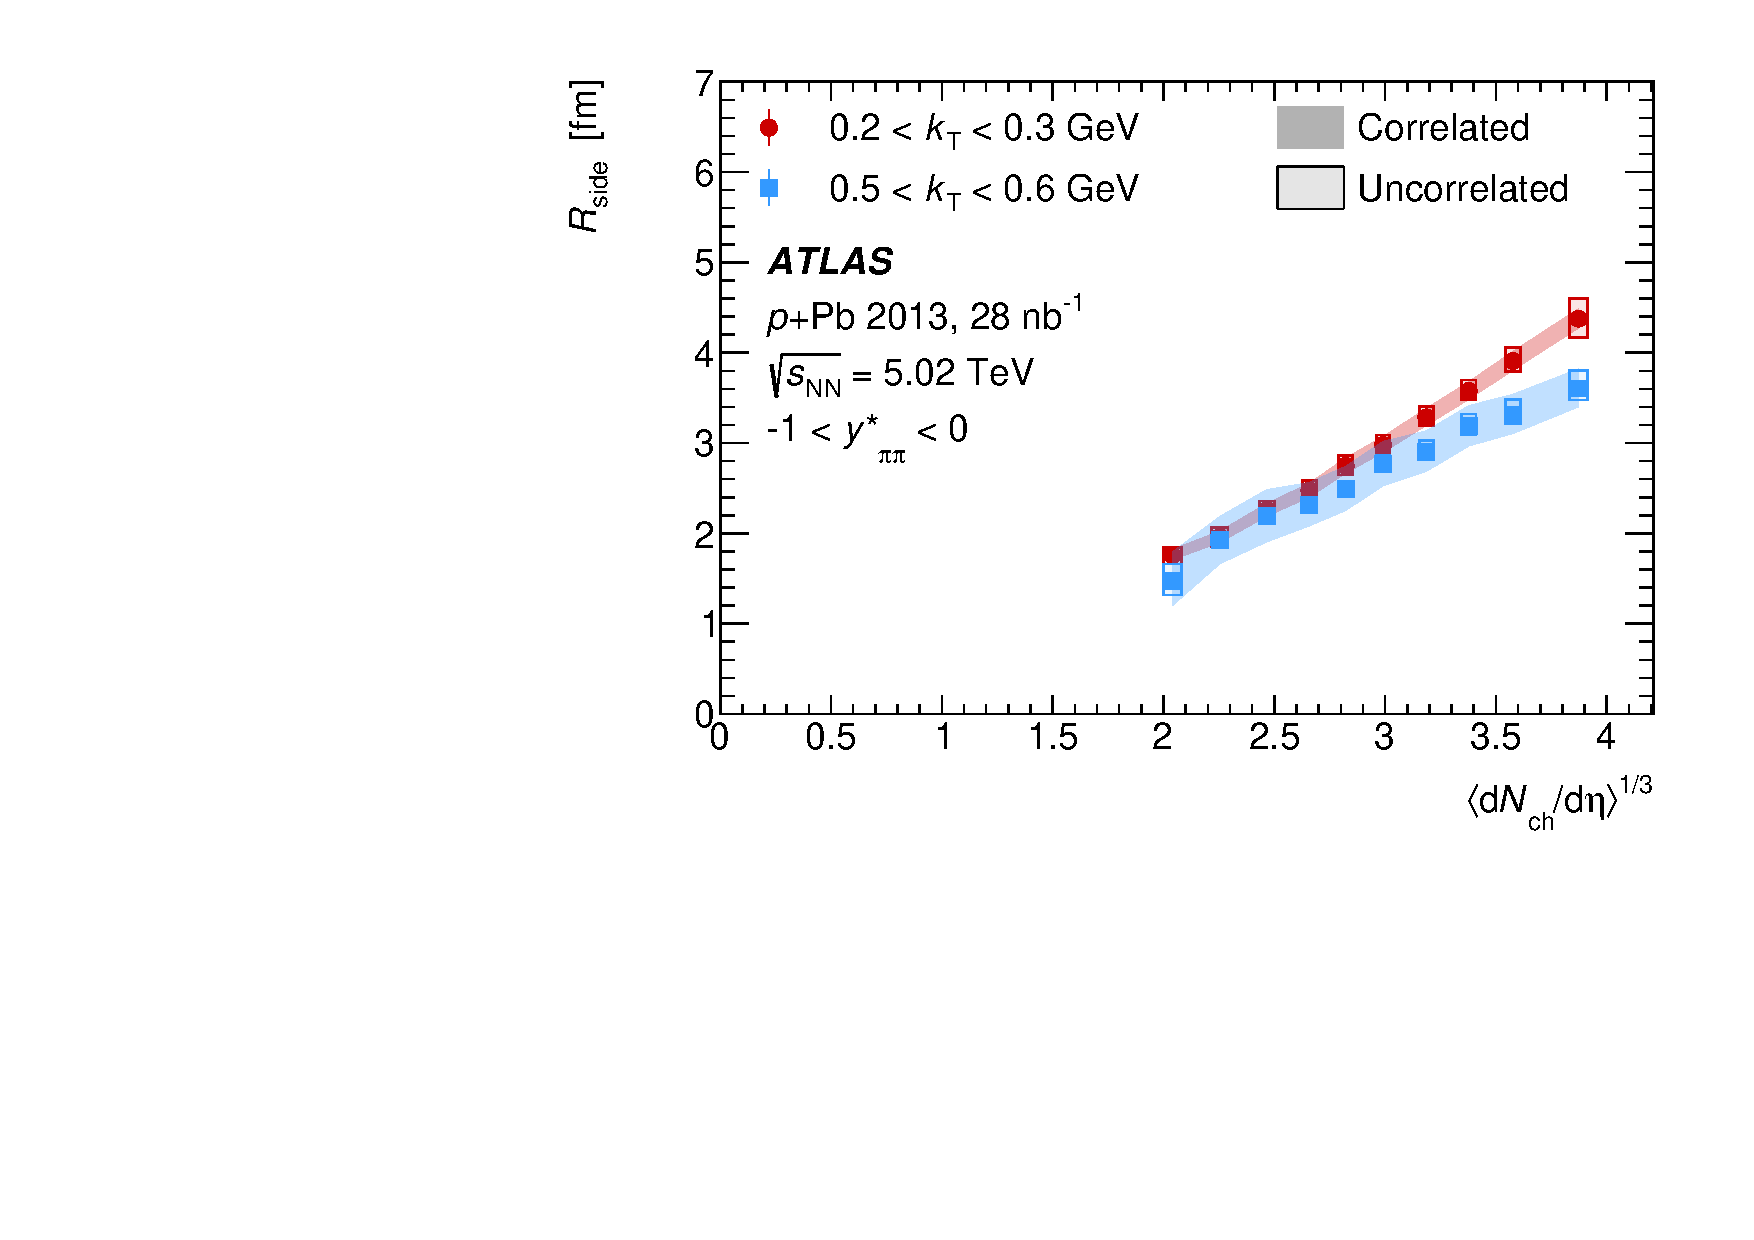
\includegraphics[width=0.49\linewidth]{canqosl_Rside_vs_avg_mult.pdf}
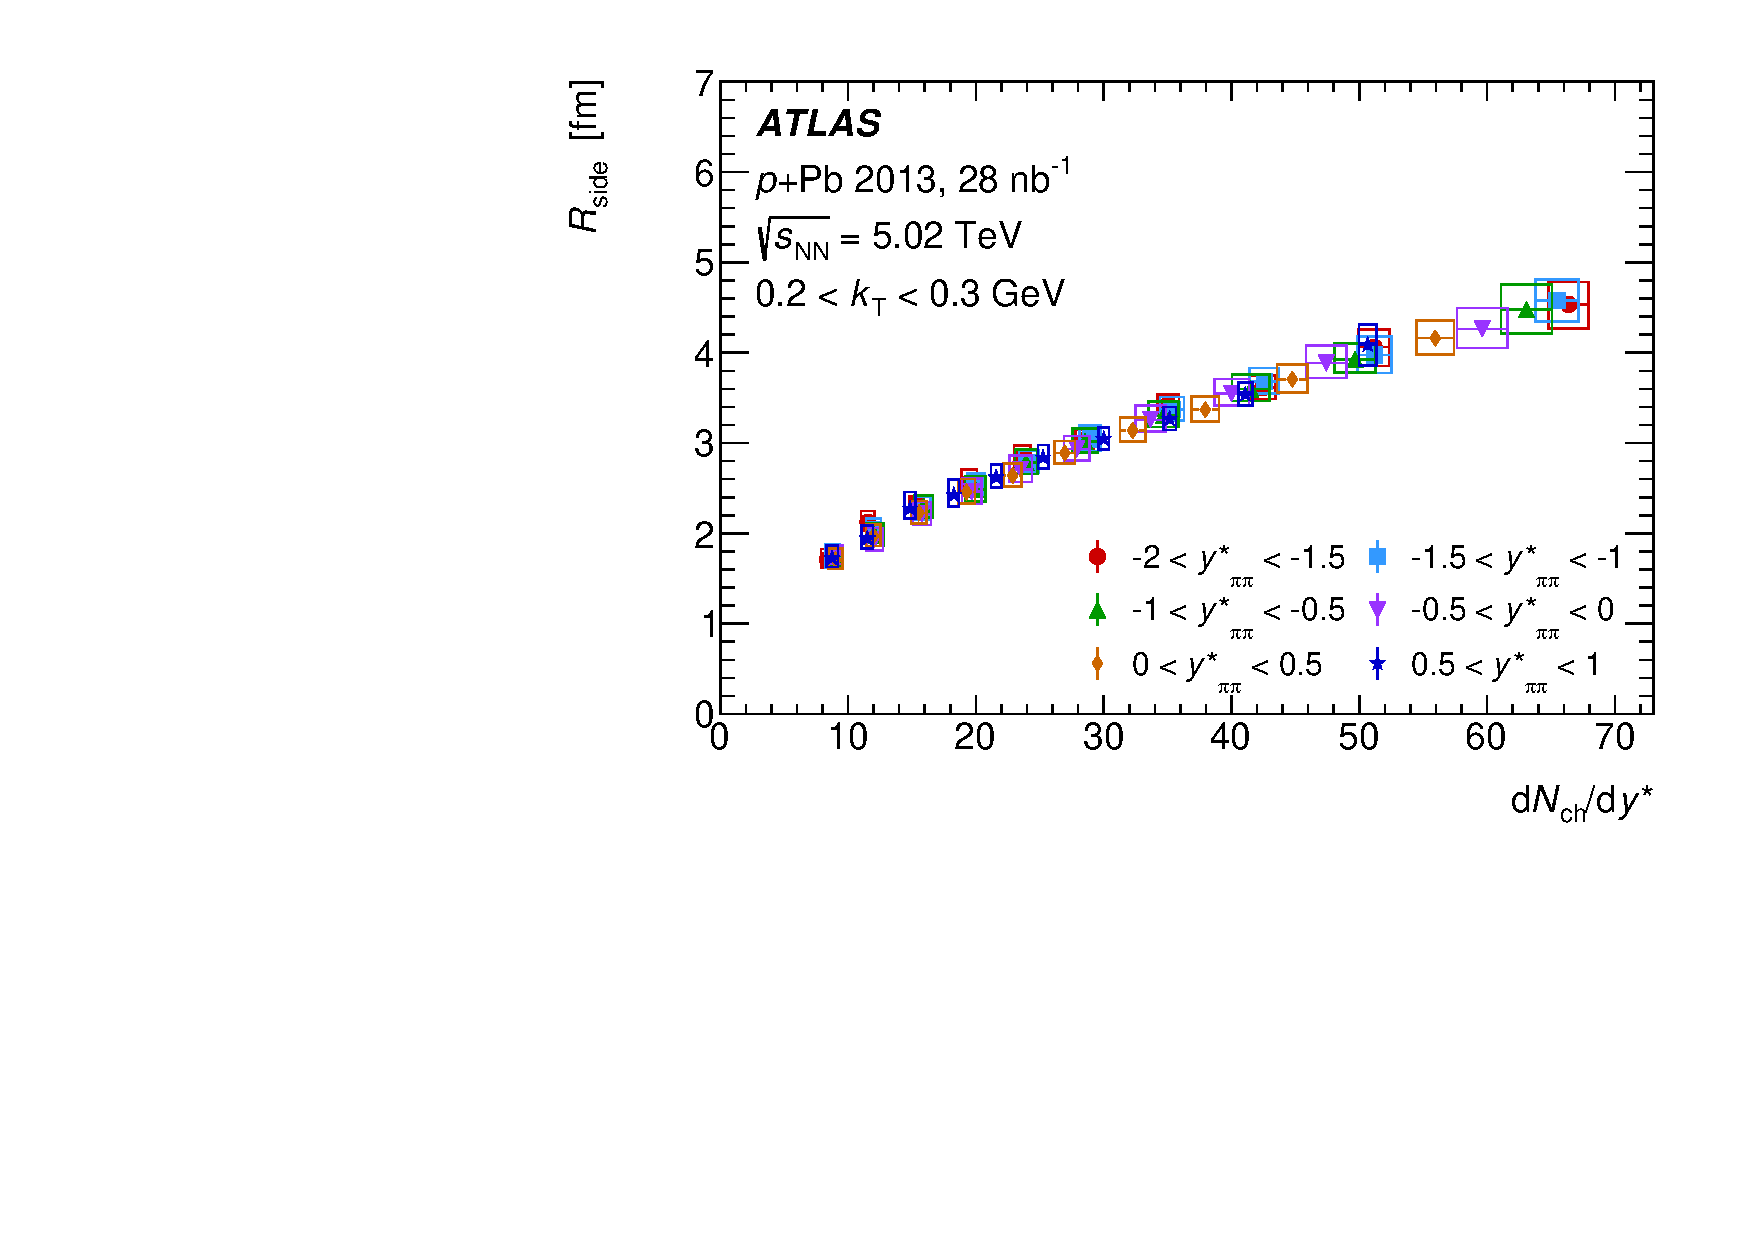
\includegraphics[width=0.49\linewidth]{canqosl_Rside_kt1_vs_mult.pdf}
\caption{Exponential fit results for \Rside as a function of (left) the cube root of average charged-particle multiplicity, $\avgdNdeta^{1/3}$, where the average is taken over $|\eta| < 1.5$ and (right) the local density, \dNdy, in intervals of \kys. In the left plot the systematic uncertainties from pion identification and from the generator and collision system components of the background amplitude are treated as correlated and shown as error bands, while the systematic uncertainties from charge asymmetry, \Reff, the rapidity variation of the jet fragmentation description, and two-particle reconstruction are treated as uncorrelated and indicated by the height of the boxes. The horizontal error bars indicate the systematic uncertainty from \avgdNdeta or \dNdy.}
\label{fig:results_Rside_mult}
\end{figure}

\begin{figure}[ht]
\centering
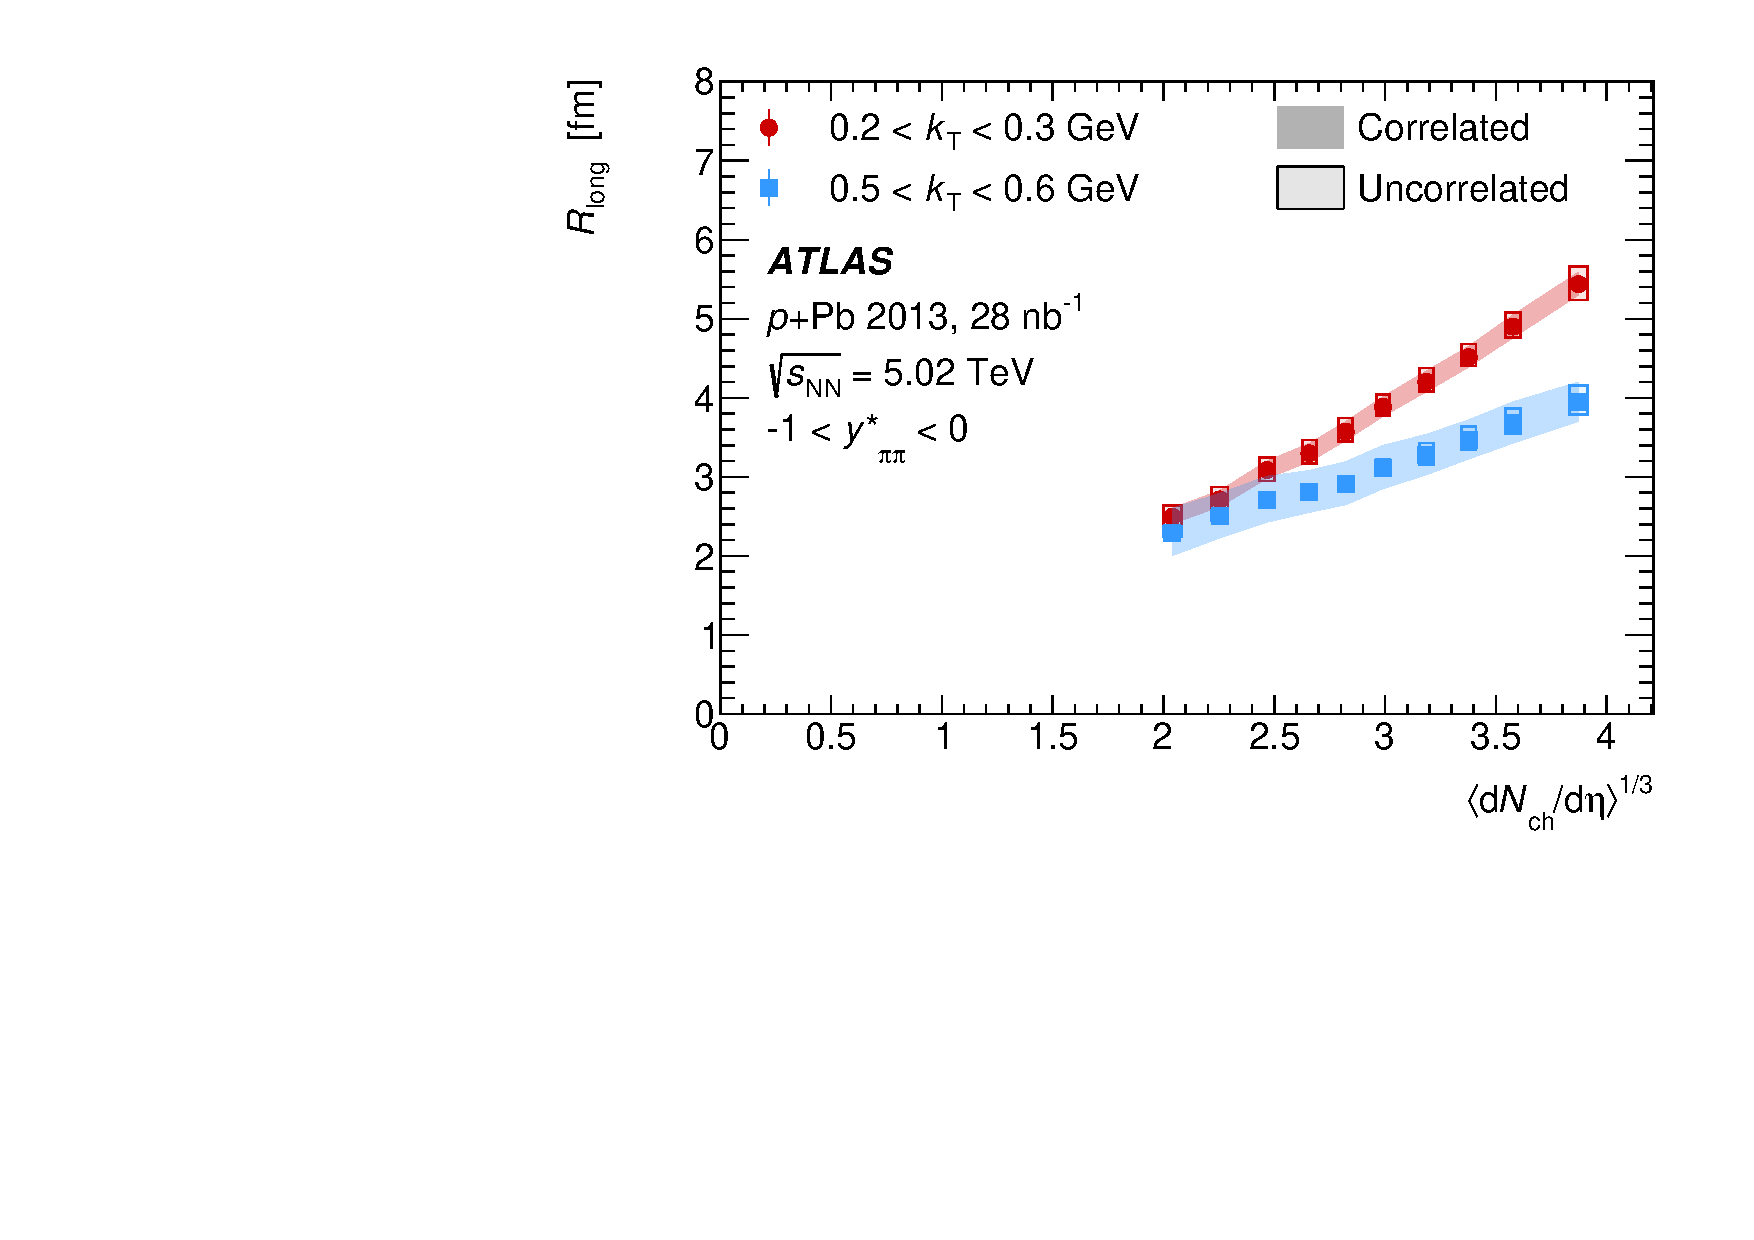
\includegraphics[width=0.49\linewidth]{canqosl_Rlong_vs_avg_mult.pdf}
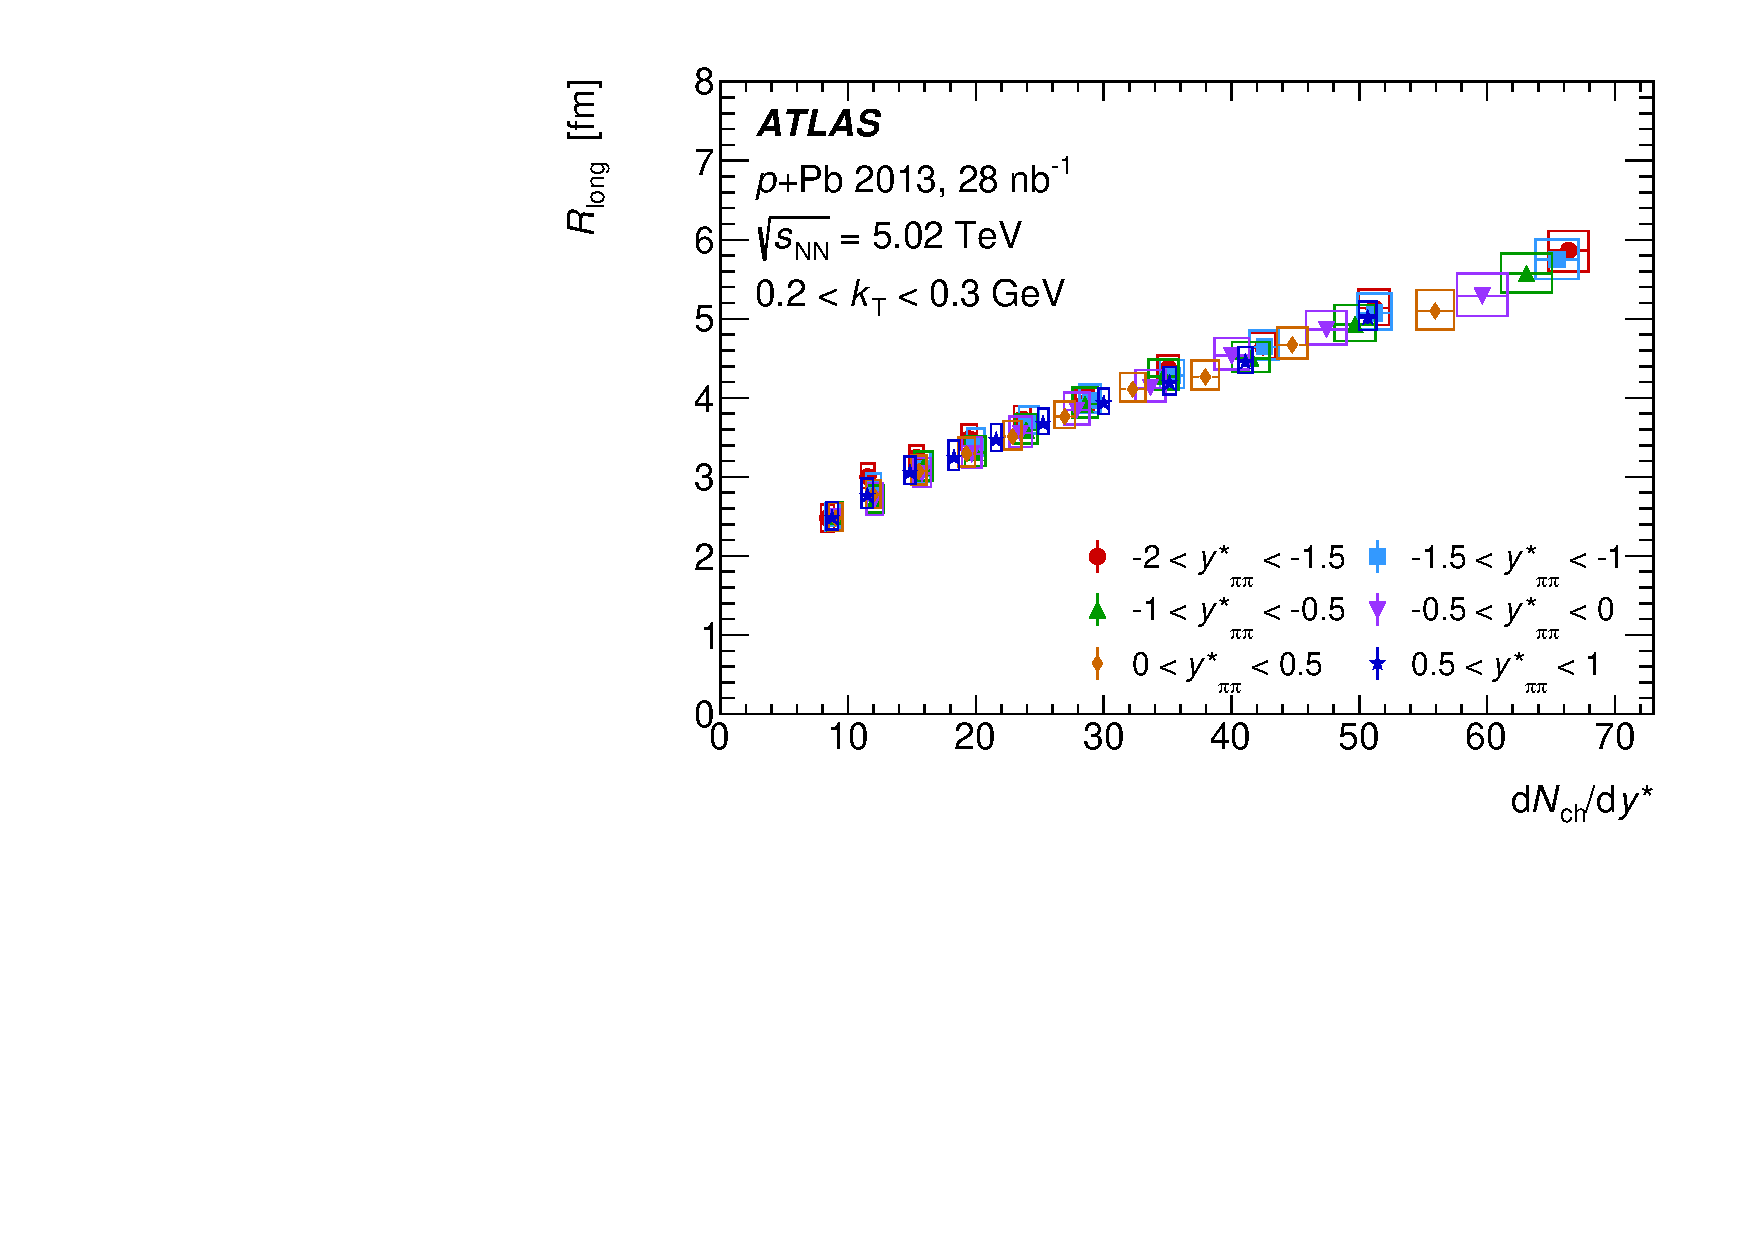
\includegraphics[width=0.49\linewidth]{canqosl_Rlong_kt1_vs_mult.pdf}
\caption{Exponential fit results for \Rlong as a function of (left) the cube root of average charged-particle multiplicity, $\avgdNdeta^{1/3}$, where the average is taken over $|\eta| < 1.5$  and (right) the local density, \dNdy, in intervals of \kys. In the left plot the systematic uncertainties from pion identification and from the generator and collision system components of the background amplitude are treated as correlated and shown as error bands, while the systematic uncertainties from charge asymmetry, \Reff, the rapidity variation of the jet fragmentation description, and two-particle reconstruction are treated as uncorrelated and indicated by the height of the boxes. The horizontal error bars indicate the systematic uncertainty from \avgdNdeta or \dNdy.}
\label{fig:results_Rlong_mult}
\end{figure}

\FloatBarrier

\begin{figure}[ht]
\centering
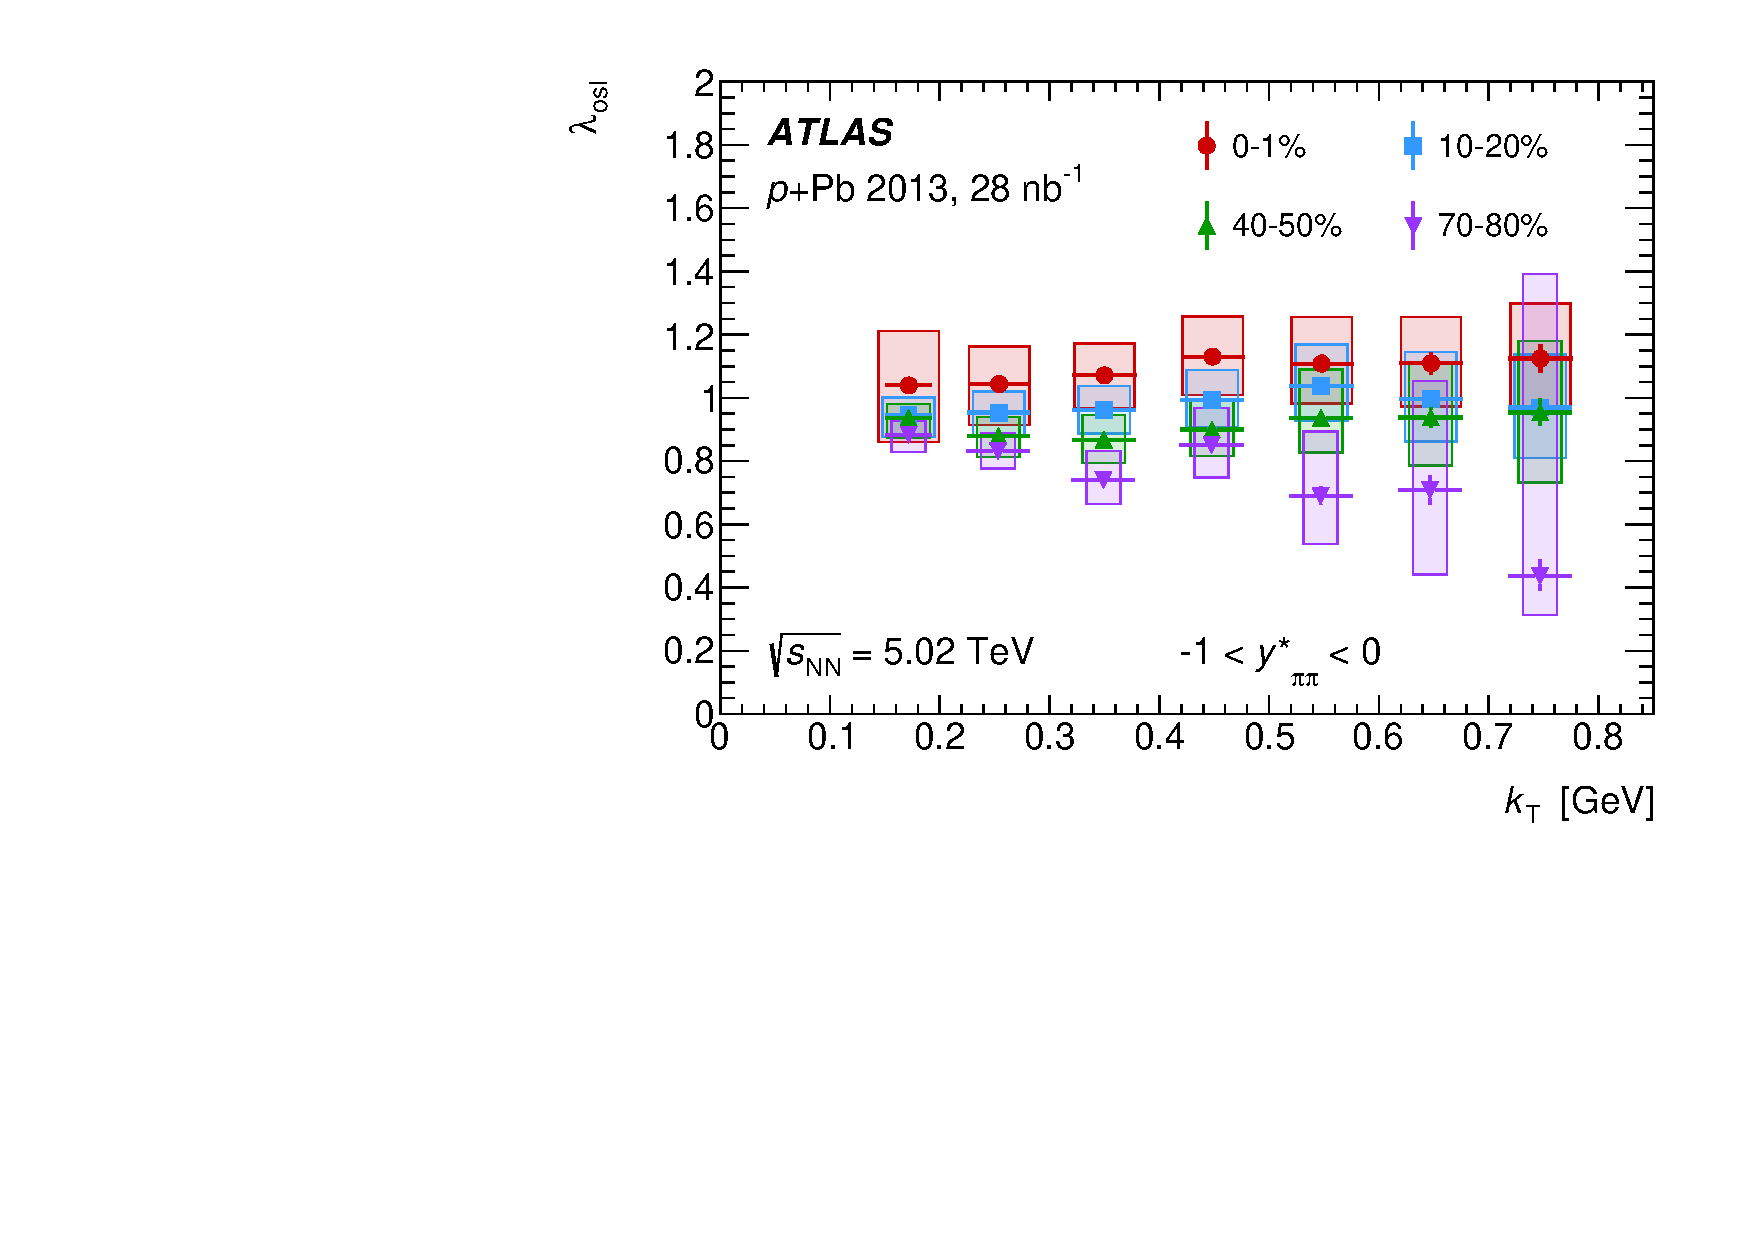
\includegraphics[width=0.49\linewidth]{canqosl_x_vs_kt.pdf}
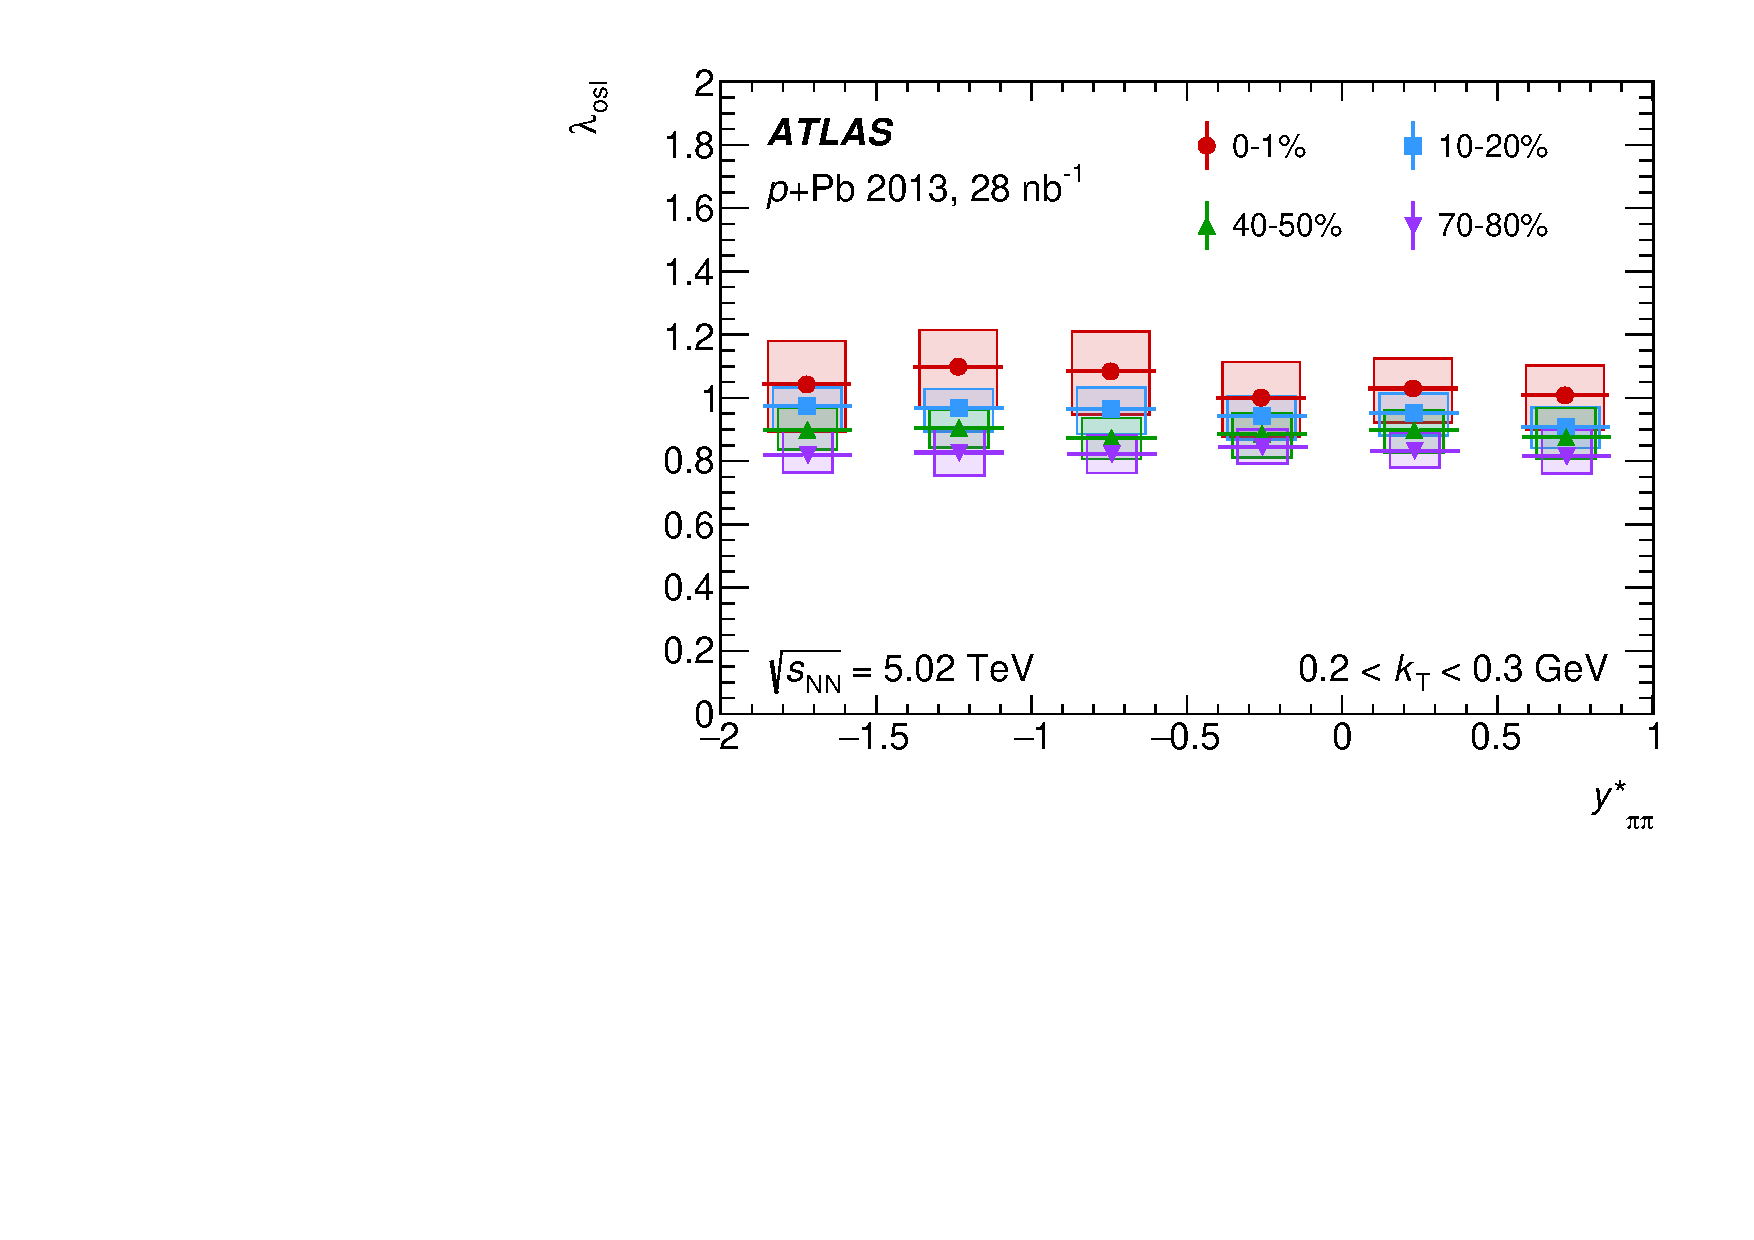
\includegraphics[width=0.49\linewidth]{canqosl_x_vs_kys.pdf}
\caption{The Bose-Einstein amplitude, \losl, as a function of pair transverse momentum, \kt, (left) and rapidity, \kys (right). Four non-adjacent centrality intervals are shown. The vertical size of each box represents the quadrature sum of the systematic uncertainties described in \cref{sec:systematics}, and statistical uncertainties are shown with vertical lines. The horizontal positions of the points are the average \kt or \kys in each interval, and the horizontal lines indicate the standard deviation of \kt or \kys. The widths of the boxes differ among centrality intervals only for visual clarity.}
\label{fig:results_qosl_x}
\end{figure}


\begin{figure}[ht]
\centering
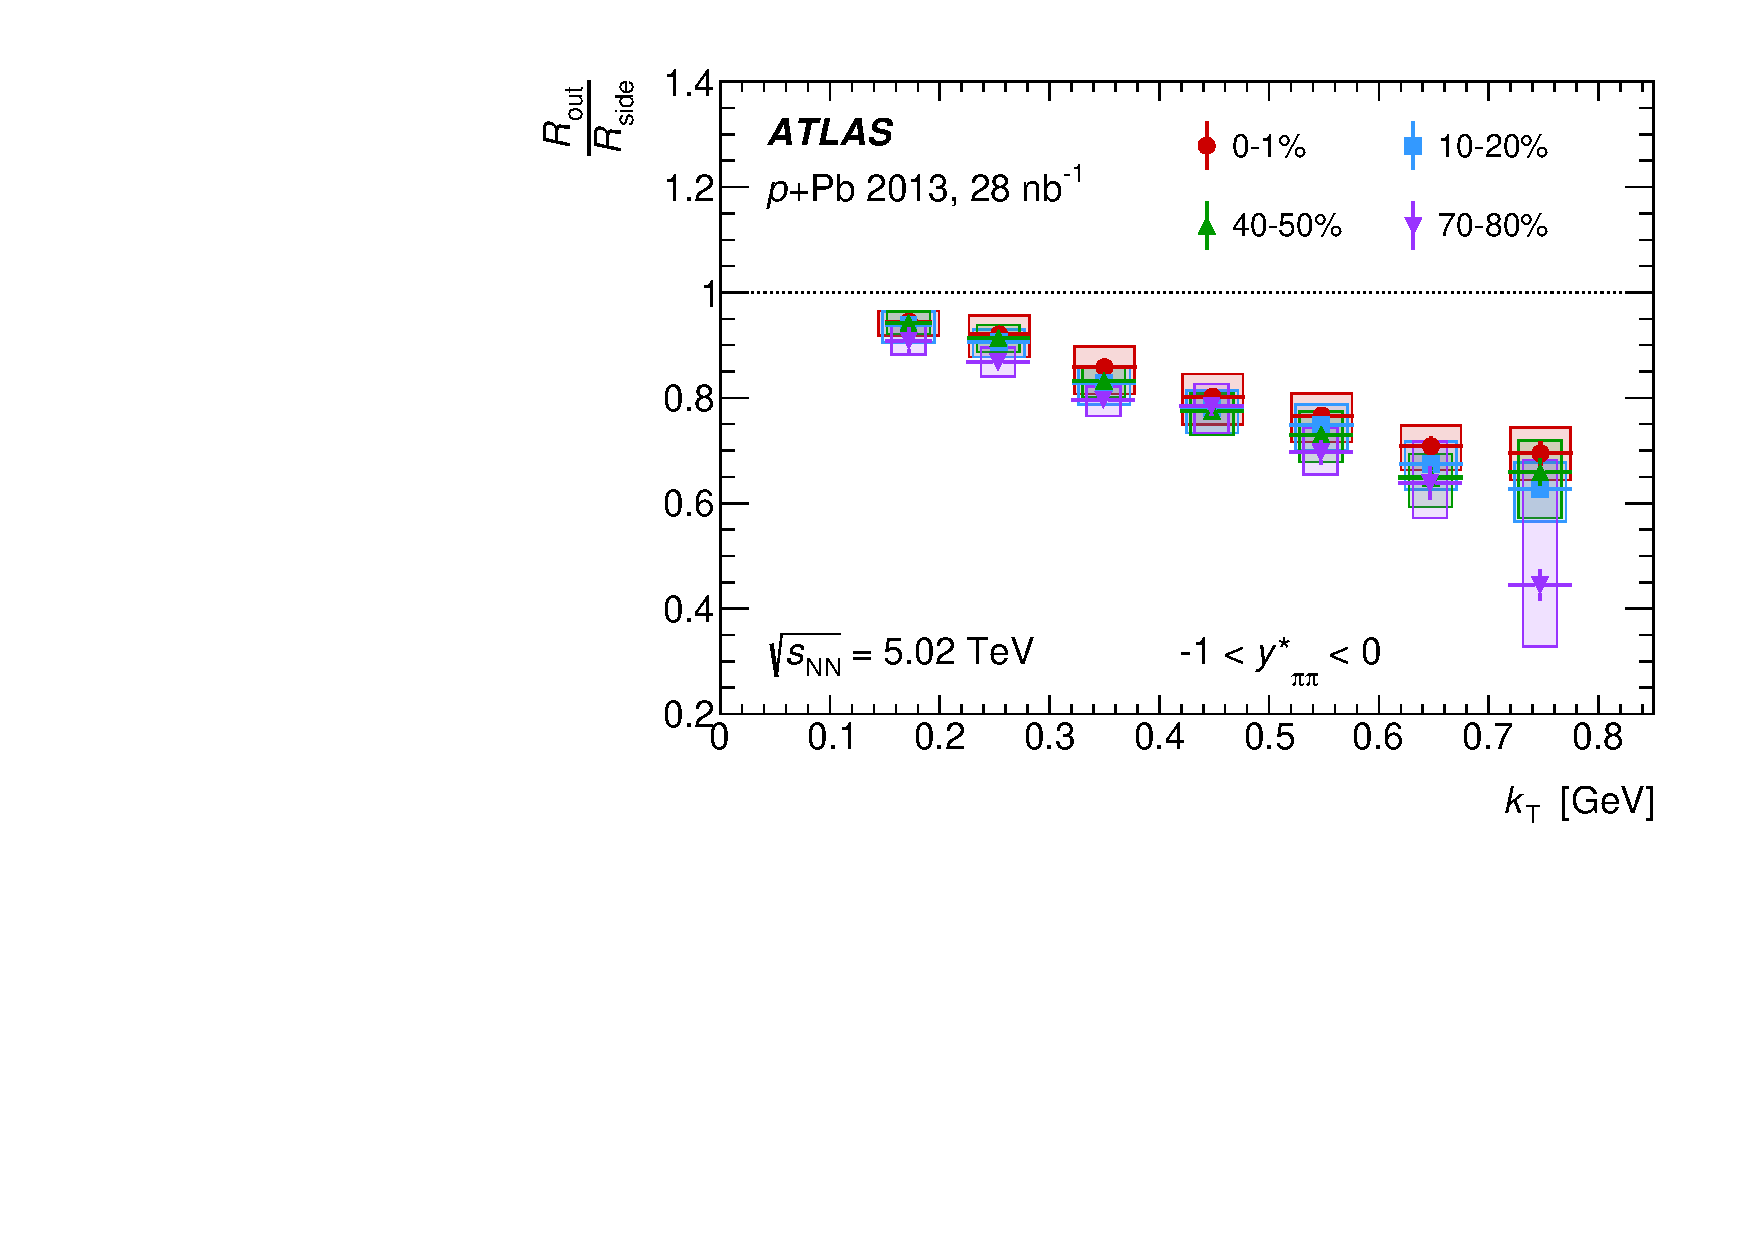
\includegraphics[width=0.49\linewidth]{canqosl_RoutOverRside_vs_kt.pdf}
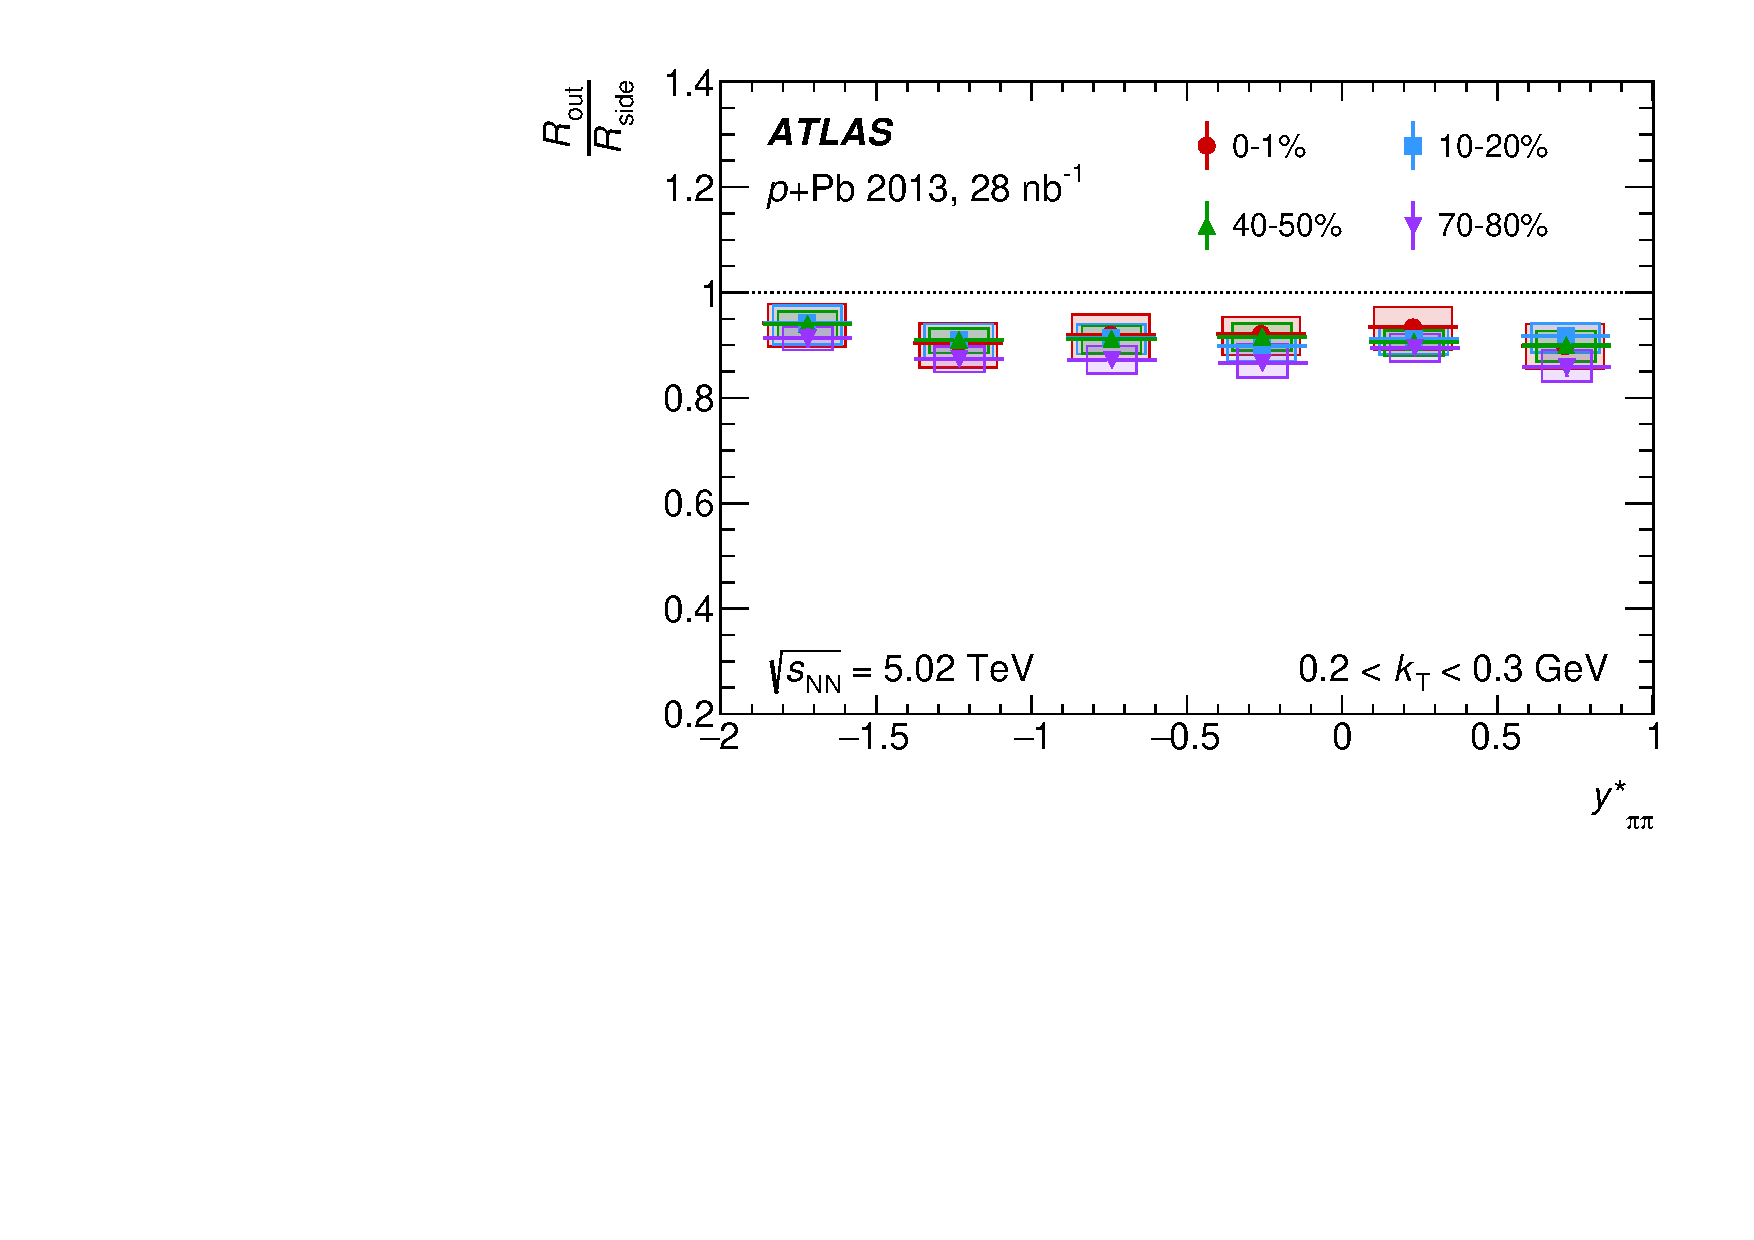
\includegraphics[width=0.49\linewidth]{canqosl_RoutOverRside_vs_kys.pdf}
\caption{The ratio of exponential radii $\Rout/\Rside$ as a function of pair transverse momentum, \kt, (left) and rapidity, \kys (right). Four non-adjacent centrality intervals are shown. The vertical size of each box represents the quadrature sum of the systematic uncertainties described in \cref{sec:systematics}, and statistical uncertainties are shown with vertical lines. The horizontal positions of the points are the average \kt or \kys in each interval, and the horizontal lines indicate the standard deviation of \kt or \kys. The widths of the boxes differ among centrality intervals only for visual clarity.}
\label{fig:results_RoutOverRside_kt}
\end{figure}

The Bose-Einstein amplitude in the 3D fits, \losl, is shown in \cref{fig:results_qosl_x} as a function of \kt and \kys. Like the invariant amplitude, at low \kt it is larger for central events than for peripheral ones. The three-dimensional amplitude does not decrease significantly with rising \kt as the invariant amplitude does, except in the most peripheral events. The 3D amplitude also exhibits no significant variation over rapidity.

The ratio $\Rout/\Rside$ (\cref{fig:results_RoutOverRside_kt}) is often studied because in models with radial flow, \Rout includes components of the source's lifetime but \Rside does not (see, for instance, the discussion in \Ref{\cite{Lisa:2005dd}}).
A value of $\Rout/\Rside$ less than one is observed and it decreases with increasing \kt.
The ratio is observed to be the same in different centrality intervals within uncertainties.
As explained in \Ref{\cite{Pratt:2008qv}}, several improvements to naive hydrodynamic models---primarily pre-thermal acceleration, a stiffer equation of state, and shear viscosity---all result in more sudden emission.
This implies that a value of $\Rout/\Rside \lesssim 1$ does not necessarily rule out collective behavior.

\FloatBarrier

\begin{figure}[ht]
\centering
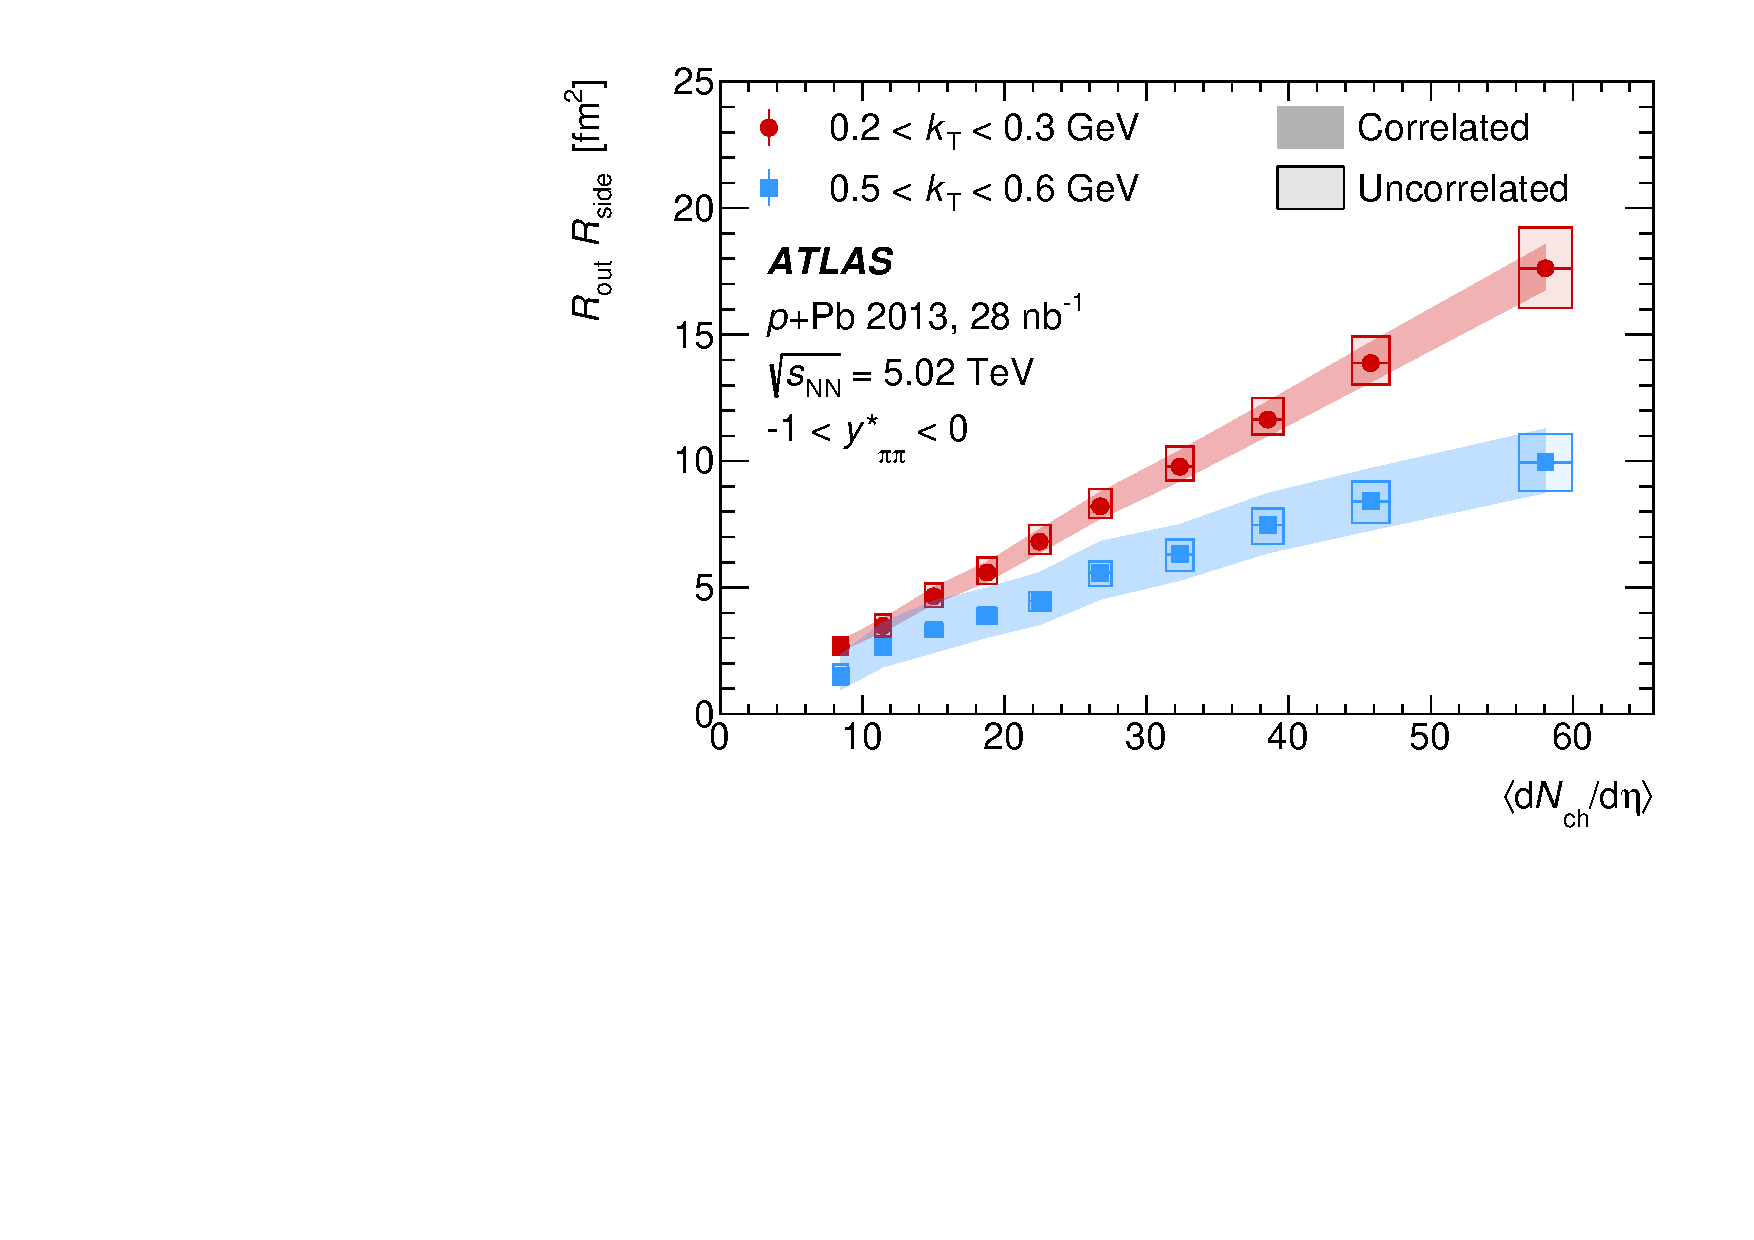
\includegraphics[width=0.49\linewidth]{canqosl_detRt_vs_avg_mult.pdf}
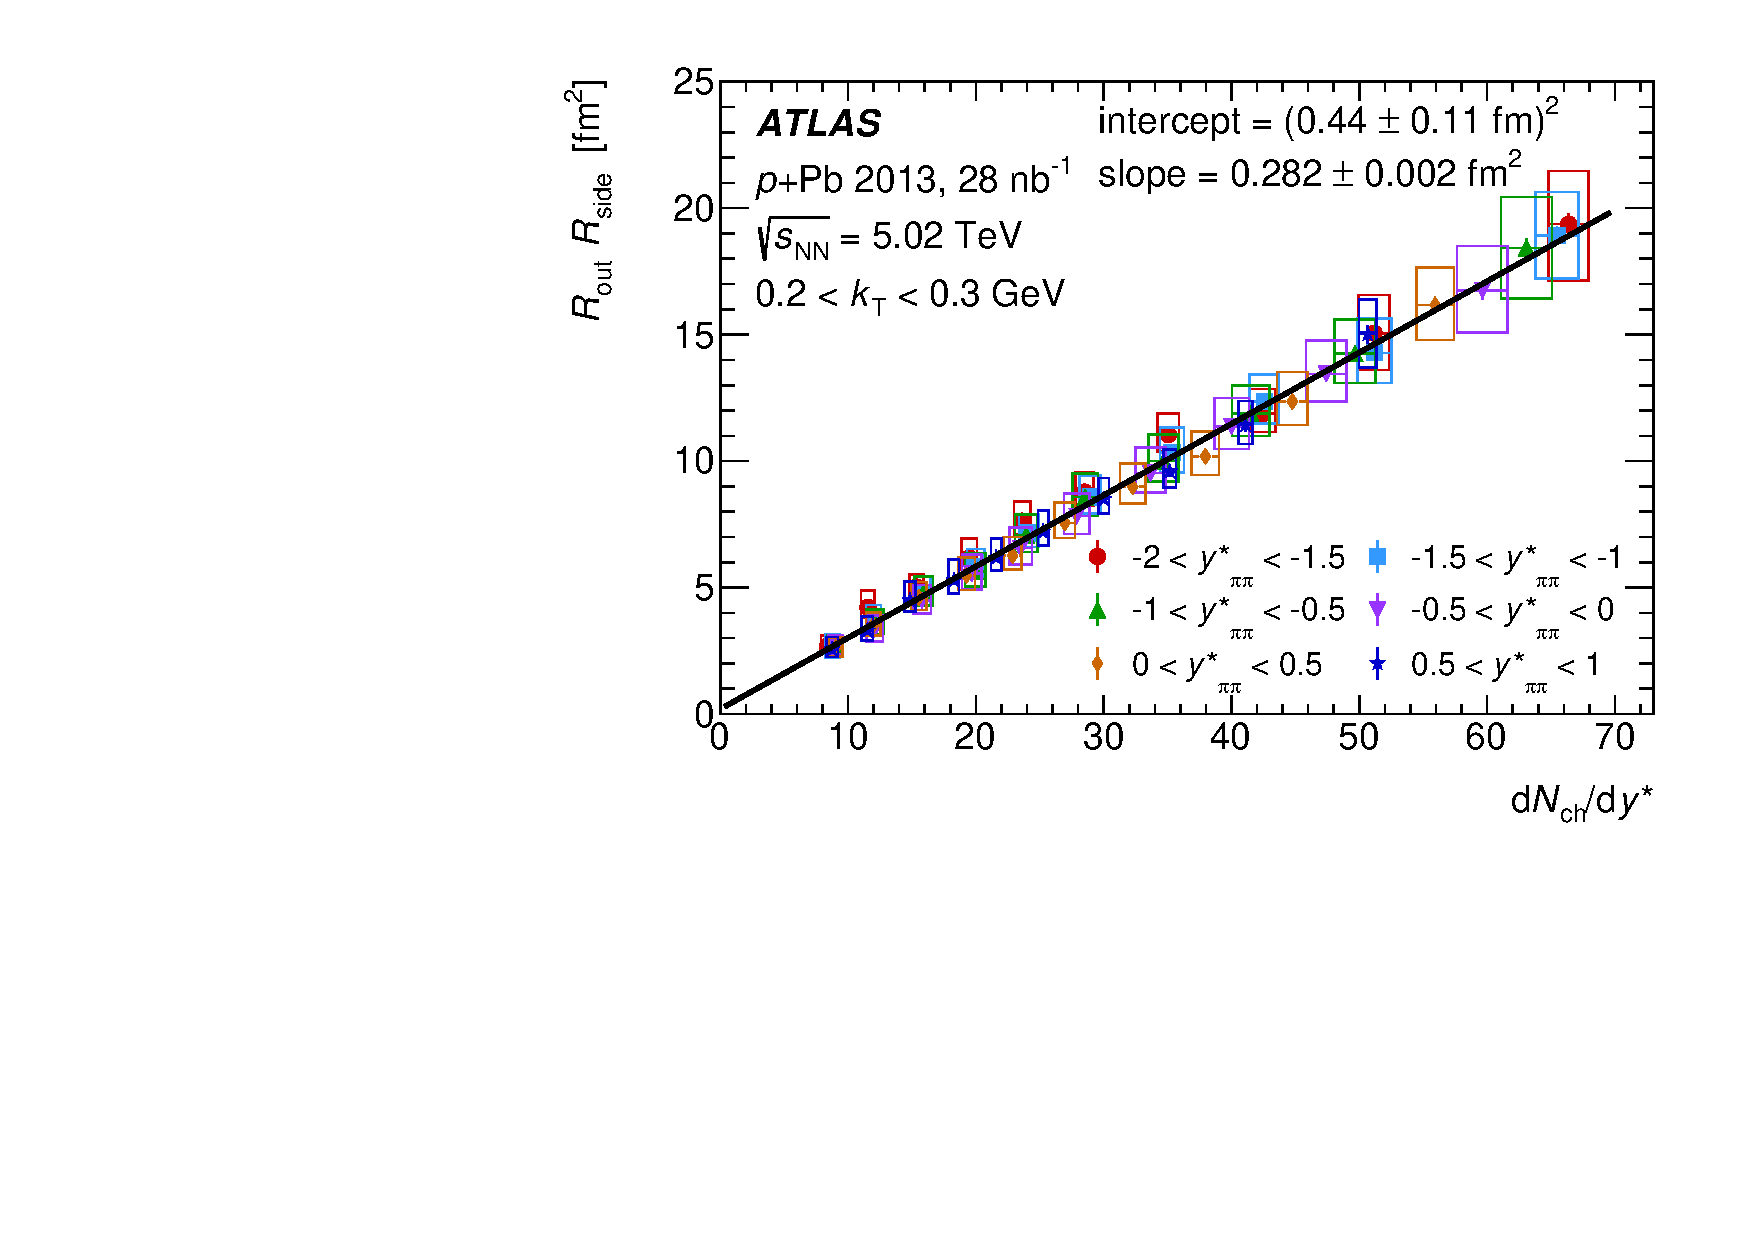
\includegraphics[width=0.49\linewidth]{canqosl_detRt_kt1_vs_mult.pdf}
\caption{The transverse area scale, $\Rout\Rside$, plotted against the average multiplicity, \avgdNdeta, (left) and the local density, \dNdy, as a function of rapidity (right). The systematic uncertainties from pion identification and the generator and collision system components of the jet background description are treated as correlated and shown as error bands. The systematic uncertainties from charge asymmetry, \Reff, rapidity variation of the jet fragmentation, and two-particle track reconstruction effects are treated as uncorrelated and indicated by the height of the boxes. The horizontal error bars indicate the systematic uncertainty from \avgdNdeta or \dNdy. The slope and intercept of the best fit to the right-hand plot are shown with combined statistical and systematic uncertainties.}
\label{fig:results_detRt_mult}
\end{figure}

\begin{figure}[ht]
\centering
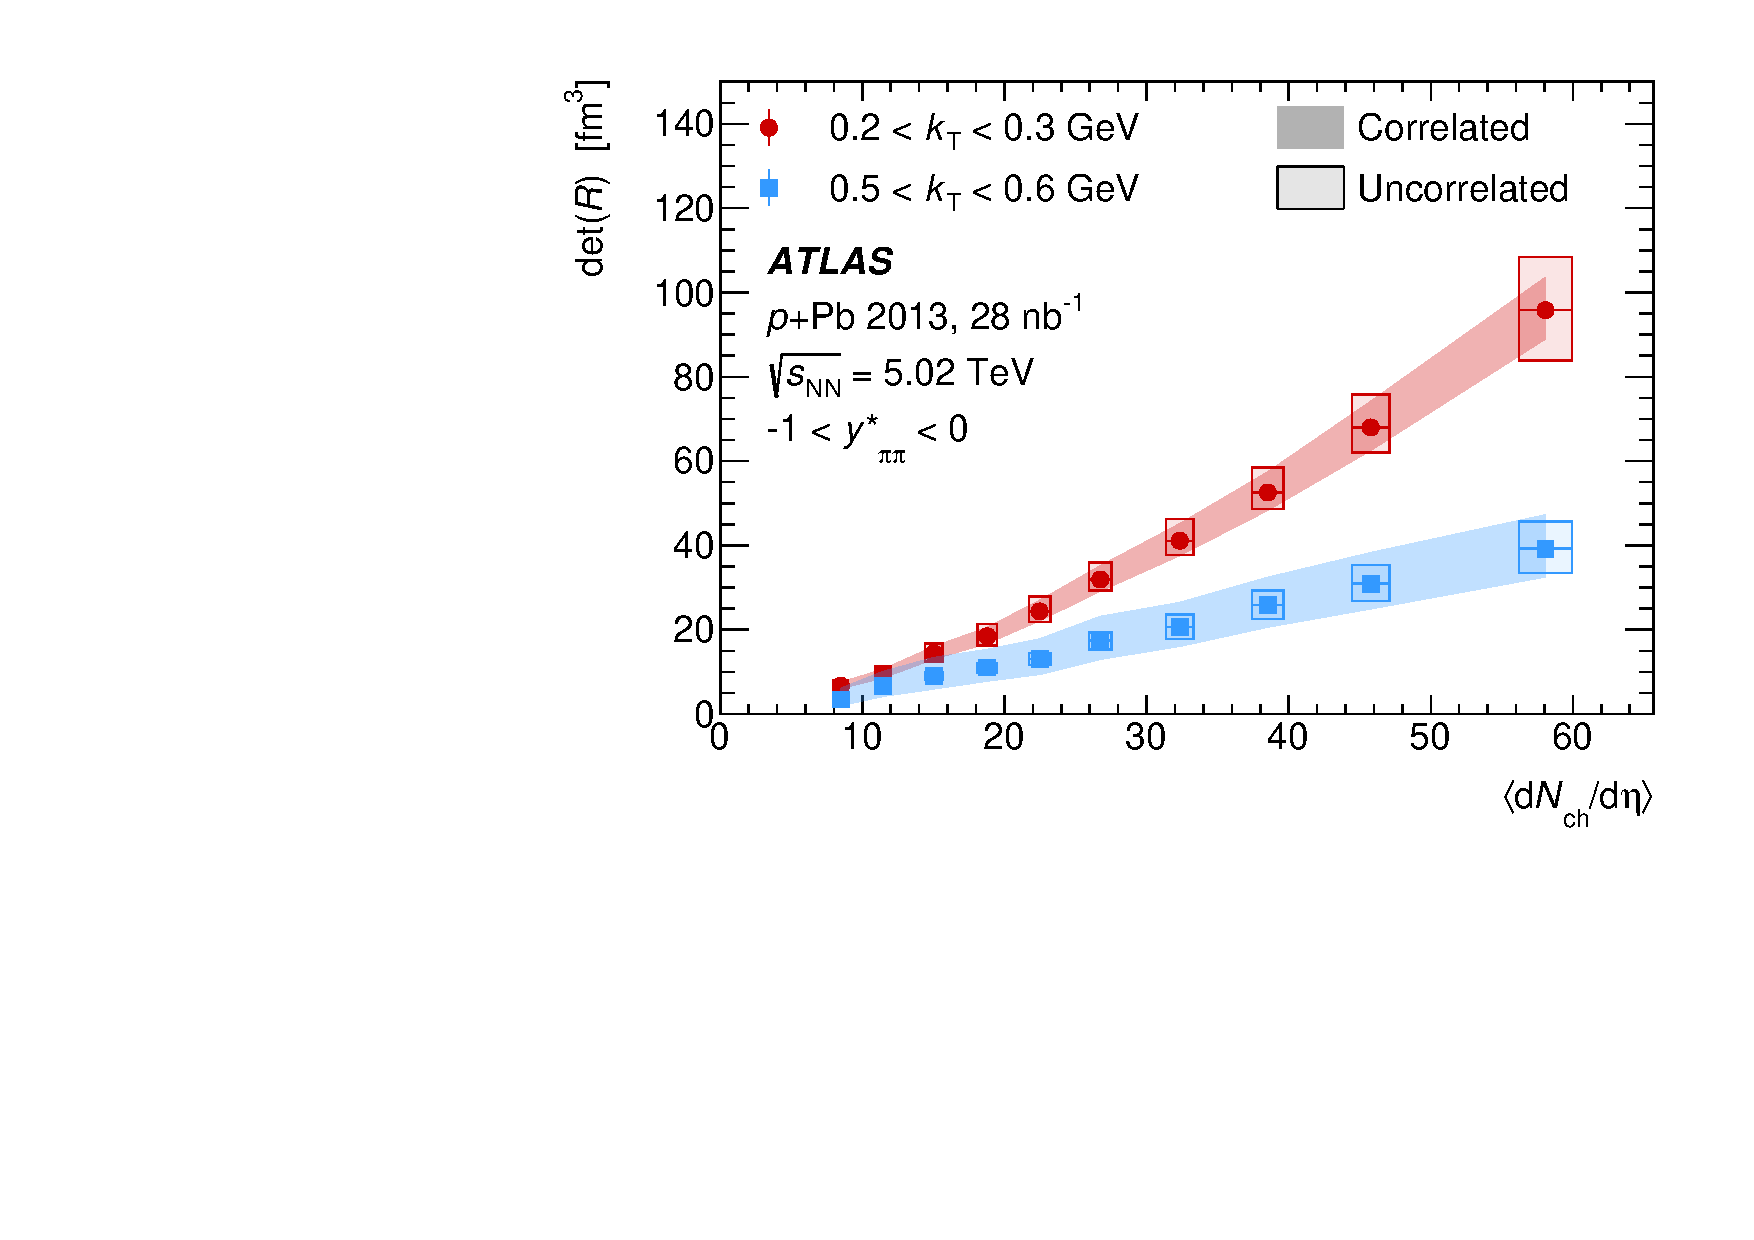
\includegraphics[width=0.49\linewidth]{canqosl_detR_vs_avg_mult.pdf}
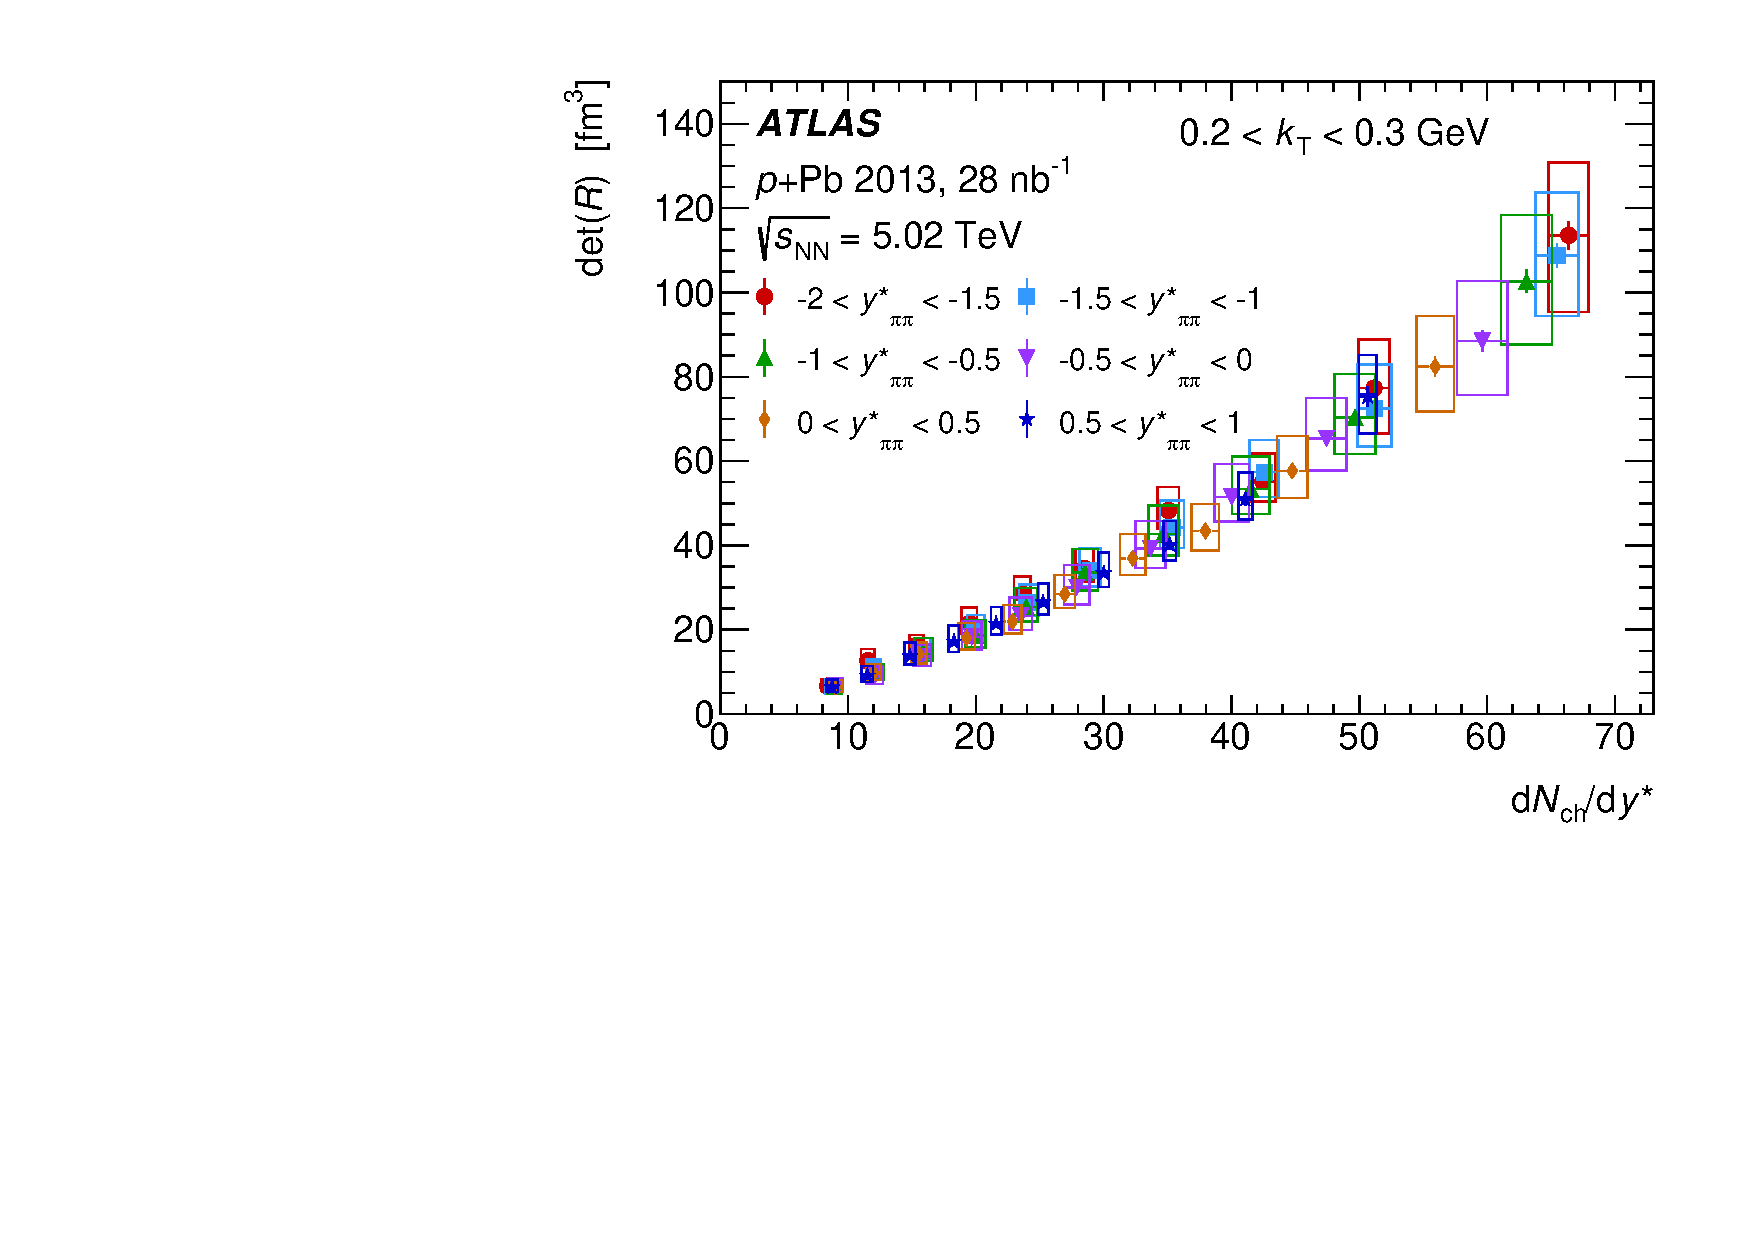
\includegraphics[width=0.49\linewidth]{canqosl_detR_kt1_vs_mult.pdf}
\caption{The volume scale, \detR, plotted against the average multiplicity, \avgdNdeta, (left) and the local density, \dNdy, as a function of rapidity (right). In the left plot, the systematic uncertainties from pion identification and the generator and collision system components of the jet background description are treated as correlated and shown as error bands, while those from charge asymmetry, \Reff, rapidity variation of the jet fragmentation, and two-particle track reconstruction effects are treated as uncorrelated and indicated by the height of the boxes. The widths of the boxes indicate the systematic uncertainty in \avgdNdeta or \dNdy.}
\label{fig:results_detR_dndeta}
\end{figure}

The transverse area scale $\Rout\Rside$ is shown in \cref{fig:results_detRt_mult} as a function of both event and local density. At lower \kt, the transverse area scales linearly with multiplicity over all centralities and rapidities. This result is consistent with a picture in which the longitudinal dynamics can be separated from the transverse particle production, and low-\kt particles freeze out at a constant transverse area density.


\begin{figure}[t]
\centering
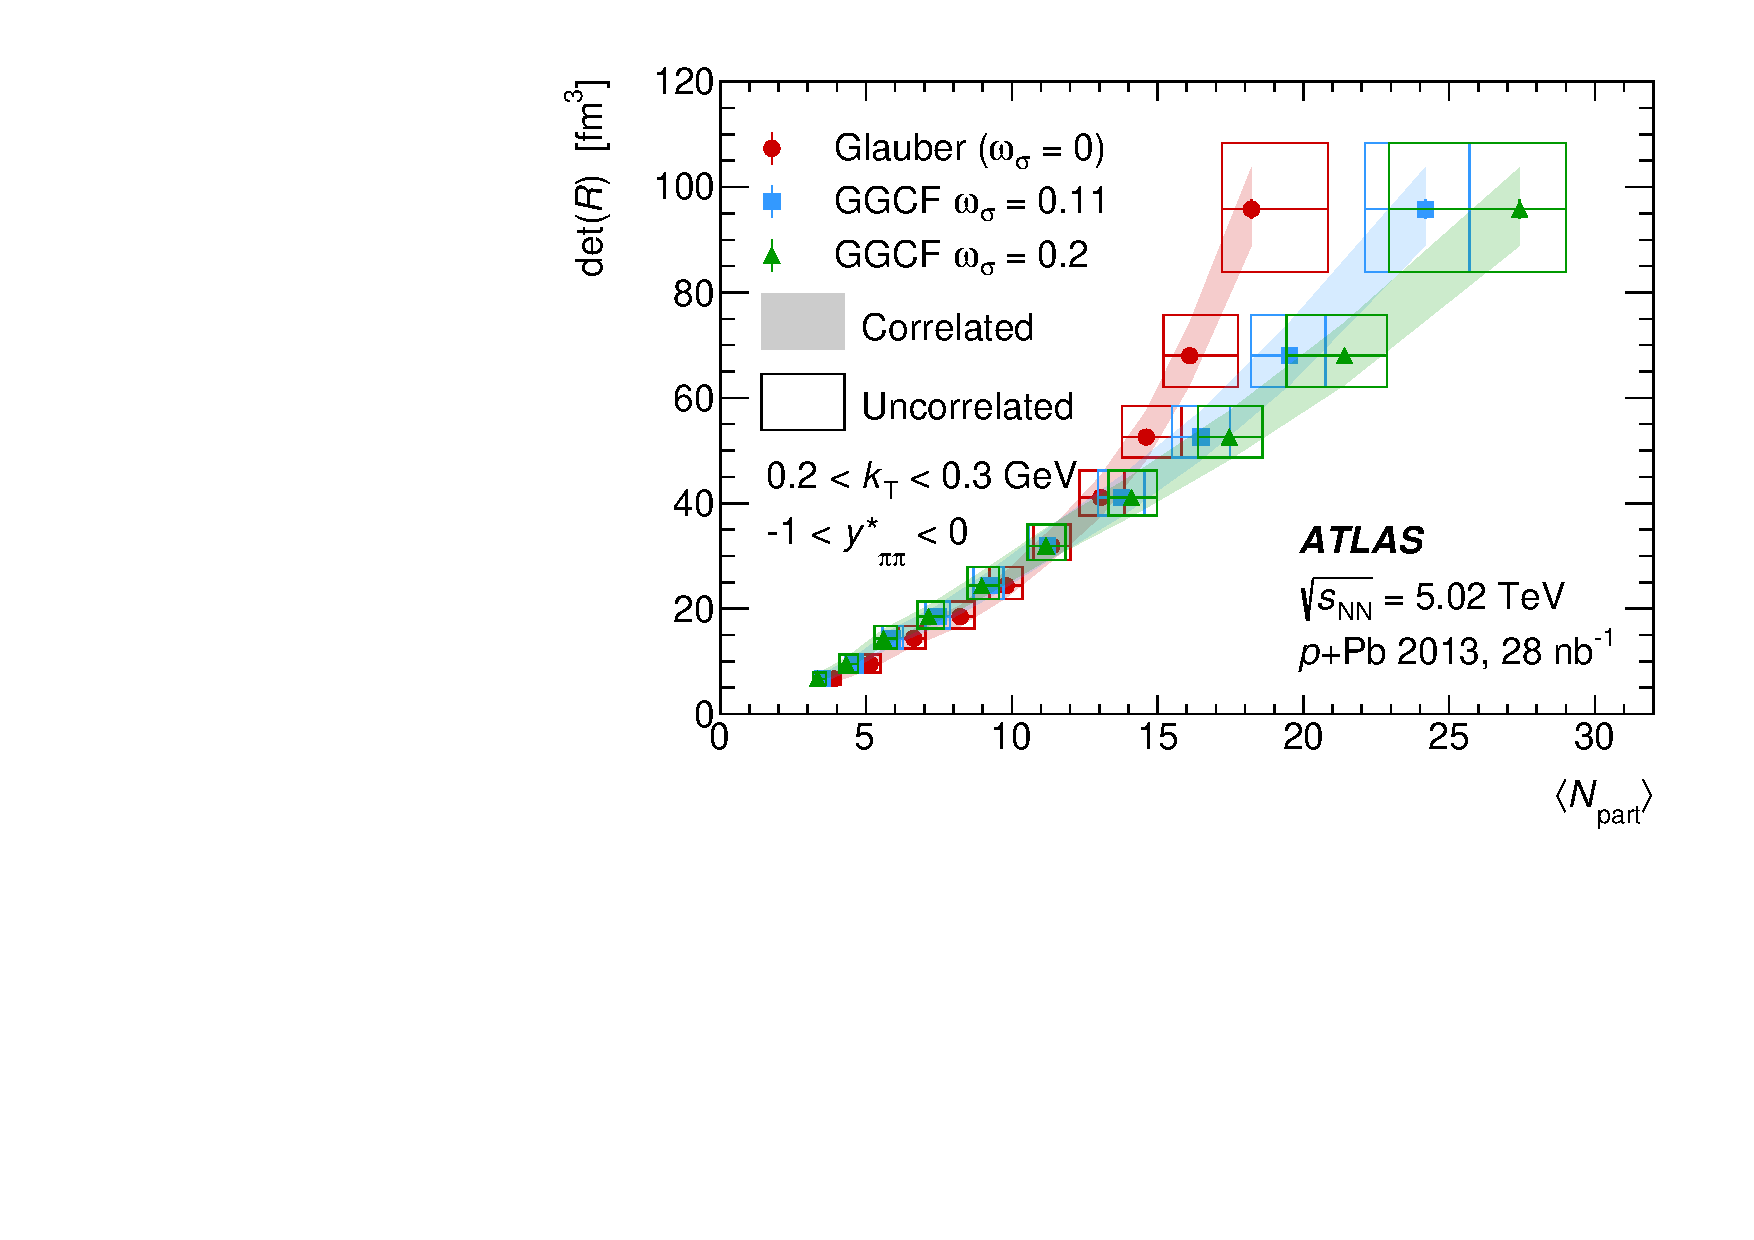
\includegraphics[width=0.49\linewidth]{canqosl_detR_kt1_ggcf.pdf}
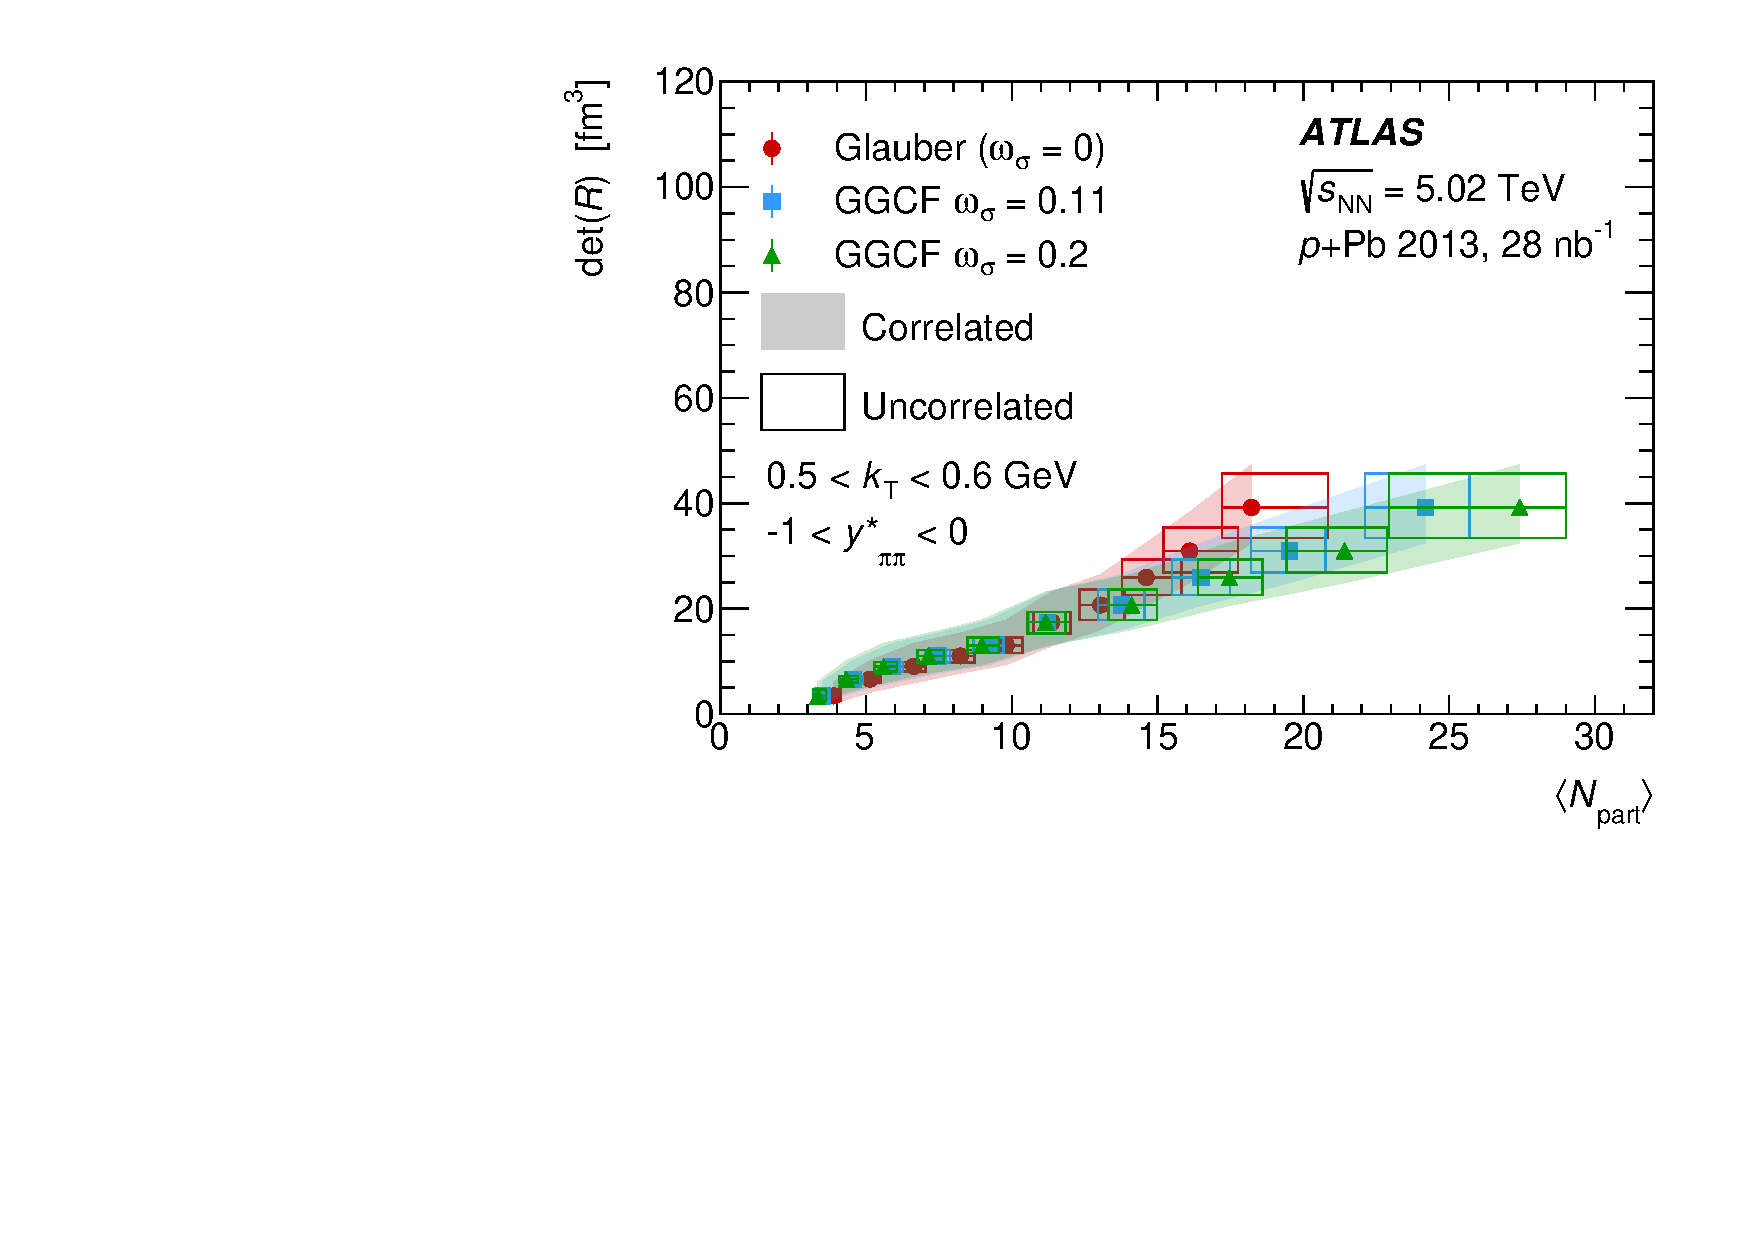
\includegraphics[width=0.49\linewidth]{canqosl_detR_kt4_ggcf.pdf}\\
\caption{The scaling of the volume element, \detR, with \avgNpart calculated with three initial geometry models: standard Glauber as well as Glauber-Gribov (GGCF) for two choices of the color fluctuation parameter, $\omega_\sigma$.
Each of the panels shows a different \kt interval.
The systematic uncertainties from the pion identification and the generator and collision system components of the background description are treated as correlated and shown as error bands.
The systematic uncertainties from charge asymmetry, \Reff, rapidity variation of the jet background, and two-particle reconstruction are treated as uncorrelated and indicated by the height of the boxes.
The horizontal error bars indicate the systematic uncertainties in \avgNpart.}
\label{fig:results_detR_ggcf}
\end{figure}

The determinant of the 3D radius matrix, \detR, is shown in \cref{fig:results_detR_dndeta} as a function of both the average and local density.
While the transverse area scales linearly with  multiplicity at low \kt, the volume scale grows linearly at higher \kt, implying a constant freeze-out volume density for particles with higher momentum.
\cref{fig:results_detR_ggcf} compares the volume scaling with \avgNpart for the standard Glauber model as well as for two choices of the \ac{GGCF} model \cite{Alvioli:2013vk}.
The parameter $\omega_{\sigma}$ controls the size of the fluctuations in the nucleon-nucleon cross section within the \ac{GGCF} model.
With the Glauber model, the scaling of the volume element with \avgNpart has a significant upwards curvature.
Including Glauber-Gribov fluctuations in the \avgNpart calculation results in a more modest curvature in the scaling of \detR.
This result suggests that the fluctuations in the nucleon-nucleon cross section are a crucial component of the initial geometry description in \pPb systems.
The values and systematic uncertainties of \avgNpart in each model are listed in \cref{table:npart}.

\begin{figure}[t]
\centering
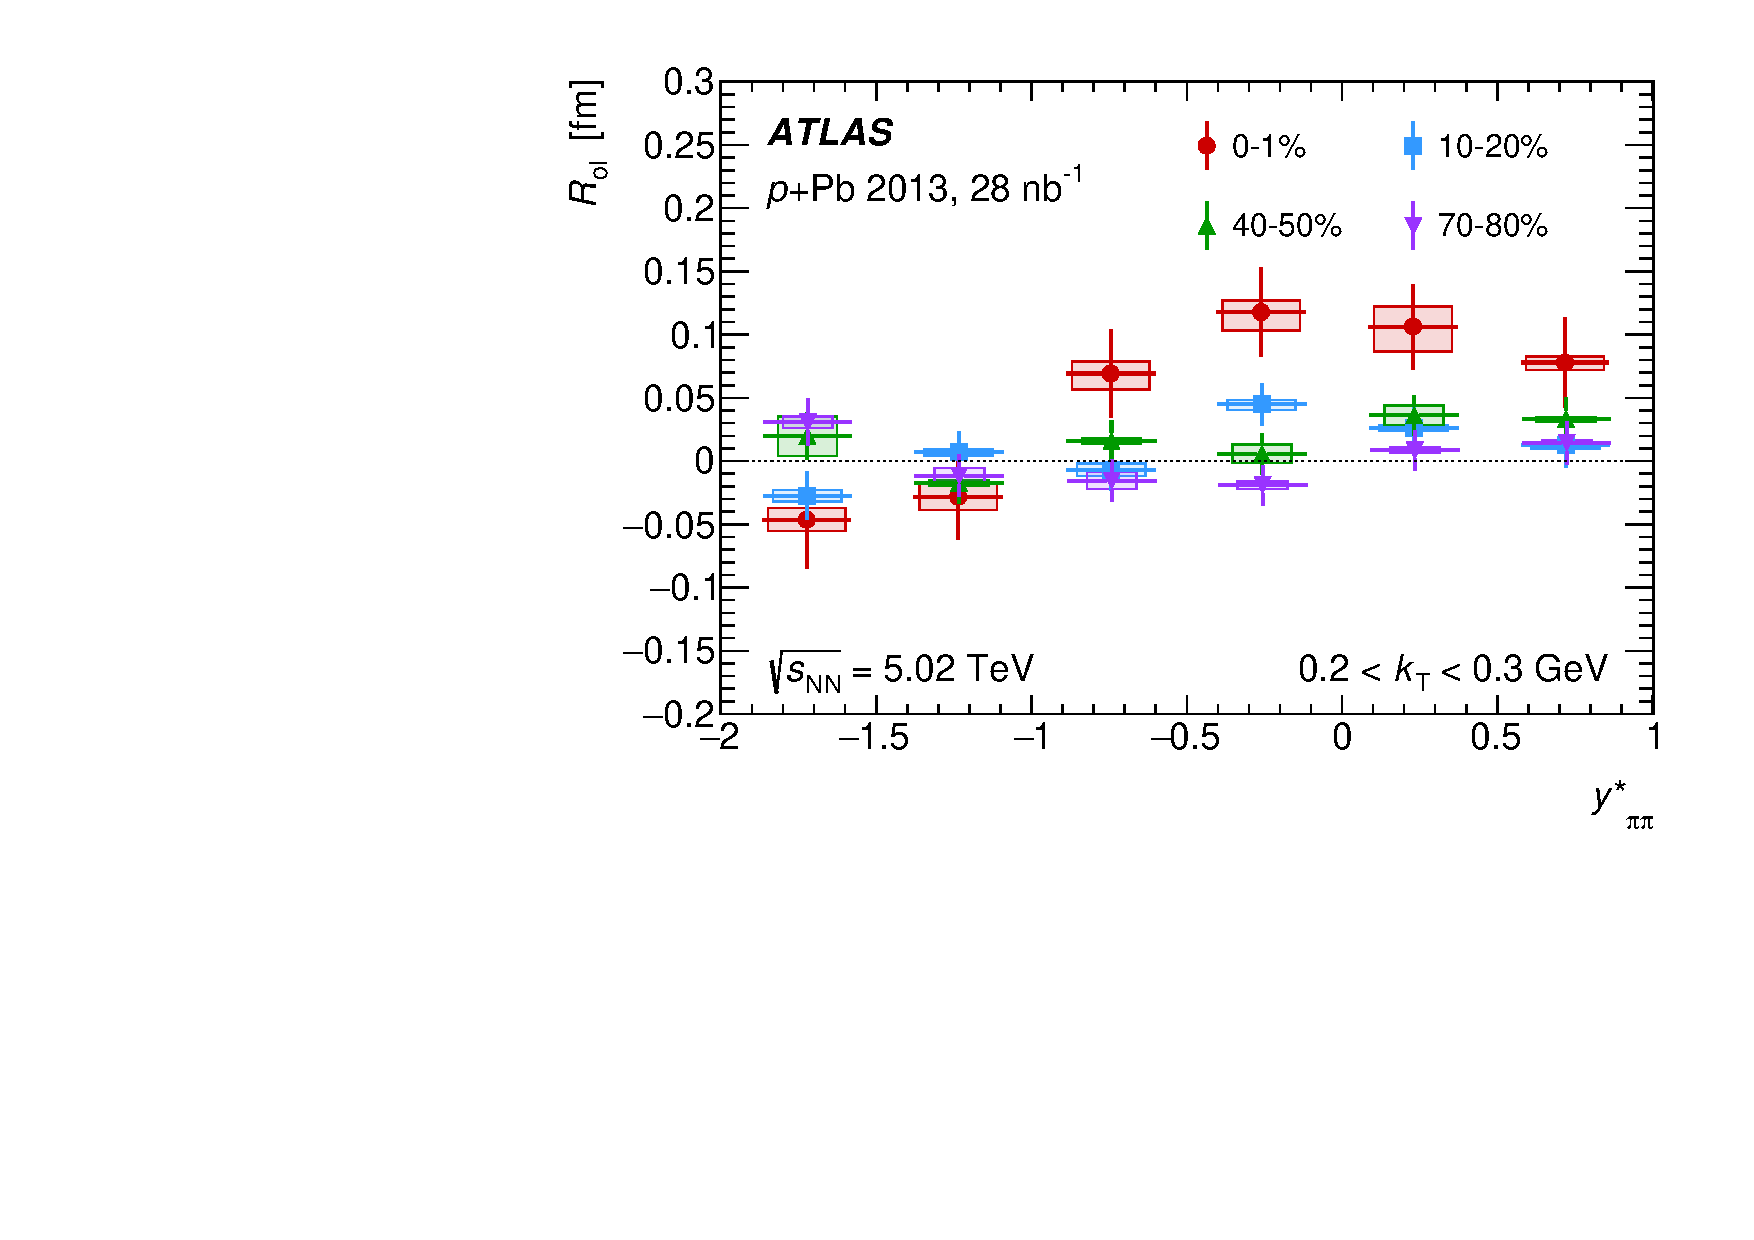
\includegraphics[width=0.49\linewidth]{canqosl_Rol_kt1_vs_kys.pdf}
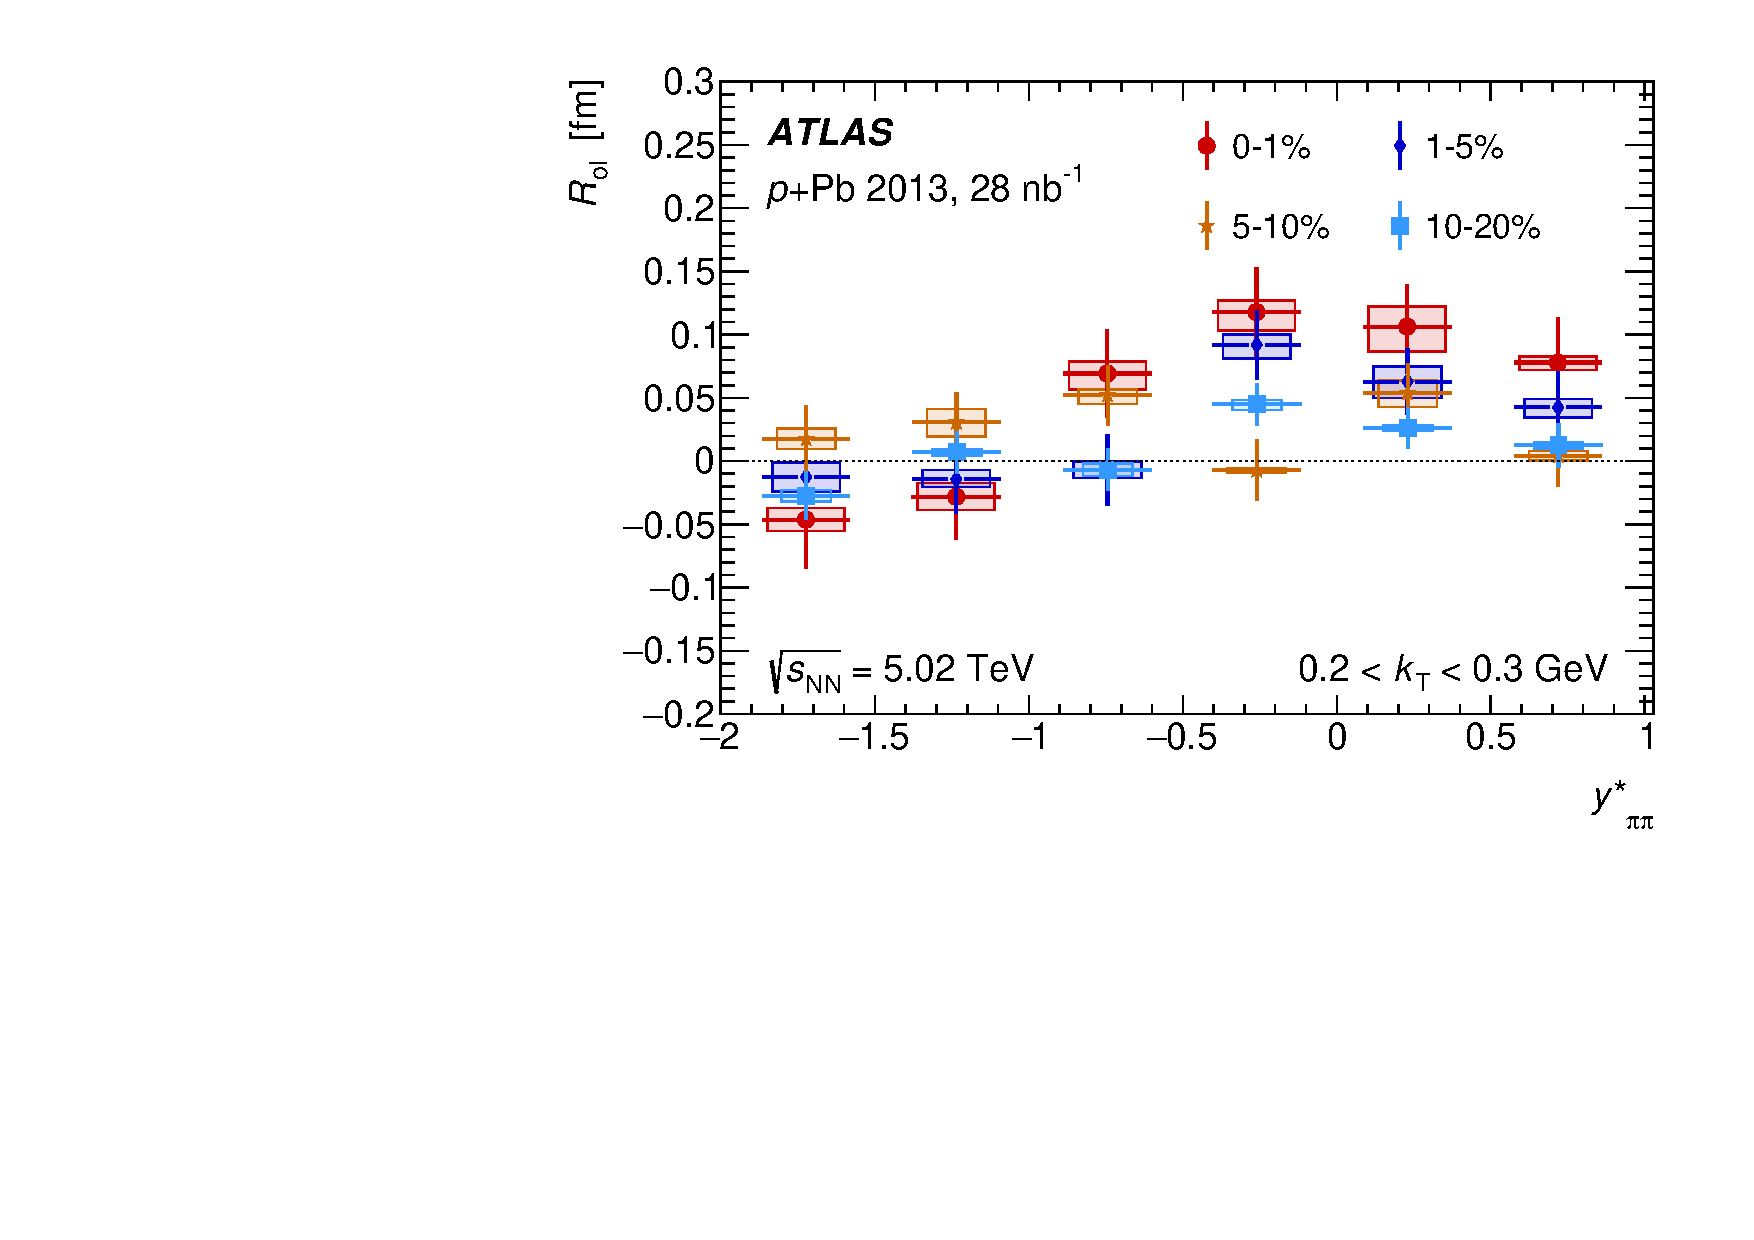
\includegraphics[width=0.49\linewidth]{canqosl_Rol_kt1_vs_kys_altcent.pdf}
\caption{The cross-term, \Rol, as a function of the pair's rapidity, \kys, in a wide range of centrality intervals (left) and in the four most central event classes (right). The vertical size of each box represents the quadrature sum of the systematic uncertainties described in \cref{sec:systematics}, and statistical uncertainties are shown with vertical lines. The horizontal positions of the points are the average \kys in each interval, and the horizontal lines indicate the standard deviation of \kys in the corresponding interval. The widths of the boxes differ only for visual clarity.}
\label{fig:results_Rol_kys}
\end{figure}

\begin{figure}[t]
\centering
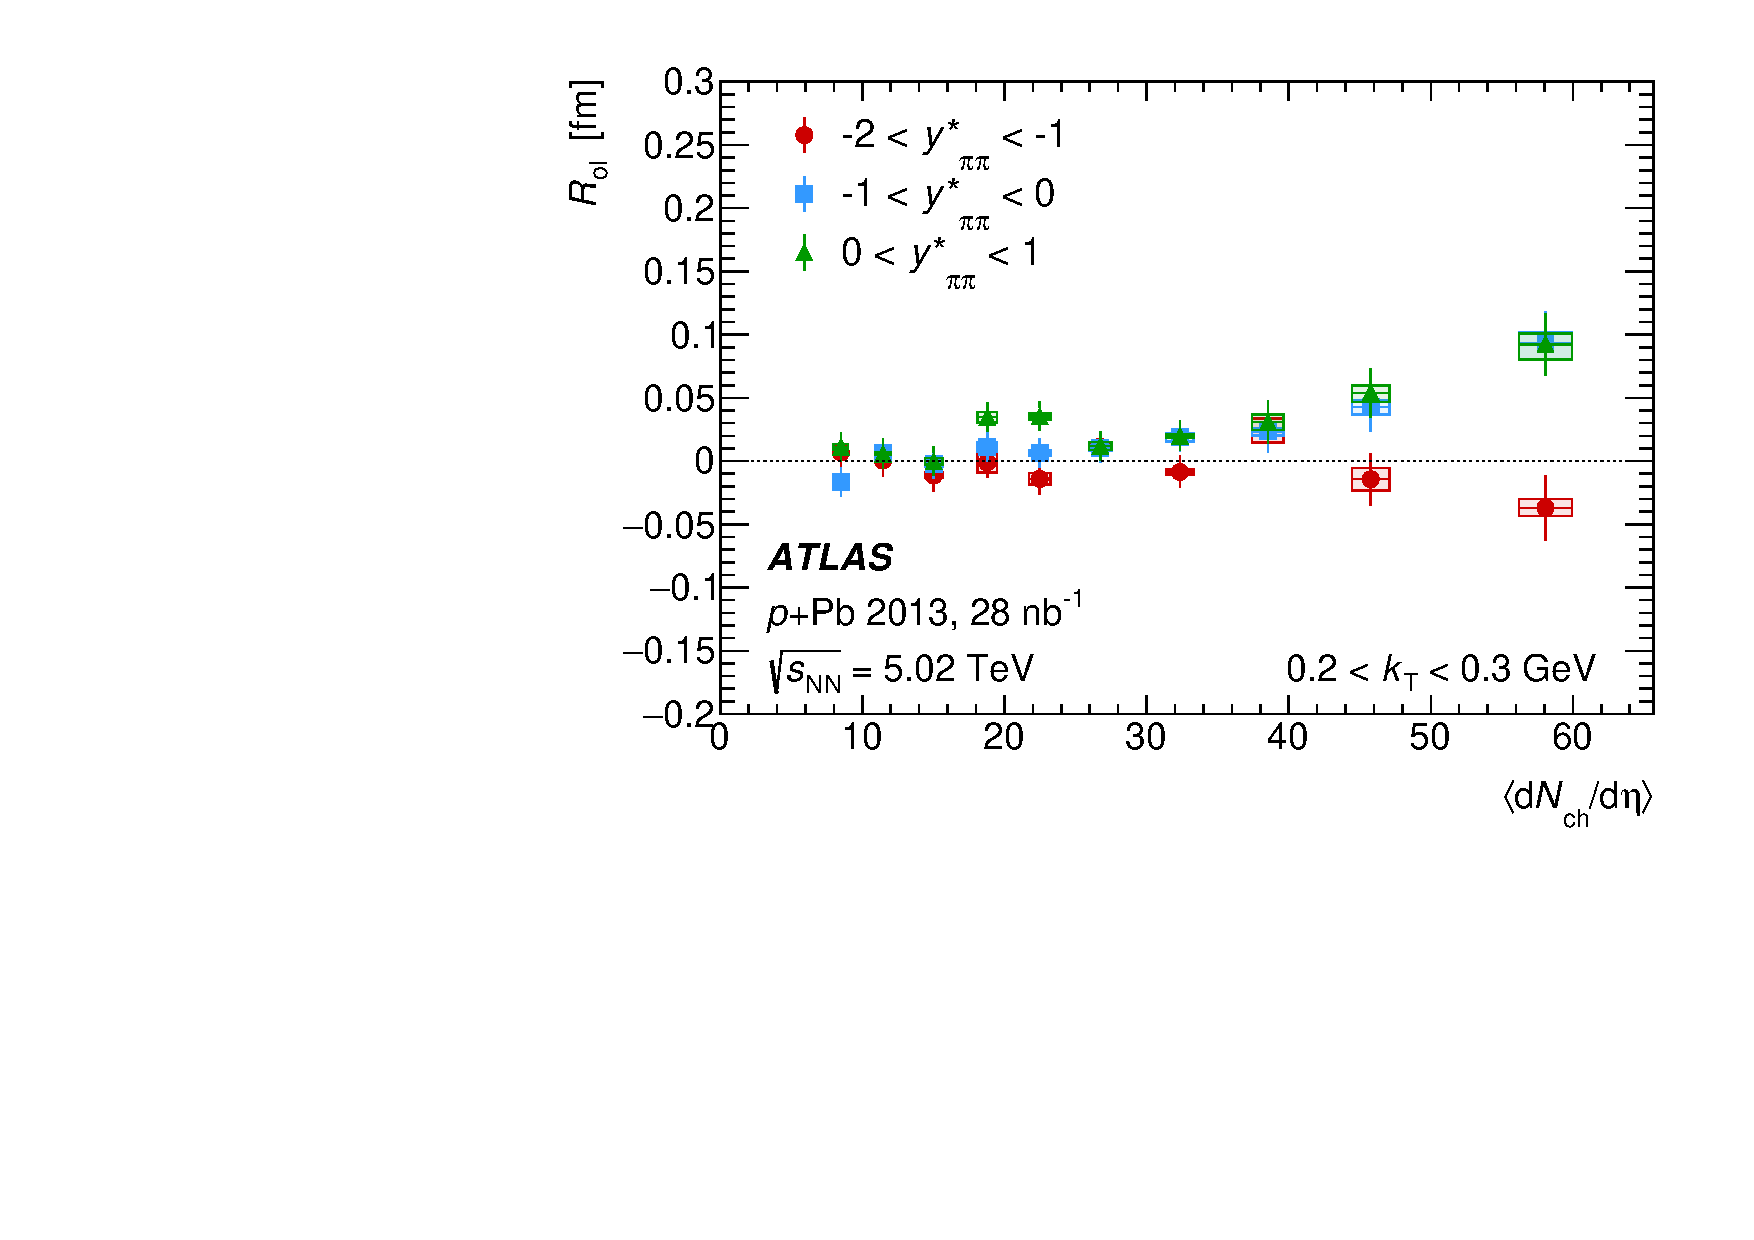
\includegraphics[width=0.49\linewidth]{canqosl_Rol_kt1_kys_vs_avg_mult.pdf}
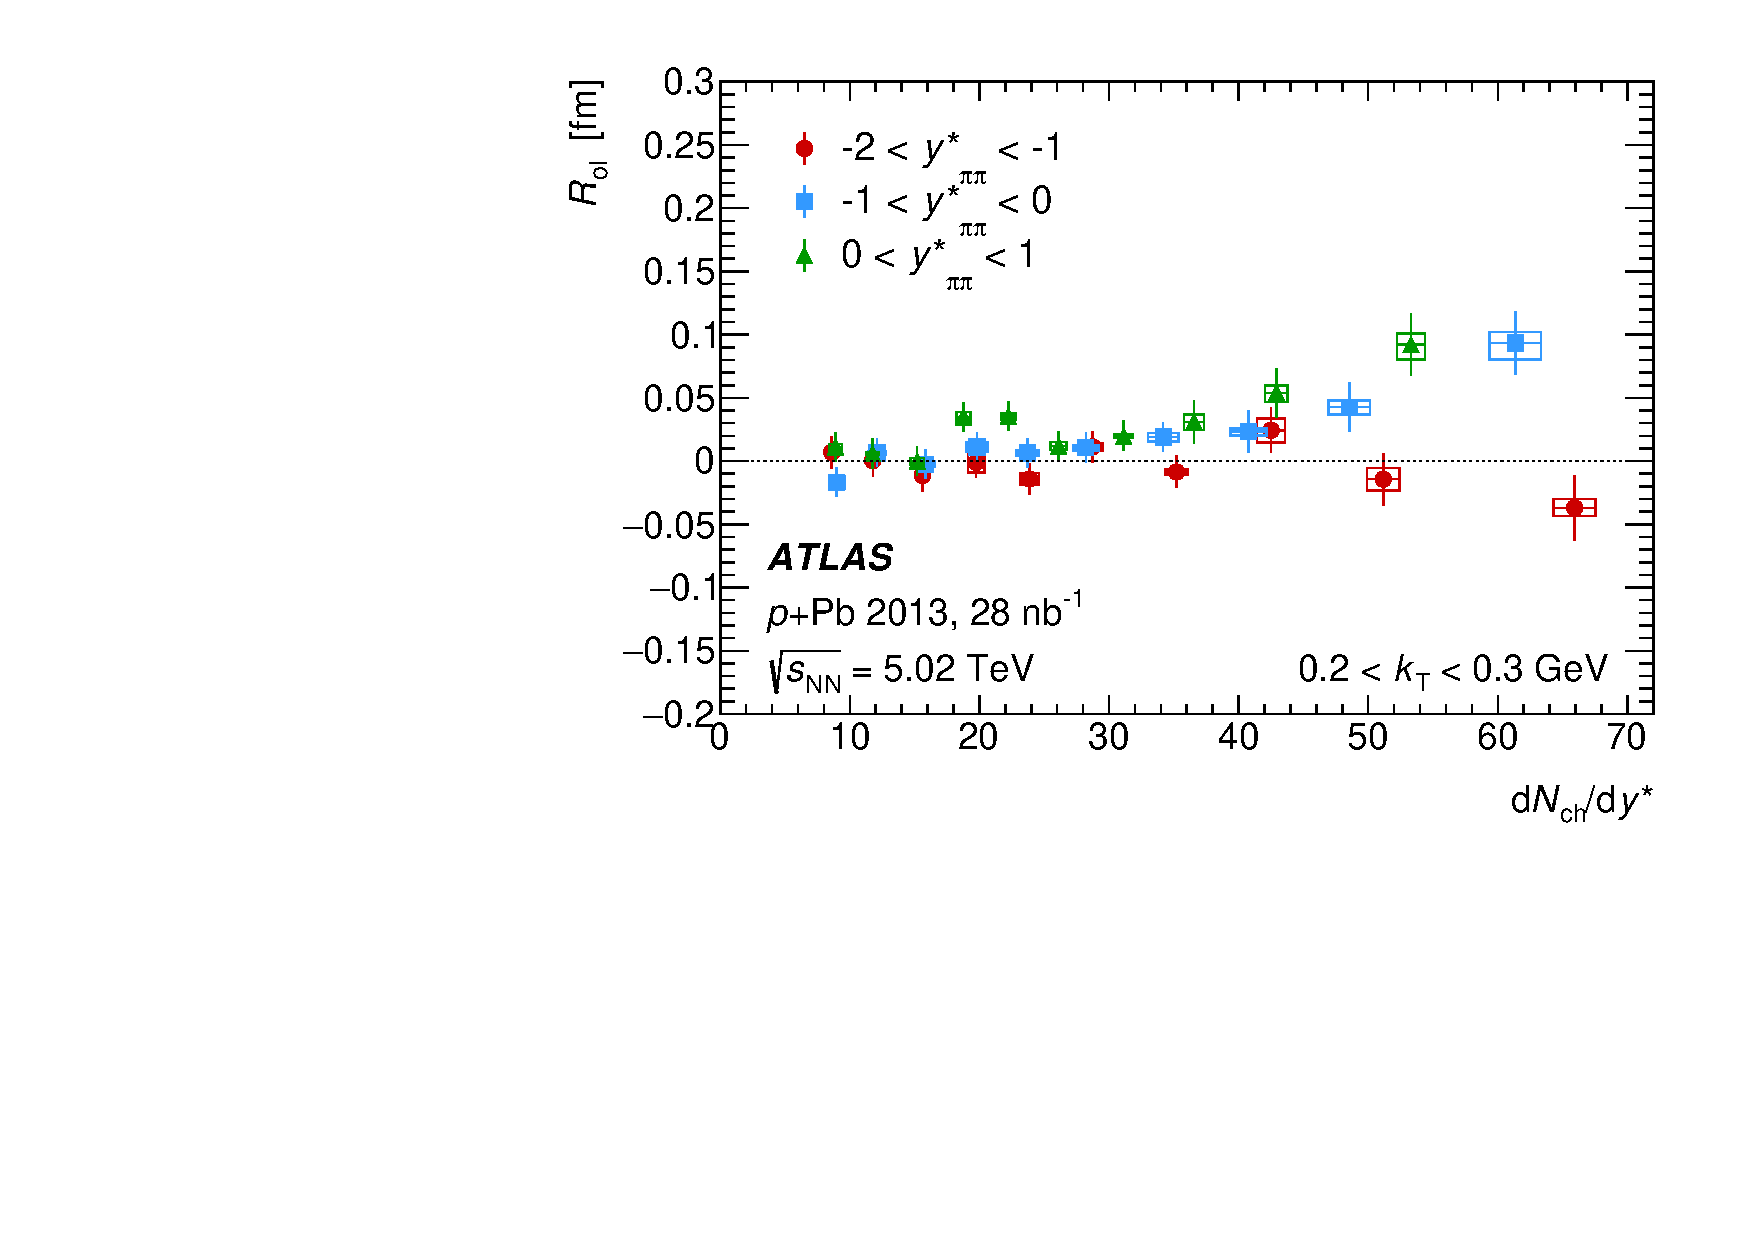
\includegraphics[width=0.49\linewidth]{canqosl_Rol_kt1_vs_mult.pdf}
\caption{The cross-term, \Rol, as a function of average event multiplicity, \avgdNdeta, (left) and the local density, \dNdy (right). The vertical size of each box represents the quadrature sum of the systematic uncertainties described in \cref{sec:systematics}, and statistical uncertainties are shown with vertical lines. The widths of the boxes indicate the systematic uncertainties in the corresponding quantities.}
\label{fig:results_Rol_mult}
\end{figure}

The cross-term, \Rol, which couples to the lifetime of the source \cite{Chapman:1994yv}, is shown in \cref{fig:results_Rol_kys,fig:results_Rol_mult}.
A significant departure from zero is observed in this parameter in central events, but only for rapidities $\kys \gtrsim -1$.
For the 0--1\% centrality interval, in $ 0.2 < \kt < 0.4$ and $-1 < \kys < 1$, \Rol is measured to be nonzero with a significance of 7.1/7.3/5.1 $\sigma$ (statistical/systematic/combined).
The next most central interval, 1--5\%, has a nonzero \Rol with a significance of 5.2/5.8/3.9 $\sigma$ (statistical/systematic/combined).
This suggests that the particle production at middle and forward rapidities is sensitive to the local $z$-asymmetry of the system.

The argument from \cref{subsubsec:coordinate} for why the order of the particles in a pair can be chosen so that \qout is greater than zero relies on the assumption that both particles in the pair are the same species, or at least that they are characterised by the same momentum distributions.
In principle, final-state interactions between different particle species could break this symmetry of the correlation function and lead to a nonzero \Rol term. 
However, the systematic uncertainties shown in \cref{fig:syst_qosl_Rol} demonstrate that \Rol is not sensitive to particle identification, particularly at low \kt.
At larger \kt the systematic effect from \ac{PID} looks larger, but the variations are likely driven by statistical fluctuations.

%% \subsection{Transverse momentum dependence}
%% \subsection{Centrality dependence}
%% \subsection{Pseudorapidity dependence}
\subsection{Comparison with hydrodynamic model}

Interferometry radii have been calculated in recent hydrodynamic simulations of central \pPb collisions \cite{Bozek:2017bwp}.
In general the agreement is quite good with the experimental HBT radii from central collisions with ATLAS.
The theoretical predictions overstate \Rside in comparison to the data, and understate \Rlong at low \kt, but overall capture the \kt-dependence of the radii well, as shown in \cref{fig:results_theory_kt}.
The tilt of the rapidity dependence, shown in \cref{fig:results_theory_kys}, is not as large in the simulations as it is in the data, though the slope of the radii with respect to \kys is in qualitative agreement.
The rapidity dependence of the out-long cross-term, in the fourth panel of \cref{fig:results_theory_kys}, exhibits remarkable agreement between theory and experiment in both magnitude and shape.
These calculations show that hydrodynamics provides an accurate description of ultra-central (0--1\%) \pPb collisions.

\begin{figure}[t]
\centering
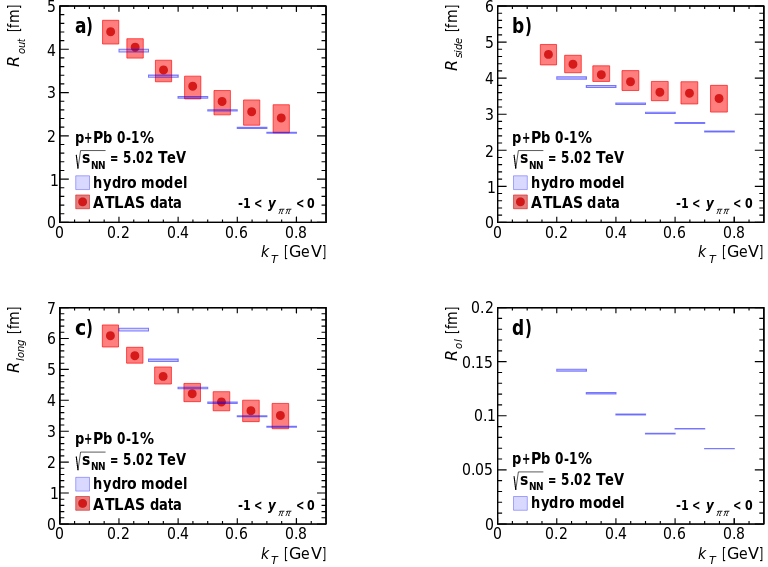
\includegraphics[width=\linewidth]{theory_bozek_kt.png}
\caption{Comparison of ATLAS HBT radii in central \pPb collisions to theoretical hydrodynamic calculations from \Ref{\cite{Bozek:2017bwp}}. The three main HBT radii \Rout, \Rside, and \Rlong as well as the out-long cross-term \Rol are shown as a function of pair transverse momentum \kt.}
\label{fig:results_theory_kt}
\end{figure}

\begin{figure}[t]
\centering
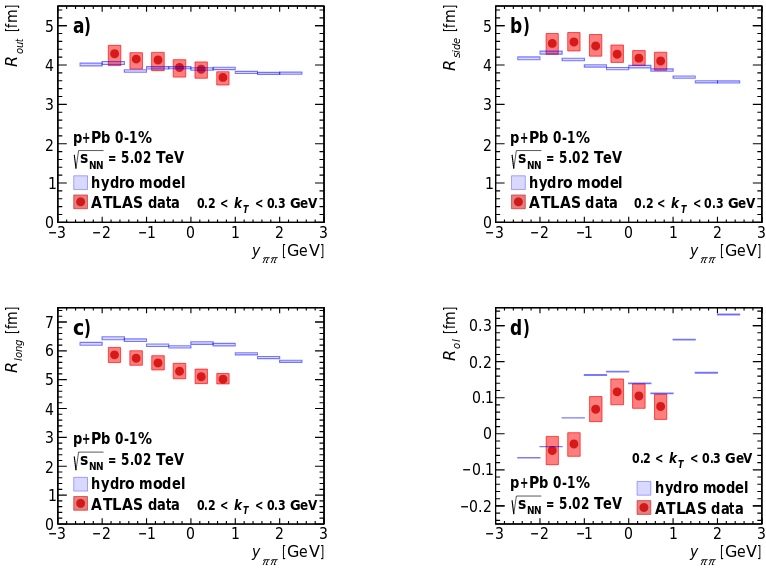
\includegraphics[width=\linewidth]{theory_bozek_kys.png}
\caption{Comparison of ATLAS HBT radii in central \pPb collisions to theoretical hydrodynamic calculations from \Ref{\cite{Bozek:2017bwp}}. The three main HBT radii \Rout, \Rside, and \Rlong as well as the out-long cross-term \Rol are shown as a function of rapidity \kys.}
\label{fig:results_theory_kys}
\end{figure}


\subsection{Azimuthal dependence}

\todo{fill in azimuthal results and discussion, ideally after an iteration on paper draft}
